\documentclass[11pt]{article}

\usepackage[margin=1in]{geometry}
\usepackage{amsmath,amssymb,amsthm,mathtools}
\usepackage{mathrsfs}
\usepackage{booktabs}
\usepackage{array}
\usepackage{graphicx}
\usepackage{placeins}
\usepackage[font=small,labelfont=bf]{caption}
\usepackage{microtype}
\usepackage{natbib}
\usepackage[hidelinks]{hyperref}
\usepackage[nameinlink,noabbrev]{cleveref}

\newtheorem{theorem}{Theorem}[section]
\newtheorem{proposition}[theorem]{Proposition}
\newtheorem{lemma}[theorem]{Lemma}
\newtheorem{corollary}[theorem]{Corollary}
\newtheorem{conjecture}[theorem]{Conjecture}
\theoremstyle{definition}
\newtheorem{definition}[theorem]{Definition}
\theoremstyle{remark}
\newtheorem{remark}[theorem]{Remark}

\newcommand{\R}{\mathbb{R}}
\newcommand{\E}{\mathbb{E}}
\newcommand{\cL}{\mathcal{L}}
\newcommand{\norm}[1]{\left\lVert #1\right\rVert}
\newcommand{\od}{\mathbin{\odot}}
\newcommand{\dd}{\,\mathrm{d}}
\newcommand{\diag}{\operatorname{diag}}
\newcommand{\Law}{\operatorname{Law}}
\newcommand{\HS}{\mathrm{HS}}

\title{{\fontsize{14}{17}\selectfont\bfseries
Compressing Global Dynamics of Deep Nonlinear Feature Learning}}
\author{Amir Joudaki}
\date{September 28, 2026}

\renewcommand{\topfraction}{0.85}
\renewcommand{\bottomfraction}{0.6}
\renewcommand{\textfraction}{0.1}
\renewcommand{\floatpagefraction}{0.8}

\begin{document}
\maketitle

\begin{abstract}
How much can the training dynamics of a deep network be compressed?
Compressing a trained function does not by itself compress its learning:
networks that agree on every input can diverge once training resumes.
We retain depth, effective nonlinearity and feature learning, and replace
each neuron's response history by finitely many evolving Legendre moments
in a clock driven by residual RMS.  The resulting autonomous dynamics
reconstruct the learned interactions while retaining the initialized
matrices exactly.  For fixed depth and training data, canonical Gaussian
initialization, zero initial readout and sufficiently small fixed labels,
we prove exponential fitting at every memory order and approximation
through the entire training trajectory.  Against the dense population
predictor, the whole-input test error is at most
$Cq^{-2}\exp\{K\sqrt{\log(e+q)}\}$ plus a width remainder that vanishes
in probability; the constants are independent of width and time.
Every diverging order $q=o(n)$ therefore reaches the same population
learning process with $O(Lmnq)$ evolving history coordinates instead of
$O(Ln^2)$ learned weights.  Broader-label finite-time guarantees and an
exact hidden-learning-rate rescaling describe extensions of the central
regime.  Circle, sphere and MNIST experiments show that small memory
orders reproduce dense fitted predictions on unseen inputs, while the
tested frozen-kernel and rank-matched factor baselines can select
substantially different functions.  The result isolates a compressible
part of deep learning: the response memory that carries its evolving
interactions.
\end{abstract}

\section{Introduction}

\paragraph{A missing model of learning.}
The Turing machine is the canonical model of computation.  It is idealized---it
has no fixed bound on memory---and it is simple enough to reason about,
while physical computers, from the von Neumann architecture onward, are
understood as its finite-resource implementations.  One might view neural networks
as playing the role in learning that physical computers play in computation;
what this analogy still lacks is a counterpart to the Turing machine---a
canonical idealized model of learning.  Deep neural networks trained by gradient
descent are the obvious candidates for implementations of such a model, but the
object they would implement is not yet known.  The obstacle is that their
training dynamics are enormously complex and have no simple representation.

\paragraph{The limit, and why to compress it.}
A natural place to look for the idealized object is the limit of infinite width.
Under feature-learning scalings of the type used in tensor-program and mean-field
theory \citep{yang2021tensor,nguyen2023rigorous}, width-dependent learning rates
preserve order-one feature evolution, and suitable population observables obey
deterministic limiting laws.  The limit is the network with no resource
constraint, as the Turing machine is the computer with none; a finite network
would then be this limit plus a quantified deviation from it, as in a central
limit theorem.  Going to infinite width to simplify seems paradoxical, since the
dynamical system grows with width.  Statistical physics resolves the paradox in
other settings: a gas of $10^{23}$ molecules is simpler to describe than a gas
of ten, because its macroscopic behaviour is captured by a few collective
variables.  Training presents two sources of complexity: the number of neurons,
and the response history introduced when evolving weights are eliminated from
the description.  The weights themselves are a Markovian state; response-based
limits express their learned interactions through the past.  Mean-field and
tensor-program limits address width.  Whether the response history can also be
\emph{compressed} is our question.  We do not seek compression for its own
sake: a compressed description must retain what drives learning and may discard
the rest, so the state that survives is a candidate for the variables that
govern learning, and a compressed system that reproduces training would be a
step toward the idealized model.

\paragraph{What the model must keep.}
Several influential simplifications isolate different aspects of training.
Deep linear networks admit exact solutions but remove the
nonlinearity \citep{saxe2014exact}; one-hidden-layer mean-field models remove
multilayer hidden interactions \citep{chizat2018global,mei2018meanfield,sirignano2019lln}; and
the neural tangent kernel keeps depth and nonlinearity but freezes the features
\citep{jacot2018ntk,lee2019wide,chizat2019lazy}.  Each is simple precisely
because of what it gives up.  Our target keeps all three: \emph{depth} (more than one
hidden layer), \emph{nonlinearity} that stays effective during training and in
the limit, and \emph{feature learning} (hidden representations move at leading
order).  It must also reproduce the whole trajectory, not a snapshot: two
networks that compute the same function on every input can have different
Jacobians and backward responses, and once training resumes the discrepancy
accumulates.  Together with a specified population limit, this contract fixes
the object we seek to understand.

\paragraph{The gap, and one axis for every description.}
Width compression leaves a further resource question.  Tensor Programs
carry variables indexed by every earlier training step \citep{yang2021tensor},
and feature-learning dynamical mean-field theory (DMFT) evolves two-time kernels
whose memory grows quadratically with the number of time points
\citep{bordelon2022dmft}.  These descriptions encode learned interactions
through temporal responses rather than explicit learned matrices, a
substantial reduction in width dependence, but their state grows with the
number of retained time points.  We ask whether evolving learned interactions
can instead be carried by a fixed number of neuron-level coordinates, with a
bound on the error of the complete training trajectory.  The question suggests
one axis on which every description of training can be placed: fix a horizon
and an accuracy, and ask how much \emph{evolving} state a description needs to
reproduce the trajectory to that accuracy, and whether that state grows with
the number of elapsed steps.  Descriptions that freeze the features, drop depth
or drop the nonlinearity target a different training regime, and enlarging
their state alone supplies no general approximation guarantee for ours.  Those
that keep the contract each pay for the limit in a different currency: the
dense network in neurons, Tensor Programs and DMFT in stored history, the Neural
Tangent Hierarchy in tensors indexed by tuples of training samples.  Response
memory pays in an approximation order: no coordinates are added merely
because more steps elapse.  Under the small-label conditions proved below,
one order controls the entire physical-time interval; more generally the
required order can depend on the horizon and the task.  \Cref{def:global} makes
the axis precise, \Cref{tab:axis} (\Cref{sec:related}) places the descriptions
on it once the results are in hand, and \Cref{app:size} works out, under stated
hypotheses, what each would cost at a prescribed accuracy.

\paragraph{Key contribution.}
The learned matrix is a paired memory of forward and backward responses.
We compress that memory into an autonomous dynamics and control its feedback
on the signals it records.  Our central theorem makes this statement uniform
over the whole learning process: in a small-label Gaussian regime, every
memory order fits exponentially, and order $q$ tracks the dense population
predictor with error $q^{-2+o(1)}$ plus a vanishing width remainder
(\Cref{thm:alltime}).  The regime permits any fixed depth and a broad class
of nonlinear activations; labels are small but fixed as width grows, and
hidden learning retains its canonical scaling.  As a consequence, any
diverging order $q=o(n)$ converges to the same limiting predictor while
using a vanishing fraction of the dense model's evolving state
(\Cref{cor:compression}).  This is compression of an entire learning
trajectory, not a factorization of its endpoint.  Small orders reproduce
the fitted function in experiments where frozen kernels and rank-matched
trained factors do not (\Cref{sec:experiments}).

\section{Setting}
\label{sec:setting}

Fix $m$ training pairs $(x_a,y_a)$ with $x_a\in\R^d$, width $n$ and $L\ge2$
hidden layers:
\begin{align}
 z_a^{(1)}&=W^{(1)}x_a/\sqrt d,& h_a^{(1)}&=\phi(z_a^{(1)}),\nonumber\\
 z_a^{(\ell)}&=W^{(\ell)}h_a^{(\ell-1)},&
 h_a^{(\ell)}&=\phi(z_a^{(\ell)}),\quad 2\le\ell\le L,\\
 f_a&=\frac{w^\top h_a^{(L)}}{n},& r_a&=f_a-y_a,\qquad
 \rho=\Bigl(\frac1m\sum_a r_a^2\Bigr)^{1/2}.\nonumber
\end{align}
The activation $\phi$ may differ between layers; the loss is $\cL=\rho^2$.  The
backward responses, which exclude the residual, are
$\delta_a^{(L)}=w\od\phi'(z_a^{(L)})$ and
$\delta_a^{(\ell)}=\phi'(z_a^{(\ell)})\od(W^{(\ell+1)})^\top\delta_a^{(\ell+1)}$.
With block mobilities $(n,1,\ldots,1,n)$, gradient flow reads
\begin{equation}
 \dot W^{(1)}=-\frac2m\sum_a r_a\delta_a^{(1)}\frac{x_a^\top}{\sqrt d},\quad
 \dot W^{(\ell)}=-\frac{2}{nm}\sum_a r_a\delta_a^{(\ell)}
 (h_a^{(\ell-1)})^\top\ (2\le\ell\le L),\quad
 \dot w=-\frac2m\sum_a r_a h_a^{(L)}.\label{eq:dense-flow}
\end{equation}
We write $\theta=(W^{(1)},\ldots,W^{(L)},w)$ for all parameters and
$\dot\theta=F(\theta)$ for \eqref{eq:dense-flow}.  Hidden entries are initialized
as $\mathcal N(0,1/n)$, first-layer entries as $\mathcal N(0,1)$, and the stored
readout is specified by the result being applied; the central theorem uses
$w(0)=0$ exactly.

For comparisons across widths we use the normalized parameter distance
\begin{equation}
 d_n(\widehat\theta,\theta)
 =\frac{\|\widehat W^{(1)}-W^{(1)}\|_F}{\sqrt n}
 +\sum_{\ell=2}^L\|\widehat W^{(\ell)}-W^{(\ell)}\|_F
 +\frac{\|\widehat w-w\|_2}{\sqrt n}.
 \label{eq:normalized-distance}
\end{equation}
These scalings agree with the block mobilities and with order-one
forward predictions.

\paragraph{Population flow.}
As $n\to\infty$, the neurons of layer $\ell$ become a probability space
$\Omega_\ell$ with expectation $\E_\ell$: hidden coordinates $z^{(\ell)},h^{(\ell)}$
become random variables in $L^2(\Omega_\ell)$, the first-layer weights a random
row $W^{(1)}\in L^2(\Omega_1;\R^d)$, the readout $w\in L^2(\Omega_L)$, and each
hidden matrix a bounded operator $W^{(\ell)}:L^2(\Omega_{\ell-1})\to L^2(\Omega_\ell)$
used together with its true adjoint.  The same equations \eqref{eq:dense-flow}
hold with $\frac1n\sum_i$ replaced by $\E_\ell$ and outer products
$\delta\,h^\top/n$ by the rank-one operators $g\mapsto\delta\,\E[h\,g]$.  Such
limits are established in several scopes---for fixed depth on a short horizon,
and globally in special models---with finite-width gradient flow converging to
them on compact horizons; a global theorem for general data and depth is open.
In the small-label regime of \Cref{thm:alltime}, the Gaussian construction
and the finite-activity estimate identify the dense population predictor
for all physical time.  The proof is included in \Cref{app:proof-alltime}.

\paragraph{What counts as compression.}
An exact compression reproduces the reference trajectory; an approximate one
reproduces it up to a controllable error.  A compression may also match the
current state and velocity while its small errors compound until the
trajectories separate; we ask for the stronger, global notion.

\begin{definition}[Global approximation on compact horizons]
\label{def:global}
Autonomous systems indexed by an order $q$, with trajectories $\theta_q$,
\emph{globally approximate} a reference flow $\theta$ if for every $T<\infty$
\[
  \sup_{0\le t\le T}\norm{\theta_q(t)-\theta(t)}\longrightarrow0
  \qquad(q\to\infty).
\]
The rate in $q$ quantifies the trade-off between the size of the compressed
state and its accuracy.  We call the approximation \emph{all-time} when the
same conclusion holds with the supremum over $t\ge0$.  Our central result
establishes this stronger notion, with an additional vanishing width
remainder when the target is the population flow.
\end{definition}
The size in question is the \emph{moving state} of a description: the numbers
it updates while computing training, excluding fixed sources such as the
initialization or a frozen kernel.

\section{Closing the training dynamics: exact and approximate}
\label{sec:memory}

\subsection{Exact closure: operators and an obstruction}
\label{sec:notions}

A closed description of training evolves a state of one of three kinds: finitely
many \emph{scalars}, independent of width and training time; finitely many
\emph{populations} (functions, random variables or laws on fixed spaces, such as
the law of a neuron's weights), whose particle implementation stores one value
per particle and field; or \emph{operators} between population spaces, the
limits of matrices, which record how each row relates to each column, a
coupling that one-neuron marginal statistics discard.  A finite number of named
fields or operators need not contain finitely many scalars, so every claim below
names both the type and the size of the retained state.

Before allowing errors we ask what exact capture of the population flow can look
like.  A natural candidate without growing history is an operator ODE:
\eqref{eq:dense-flow} read with the hidden matrices $W^{(\ell)}$ as operators.
In a deep linear benchmark---one input, three linear hidden layers, order-one
initialization---this can be proved completely: the learned part of the whole
network becomes a single trace-class operator that evolves by an explicit
autonomous cubic equation driven by the residual, and finite gradient flow and
gradient descent converge to it on every compact horizon in the stated limits
(\Cref{app:exact}).  But one named operator can contain infinitely many degrees
of freedom, so an operator equation alone supplies no finite state--accuracy
trade-off; such a trade-off requires a further approximation of the operator.
At the other extreme, in the same linear benchmark no encoder formed from a
fixed finite list of tensor contractions of the weights with width-independent
bounded degree admits a polynomial autonomous scalar ODE and polynomial readout
that reproduce the output dynamics on an open set of states at all large widths
(\Cref{app:exact}).  The reason is that repeated differentiation of the output
forces ever larger connected contractions: the $(2j-1)$st derivative contains
$\frac1n\,(W^{(1)})^\top\bigl((W^{(2)})^\top(W^{(3)})^\top W^{(3)}W^{(2)}\bigr)^{j}W^{(1)}$,
of degree $4j+2$, which no bounded-degree alphabet can express.  The result is
restricted to this encoder and readout class; it identifies a concrete obstacle
already present with linear features, not a no-go theorem for all finite scalar
descriptions.  Between the two, whether the exact operator can be compressed
into finitely many populations is open: rank-one gradient updates do not by
themselves imply a fixed rank bound on their time integral.  The main result
takes a constructive route: accepting controlled error gives an explicit
autonomous system with a quantitative state--accuracy trade-off.

\subsection{Approximate closure: the idea}

Integrating \eqref{eq:dense-flow}, every hidden matrix is
\begin{equation}
 W^{(\ell)}(t)=W_0^{(\ell)}-\frac{2}{nm}\sum_a
 \int_0^t r_a(s)\,\delta_a^{(\ell)}(s)\,
 (h_a^{(\ell-1)}(s))^\top\dd s .                        \label{eq:exact-history}
\end{equation}
The learned part is an integral of backward against forward responses.  Two
direct representations are the dense matrix and the accumulated response
history.  A familiar analogy is a moving ball: under a known force law, its
current position and velocity can determine the future without storing its past
positions.  Here we seek history coordinates that retain enough information
for the network's own law of motion.  Regular response histories suggest that
a few coefficients can summarize the interaction integral.  Two things must
hold: the summary must be
\emph{closed}, so that it evolves autonomously, and \emph{accurate} over the
whole of training, which alternates between bursts of learning and plateaus.

\subsection{Closure: shifted Legendre moments}

Let $p_k$ be the shifted Legendre polynomials on $[0,1]$, normalized by
$p_k(1)=1$ and $\int_0^1p_jp_k=\mathbf 1_{j=k}/(2k+1)$.  Their derivatives reduce
to lower modes,
\begin{equation}
 x\,p_k'(x)=k\,p_k(x)+\sum_{j<k}(2j+1)\,p_j(x),        \label{eq:triangular}
\end{equation}
and this is what makes the moment system close exactly.  The identity underlies
online polynomial memory in HiPPO \citep{gu2020hippo}; the new element is that
the memorized signals are the network's own forward and backward responses,
coupled back through the reconstructed network.
The first moments of a history are its mean, its linear trend (the first
polynomial rises from $-1$ at the start to $1$ now) and its quadratic shape;
each added moment corrects what the previous ones miss (\Cref{fig:moments}, \Cref{app:supp-figs}).

\subsection{Accuracy: a clock that follows learning}

Concentrated variation can require many polynomial modes in physical time.
We therefore measure history in a clock
$\tau$ that runs at the speed of learning,
\begin{equation}
 \dot\tau=\rho,\qquad \tau(0)=1:                        \label{eq:old-clock}
\end{equation}
fast when the residual is large and slow as it approaches zero.  This speed is
the square root of loss, not its time derivative; it need not stop at a
positive-loss stationary point.  The unit prefix
$[0,1]$ carries the initial forward responses and no backward response.  For
each hidden link $\ell\ge2$ and sample $a$ we store the first $q$ Legendre
moments, in the clock coordinate, of the forward response $h_a^{(\ell-1)}$ and
of the residual-weighted backward response $r_a\delta_a^{(\ell)}/\rho$:
\[
 \bar h^{(\ell-1)}_{a,k}=\int_0^{\tau} h_a^{(\ell-1)}\,p_k(\xi/\tau)\dd\xi,\qquad
 \bar\delta^{(\ell)}_{a,k}=\int_0^{\tau}\frac{r_a\delta_a^{(\ell)}}{\rho}\,
 p_k(\xi/\tau)\dd\xi,\qquad 0\le k<q,
\]
where $\xi$ is the clock value at which each response was recorded.  By
\eqref{eq:triangular} these moments obey the closed system
\begin{align}
 \dot{\bar h}^{(\ell-1)}_{a,k}&=\rho\,h_a^{(\ell-1)}-\frac{\rho}{\tau}
 \Bigl[k\,\bar h^{(\ell-1)}_{a,k}+\sum_{j<k}(2j+1)\,\bar h^{(\ell-1)}_{a,j}\Bigr],\nonumber\\
 \dot{\bar\delta}^{(\ell)}_{a,k}&=r_a\delta_a^{(\ell)}-\frac{\rho}{\tau}
 \Bigl[k\,\bar\delta^{(\ell)}_{a,k}+\sum_{j<k}(2j+1)\,\bar\delta^{(\ell)}_{a,j}\Bigr],
 \label{eq:old-ode}
\end{align}
with $\bar h^{(\ell-1)}_{a,0}(0)=h_a^{(\ell-1)}(0)$ and all other moments zero, and
the hidden matrices are reconstructed as
\begin{equation}
 \widehat W^{(\ell)}=W_0^{(\ell)}-\frac{2}{nm\tau}
 \sum_{a=1}^m\sum_{k=0}^{q-1}(2k+1)\,
 \bar\delta^{(\ell)}_{a,k}\,(\bar h^{(\ell-1)}_{a,k})^\top .   \label{eq:old-recon}
\end{equation}
All responses in \eqref{eq:old-ode} are evaluated in the current
\emph{reconstructed} network, and the first layer and readout follow
\eqref{eq:dense-flow}.  The system is autonomous and never divides by $\rho$.
Equivalently, with $\Pi_q$ the $L^2(0,\tau)$ projection onto polynomials of
degree below $q$,
\begin{equation}
 \widehat W^{(\ell)}=W_0^{(\ell)}-\frac{2}{nm}\sum_a
 \int_0^\tau\Bigl(\Pi_q\frac{r_a\delta_a^{(\ell)}}{\rho}\Bigr)
 \bigl(\Pi_q h_a^{(\ell-1)}\bigr)^\top\dd\xi,               \label{eq:projection-form}
\end{equation}
and since cross terms vanish by orthogonality, the error in each matrix update is
a \emph{product} of a forward and a backward projection error.
\Cref{fig:mechanism}(b) (\Cref{app:supp-figs}) illustrates this cancellation and distinguishes it from
the separate stability argument that controls feedback.

\paragraph{The joint feature-learning clock.}
The learning-speed clock makes forward histories smooth but not every backward
history.  A second clock advances with the residual \emph{plus} the speed of all
forward and backward responses,
\begin{equation}
 \dot\tau=\rho+\Bigl\|\tfrac{d}{dt}\bigl(h_a^{(\ell-1)},\,r_a\delta_a^{(\ell)}/\rho\bigr)_{\ell,a}\Bigr\|_2,
 \qquad\tau(0)=1,                                         \label{eq:new-clock}
\end{equation}
so that the whole response path moves at unit speed at most in the clock
coordinate.  History is placed by this clock but still weighted by the residual
mass $\rho\dd t$, so the Legendre modes are no longer orthogonal and one shared
$q\times q$ Gram matrix is tracked alongside the moments; the reconstruction uses
its inverse, the defect keeps the product form, and the clock speed can be
evaluated explicitly by one directional forward and backward pass
(\Cref{app:proof-new}).
The coordinate change is illustrated in \Cref{fig:clock} (\Cref{app:proof-new}).

\subsection{A uniform approximation of the whole learning process}
\label{sec:alltime}

The central result concerns the learning-speed closure
\eqref{eq:old-ode}--\eqref{eq:old-recon}, with its own residual and responses.
Its accuracy is measured against the function selected by dense training,
including on inputs never used for training.  For a test-input probability
law $\mu$, write
\begin{equation}
 \mathcal E_\mu(g,f)=
 \left(\int\sup_{t\ge0}|g(t,x)-f(t,x)|^2\dd\mu(x)\right)^{1/2}.
 \label{eq:test-metric}
\end{equation}
The supremum is inside the integral: the estimate controls the entire
trajectory at every test input, rather than only a selected stopping time.

\begin{theorem}[All-time response-memory approximation]
\label{thm:alltime}
Fix the depth $L\ge2$, input dimension $d$, and $m$ training inputs.  In each
layer let $\phi_\ell\in C^1(\R)$ have a globally bounded derivative and a
globally Lipschitz derivative.  Use the independent Gaussian initialization
of \Cref{sec:setting}, with $w(0)=0$, and the same initialization for dense
and compressed training.  Assume the limiting initial readout-feature Gram
has a positive gap:
\begin{equation}
 \Gamma_{w,\infty}(0)
 :=\lim_{n\to\infty}\frac{H^{(L)}(0)^\top H^{(L)}(0)}{mn}
 \succeq2\lambda I_m,\qquad \lambda>0,
 \label{eq:initial-gap}
\end{equation}
where the columns of $H^{(L)}$ are the training features.
There is $Y_*>0$, independent of width and order, such that for fixed labels
with $Y=(m^{-1}\sum_a y_a^2)^{1/2}\le Y_*$ the following hold.

There are constants $C,K,\kappa>0$, independent of $n,q,t$, and common
initialization events of probability tending to one, on which the dense
flow and every closure order $q\ge1$ exist for all time and satisfy
\begin{equation}
 \rho_n(t),\ \widehat\rho_{n,q}(t)\le Y e^{-\kappa t}.
 \label{eq:alltime-fit}
\end{equation}
Their parameters converge as $t\to\infty$.  Simultaneously for every order,
\begin{equation}
 \sup_{t\ge0}d_n(\widehat\theta_{n,q}(t),\theta_n(t))
 \le C\omega(q)+b_n,\qquad
 \omega(q)=\frac{\exp\{K\sqrt{\log(e+q)}\}}{q^2},
 \quad b_n\xrightarrow{\Pr}0,
 \label{eq:alltime-parameters}
\end{equation}
where $b_n$ depends only on the dense reference, not on $q$.

The dense predictors converge to a deterministic population predictor
$f_\infty$.  For every fixed $\mu$ with
$\int\|x\|^2\dd\mu(x)<\infty$, there is an order-independent remainder
$b_{n,\mu}\xrightarrow{\Pr}0$ such that, on the same events,
\begin{equation}
 \mathcal E_\mu(\widehat f_{n,q},f_\infty)
 \le C_\mu\omega(q)+b_{n,\mu}.
 \label{eq:alltime-predictions}
\end{equation}
For every fixed bounded input set $\mathcal X$, the analogous bound holds
for $\sup_{t\ge0,x\in\mathcal X}|\widehat f_{n,q}(t,x)-f_\infty(t,x)|$.
Constants may depend on depth, data, activation bounds and the initial Gram
gap.  The label threshold is fixed as $n,q\to\infty$.
\end{theorem}

Thus the order error is $q^{-2+o(1)}$: every fixed exponent below two is
available.  The width remainder is a convergence statement, without an
asserted numerical rate in $n$.  For any square-integrable target function,
the difference between the closure's and the dense population's test RMSE
is at most \eqref{eq:alltime-predictions}, uniformly in time, by the reverse
triangle inequality.  In particular, a circle or sphere is a whole test
domain covered by the theorem; a mesh is needed only to display its function.

The activation class includes tanh, softplus, GELU, SiLU and softsign; its
values need not be bounded.  The Gram condition is an initialization
condition.  One sufficient input criterion is nonzero, pairwise
nonproportional inputs, with a nonpolynomial first activation and nonconstant
subsequent activations in the stated class.  The proof of this criterion and
the theorem are in \Cref{app:proof-alltime}.

\paragraph{Why the bound survives feedback and infinite time.}
Small labels first give a short total interval of learning activity.  This
keeps the initial feature-Gram gap open.  The closure's exact velocity defect
is the product of its forward and backward endpoint projection errors;
their opposite powers of $q$ cancel in a coarse bound relative to the
residual.  This proves exponential fitting for \emph{every} order before
using any approximation-to-dense argument.  The sharper tracking estimate
then uses the projection-energy identity to integrate the defect: its two
history errors multiply.  Gaussian tail control is needed only for the dense
reference's backward carriers.  Cutting those carriers in the proof and
balancing the tail against feedback amplification produces the factor
$\exp\{K\sqrt{\log(e+q)}\}$.  The actual algorithm is unchanged.

\begin{corollary}[Less evolving state for the same population flow]
\label{cor:compression}
Under \Cref{thm:alltime}, every deterministic sequence $q_n\to\infty$
converges to $f_\infty$ in the all-time test metric, in probability.
If also $q_n=o(n)$, then for fixed $m,d,L$ this convergence uses a vanishing
fraction of the dense network's evolving state:
\begin{equation}
 M_{\rm dense}=(L-1)n^2+n(d+1),\qquad
 M_{\rm memory}=2(L-1)mnq_n+n(d+1)+O(1),\qquad
 \frac{M_{\rm memory}}{M_{\rm dense}}\longrightarrow0.
 \label{eq:moving-state}
\end{equation}
Each learned hidden increment has rank at most $mq_n$ and approximates the
corresponding dense increment with error bounded by
\eqref{eq:alltime-parameters}, uniformly over all time.
\label{cor:rank}
\end{corollary}
\begin{proof}
The order term and width remainder in \eqref{eq:alltime-predictions} both
vanish for every such sequence.  The state count follows directly from the
two sets of $q_n$ length-$n$ moments per sample and hidden link, together with
the first matrix, readout and clock.  Reconstruction
\eqref{eq:old-recon} is a sum of $mq_n$ outer products; its error is a block
of the normalized parameter distance.
\end{proof}

The order can therefore grow as slowly as $\lceil\log\log(e^e+n)\rceil$.
No tuning of order against a hidden width-dependent amplification constant
is required in this regime.  At a fixed accuracy, one may first choose the
order and then take width sufficiently large: the learned state is linear
in width, whereas dense storage is quadratic.  Quantifying the smallest
sufficient width is a separate concentration question.

\paragraph{A broader finite-time branch.}
Small labels buy control through arbitrarily long training.  Without that
condition, arbitrary finite data with $Y\le1$ and bounded initial readout
RMS admit a different result: on every fixed $[0,T]$, a width-independent
$C_T/q$ bound holds in a specified joint order--width region
(\Cref{prop:trial-finite-time}).  For globally Lipschitz derivatives and
zero readout, a sufficient threshold has the form
$q\ge C_T\sqrt n\exp(C_T\sqrt n)$.  It requires neither a Gram gap nor
successful fitting.  Its quantifiers matter: the constant is uniform on
that joint region, while the order threshold grows with width.  It therefore
extends the label range but does not supply the compression conclusion of
\Cref{cor:compression}.  The general fixed-width guarantees, including
$O_T(q^{-2})$ for the joint clock, remain in
\Cref{app:proof-old,app:proof-new}.

\begin{corollary}[Feature-learning strength]
\label{cor:damped}
Fix $0<\alpha\le1$.  Multiply the learning rates of every hidden weight,
including $W^{(1)}$, by $\alpha^2$, keeping the readout rate unchanged.
Use the learning-speed closure with $\dot\tau=\alpha\rho$, forward moment
source $\alpha\rho h$, and backward moment source $\alpha^2 r\delta$;
the dilation coefficient is $\alpha\rho/\tau$ and reconstruction is still
\eqref{eq:old-recon}.  Then \Cref{thm:alltime} applies whenever
$\alpha Y\le Y_*$, with the prediction bound divided by $\alpha$ and with
the dense population trained by these same modified rates as reference.
\end{corollary}
\begin{proof}
Run the canonical network on labels $\alpha y$ and denote its readout by
$\widetilde w$.  Set $w=\widetilde w/\alpha$, leaving hidden weights
unchanged.  Then $\widetilde f=\alpha f$,
$\widetilde r=\alpha r$, and $\widetilde\delta=\alpha\delta$.
Every hidden update acquires the factor $\alpha^2$, while dividing the
readout update by $\alpha$ restores its original rate.  In
\eqref{eq:old-ode}, $\widetilde\rho=\alpha\rho$ changes the clock and forward
source, and $\widetilde r\widetilde\delta=\alpha^2r\delta$ changes the
backward source.  The moments and hidden reconstruction are exactly those
of the scaled-label canonical problem.  Its output discrepancy divided by
$\alpha$ is the discrepancy for the modified problem.  This change of
variables also transfers fitting and the state count.
\end{proof}

For fixed positive $\alpha$, hidden features still learn and the constants
remain independent of width and time.  This is an exact learning-rate
rescaling, rather than a clipping rule or a theorem for unrestricted-label
canonical training.

\subsection{Cost and size at accuracy}
\label{sec:size}

\Cref{eq:moving-state} counts the evolving model.  The initialized hidden
matrices are retained exactly, requiring another $(L-1)n^2$ fixed numbers.
One right-hand-side evaluation costs
\begin{equation}
 O\bigl(Lmn^2+Lm^2nq+Lmnq+nmd\bigr).
 \label{eq:rhs-cost}
\end{equation}
The terms are, respectively, the forward/adjoint actions of $W_0$, the
learned low-rank actions on the batch, the moment updates using prefix sums,
and the first layer.  The joint clock additionally stores $O(q^2)$ numbers
and costs $O(q^3+Lmnq^2)$ for its Gram factorization and solves.  These are
costs per evaluation; time discretization has its own accuracy requirement.
Keeping $W_0$ explains why compressing the learned state does not itself
reduce the dense matrix--vector runtime.

For the all-time theorem, an order contribution at most $\varepsilon/2$
is obtained with
\begin{equation}
 q_\varepsilon=\varepsilon^{-1/2}
 \exp\!\bigl(O(\sqrt{\log(1/\varepsilon)})\bigr)
 =\varepsilon^{-1/2+o(1)}.
 \label{eq:order-epsilon}
\end{equation}
The moving history budget is consequently
$O(Lmn\varepsilon^{-1/2+o(1)})$.  For full population accuracy at confidence
$1-\delta$, let $N_\mu(\varepsilon,\delta)$ be a sufficiently large width
that makes the width remainder at most $\varepsilon/2$ and the common
event hold with that confidence.  The theorem guarantees that this width
is finite.  Taking $n=N_\mu(\varepsilon,\delta)$ gives the sufficient
history budget
$O(LmN_\mu(\varepsilon,\delta)\varepsilon^{-1/2+o(1)})$ under exactly
the theorem's hypotheses.  Quantifying $N_\mu$ is needed to turn this into
an explicit power of $\varepsilon$.  \Cref{app:size} isolates that step
and the corresponding numerical obligations for history and hierarchy
solvers; \Cref{cor:compression} already proves the reduction in moving
state without a width-rate assumption.

\subsection{What the population conclusion identifies}
\label{sec:population-view}

The result identifies one target function-valued learning process,
$f_\infty(t,x)$, and a smaller family of evolving approximations to it.
Every divergent order sequence converges to that target over the whole
training interval $[0,\infty]$.  At each fixed order, subsequential
population predictor limits exist and inherit the pure order bound
$C_\mu\omega(q)$; these limit predictors need not have been shown unique
or deterministic.  Identifying a unique autonomous population
\emph{moment-state} equation at fixed $q$ is a finer question than the
predictor approximation proved here.

The natural interpretation is a finite collection of memory fields for
each sample and layer, coupled through the initialized operator.  The
learned action takes the form
$g\mapsto-\frac{2}{m\tau}\sum_{a,k}(2k+1)\bar\delta^{(\ell)}_{a,k}
\E_{\ell-1}[\bar h^{(\ell-1)}_{a,k}g]$.
The theorem establishes the accuracy and compression of its finite-width
implementations without requiring that stronger identification.


\section{Experiments}
\label{sec:experiments}

We integrate finite networks and compare response memory with dense gradient
flow from the same initialization, using the learning-speed clock unless stated.
The experiments probe the construction beyond the small-label theorem:
their label sizes and, in the supplementary sphere task, nonsmooth ReLU
activation need not satisfy its hypotheses.
We first examine the developing function at shared physical times, then compare
fitted functions at each model's first crossing of training MSE $0.001$, and
then ask whether reproducing that function requires the response-memory
dynamics.  Shared-time discrepancies address trajectory tracking, while
individually fitted endpoints test whether the closure reproduces the function
selected by dense training. The trajectory panel uses a fresh checkpoint
replay; frozen-kernel controls are evaluated analytically, and the remaining
experimental panels reuse saved predictions.  No intermediate evolution is
inferred from endpoints.

\paragraph{Learning in physical time.}
\Cref{fig:trajectory} follows the paired-label circle task with two hidden tanh
layers of width $2048$. Dense training and orders $q=1,3,7$ have predictions
saved at the same 39 physical times between $0$ and $80$, with denser,
approximately logarithmic spacing from $0.5$ onward. Four snapshots
show the function developing from the common initialization.  Over all
shared snapshots, on $2048$ uniform circle queries against the finer dense
replay, the RMS discrepancy stays below $0.071$ for $q=1$, $0.0059$ for
$q=3$ and $0.00018$ for $q=7$; the full curves are in \Cref{fig:trajectory-rms}
(\Cref{app:supp-figs}), together with the numerical sensitivity scale obtained
by summing the dense and closure coarse/fine prediction changes, which the
smallest discrepancies approach.  The replay preserves the original
initialization and uses float64 adaptive Heun integration at two tolerances
for every model.  These discrete observations illustrate tracking; they do not
certify the error between observations.

\begin{figure}[!tp]
 \centering
 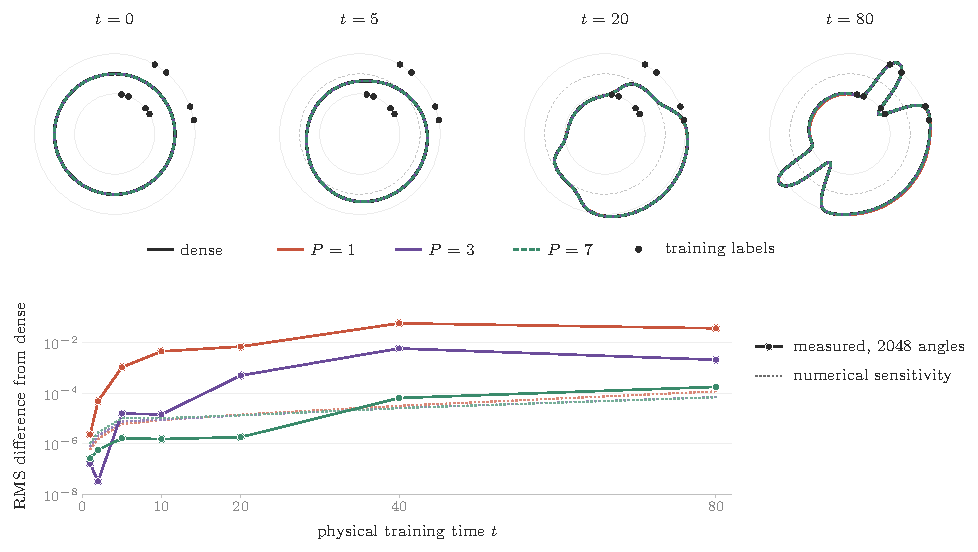
\includegraphics[width=\textwidth]{figures/trajectory.pdf}
 \caption{\textbf{Learning at common physical times.} Paired-label task, two
 hidden tanh layers, width $2048$: saved functions of dense training and of
 response memory at orders $q=1,3,7$ at the same physical times $t=0,5,20,80$.
 Radius is $3+f(\theta)$, the dashed ring marks $f=0$ and the light rings
 $f=\pm1$; black dots are training labels.  The RMS discrepancies at all $39$
 shared times are in \Cref{fig:trajectory-rms}.}
 \label{fig:trajectory}
\end{figure}

\FloatBarrier
\paragraph{Fitted functions across tasks.}
With eight labelled points on a circle, many functions fit the labels, so
agreement at training points says little. We compare the selected function
on $8192$ angles for five tasks with alternating labels, clustered points and
large unlabelled arcs. \Cref{fig:deep} displays the three-hidden-layer results;
the two-hidden-layer gallery is in \Cref{app:circle-gallery}.
The same initialization is used within each task and architecture.
A supplementary four-hidden-layer ReLU example on the sphere appears in
\Cref{app:sphere-endpoints}.

\begin{figure}[!tp]
 \centering
 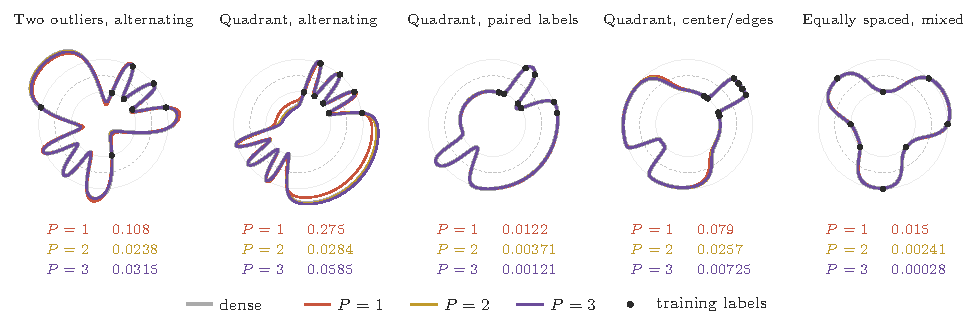
\includegraphics[width=\textwidth]{figures/circles_deep.pdf}
 \caption{\textbf{The fitted function across five tasks.} Three hidden tanh
 layers, width $4096$, and memory orders $q=1,2,3$, at each model's training-MSE
 $10^{-3}$ endpoint. Angle represents input direction; radius is $3+f(\theta)$,
 the dashed ring marks $f=0$ and the light rings $f=\pm1$.
 The thick grey curve is dense training, coloured curves are response memory,
 and black dots are training labels. The numbers under each panel are RMS
 differences from dense on $8192$ uniform circle points.}
 \label{fig:deep}
\end{figure}

In two hidden layers (\Cref{fig:shallow}, \Cref{tab:circle} in \Cref{app:circle-gallery}),
the fitted-function discrepancy falls by 1.5--3 orders
of magnitude from $q=1$ to $q=7$ on every task. In three hidden layers, $q=2$
and $q=3$ have RMS differences below $0.06$ on all five tasks, and below
$0.01$ on three. Order is not monotone at these small values: $q=2$ beats
$q=3$ on both alternating tasks; the observed numerical sensitivity is two
orders of magnitude below these differences, and no power law is fitted
(\Cref{fig:order}, \Cref{app:supp-figs}).  The hidden features move
substantially: the \emph{absolute} activation RMS
changes from initialization are $0.35$--$0.65$, $0.38$--$0.74$ and
$0.46$--$0.68$ in the three layers, across the 20 finest dense and closure runs.
The moving state at $q=3$ is about $3$\,MiB against $256$\,MiB for the dense
learned matrices; retained initialized matrices are additional.

Frozen dictionaries built at initialization are a different alternative:
on the outlier task they reach RMS $0.55$--$1.38$ with about 45 vectors,
against $0.073$ for 48 response moments. Together with the factor control that
follows, this motivates both parts of the method: evolving response directions and
an evolution law derived from the network's own history.

\FloatBarrier

\paragraph{Capturing the learned function requires the right dynamics.}
\Cref{fig:samerank} compares dense training with its full initialization-frozen
empirical tangent kernel, directly trained factors, and response memory.
All four fit the training labels to MSE approximately $0.001$, yet select
different functions between those labels. On the alternating-label quadrant
task, the frozen kernel has whole-circle RMS discrepancy $171.03$ from dense,
the two factor seeds have discrepancies $0.6766$ and $1.5413$, and memory at
$q=3$ has discrepancy $0.04561$. The kernel includes every parameter block with
the canonical mobilities; its construction and all five task comparisons are
given in \Cref{app:factors,fig:controls-gallery}.

Both response memory and directly trained factors retain the same $W_0^{(2)}$
and have evolving low-rank learned corrections. Their dynamics differ:
ordinary Euclidean factor gradient flow does not induce canonical matrix
gradient flow. \Cref{fig:samerank-summary} summarizes the comparison across tasks,
and \Cref{fig:factors} shows the fitted functions on the
paired-label task at correction rank bound $24$. Memory has whole-circle RMS
$0.00282$ from dense, against $0.375$ and $0.204$ for the two factor seeds.
Across all five tasks and three ranks, memory has smaller discrepancy in all
29 resolved fitted comparisons; one capped factor run is excluded. Twenty-eight
wins exceed a factor of two. Together, the controls show that the reproduced
predictor goes beyond the initial tangent model and this rank-matched factor
flow. They support the response-memory evolution law, without asserting a
universal comparison with kernels or low-rank algorithms.

\begin{figure}[!tp]
 \centering
 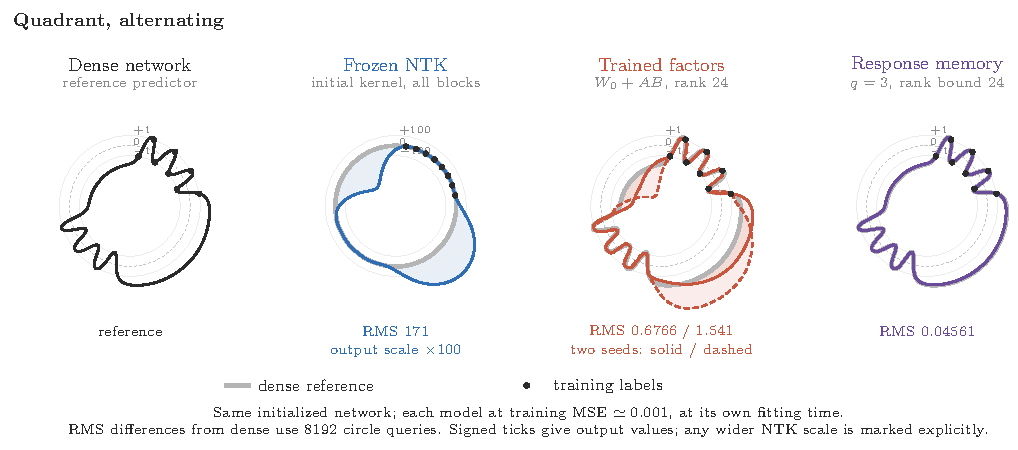
\includegraphics[width=\textwidth]{figures/learning_controls_quadrant_alternating.pdf}
 \caption{\textbf{Fitting the labels does not determine the learned function.}
 Alternating-label quadrant task, eight training inputs, two hidden tanh
 layers and width $2048$. From left: dense training, the full frozen empirical
 NTK, directly trained factors at rank $24$ (two seeds), and response memory
 at $q=3$ with rank bound $24$. All start from the same physical network and
 are evaluated at their own training-MSE $0.001$ endpoints. Gray curves show
 the dense reference in each panel; black dots are training labels.
 Angle is input direction and radius is linear in output. The NTK panel uses
 a $100$-times wider output scale, including its reference curve and labels;
 signed ticks show original output units. RMS values are unscaled discrepancies
 from dense over $8192$ circle queries, not errors against unseen labels.
 The complete five-task comparison appears in \Cref{fig:controls-gallery}.}
 \label{fig:samerank}
\end{figure}


\paragraph{MNIST.}
With 100 training images and width $4096$, held-out discrepancies are
$0.00325$, $0.00108$ and $0.00120$ for $q=1,2,3$, retaining the small
deterioration from $q=2$ to $q=3$; the predictions and their signed residuals
are shown in \Cref{fig:mnist} (\Cref{app:supp-figs}).
All models have identical test accuracy ($94.7\%$). With 1000 training images
and width $1024$, the discrepancies are $0.019$, $0.0019$ and $0.0012$, with
$97.5\%$ accuracy for dense, $q=2$ and $q=3$. Prediction fidelity and label
accuracy are separate observables.

\paragraph{Two clocks.}
The joint clock's better rate is asymptotic. At $q=5$ it improved some cases
(tanh alternating quadrant $0.0066\to0.0035$; GELU outliers $0.0020\to0.0010$)
and was much worse on another (GELU alternating quadrant $0.013\to1.00$, reduced
to $0.10$ by halving the step). Over an 82-configuration sweep, on the 65
configurations where dense and all orders fit, the joint clock's median
discrepancies were $0.031$, $0.013$ and $0.0066$ for $q=1,2,3$.

\section{Related work and comparison}
\label{sec:related}
We organize prior work by where it sits on the axis of the introduction: whether
it targets the specified deep nonlinear feature-learning flow and, when it
does, how its evolving state is represented.  \Cref{tab:axis} places one
representation from each description on that axis: what it stores and which
accuracy certificate addresses the specified target.  \Cref{sec:size} gives
our all-time trade-off; \Cref{app:size} details the additional hypotheses
needed to compare numerical solvers at a common tolerance.
\begin{table}[t]
\centering
\small
\renewcommand{\arraystretch}{1.18}
\caption{Where descriptions retain the evolving state.  Counts are per
hidden layer, omitting fixed sources and common outer weights; $N$ is the
number of retained training times.  Error claims must refer to the same
deep feature-learning target and horizon before their exponents can be
compared.  The last column records the available scope rather than
transferring a theorem from a different scaling.}
\label{tab:axis}
\begin{tabular}{@{}p{0.27\textwidth}p{0.20\textwidth}p{0.46\textwidth}@{}}
\toprule
Description & Moving state & Accuracy relative to the specified flow\\
\midrule
Deep linear; shallow mean field; frozen NTK
& Model dependent
& Change at least one of depth, nonlinearity or feature learning.\\
\midrule
Canonical dense network
& $n^2$
& All-time convergence as $n\to\infty$ in our small-label regime; no numerical width rate here.\\
Stored update histories
& $mnN$
& Exact representation of the chosen discrete updates; continuous-time error requires a numerical estimate.\\
Tensor Programs
& Representation dependent
& Fixed-program population laws; a solver and its numerical error must be specified.\\
Two-time DMFT solver
& $m^2N^2$ kernels
& Path sampling, time discretization and self-consistency errors require separate control.\\
Tangent hierarchy through $q$
& $\sum_{j<q}m^j$
& Published width/horizon estimate is in a different scaling; a matched hierarchy requires its own tail and stability bound.\\
\midrule
Response memory, speed clock
& $mnq$
& All-time $\omega(q)+o_{\Pr}(1)$ in \Cref{thm:alltime}; $\omega(q)=q^{-2+o(1)}$.\\
Response memory, joint clock
& $mnq+q^2$
& $O_{n,T}(q^{-2})$ on compact horizons (\Cref{thm:new}).\\
\bottomrule
\end{tabular}
\end{table}

\paragraph{Off the axis: descriptions that give up one property.}
Exact solutions of deep linear networks keep depth and feature learning but not
nonlinearity \citep{saxe2014exact}; their infinite-width limit is a gradient
flow on $\ell^2$ operators added to the frozen initialization
\citep{chizat2024linear}, the cleanest example of an operator description.
Wasserstein and mean-field limits describe one-hidden-layer networks as the
gradient flow of a measure over neurons
\citep{chizat2018global,mei2018meanfield,sirignano2019lln}; they keep nonlinear
feature learning but not depth.  The neural tangent kernel and lazy training
keep depth and nonlinearity but freeze the features, reducing training to a
fixed kernel \citep{jacot2018ntk,lee2019wide,chizat2019lazy}.  Each is simple
because of what it sacrifices, and each is exact about a different object.
These regime changes can leave a discrepancy that increasing width does not
remove.  This concerns the learning dynamics, not whether a shallow or kernel
model can represent a particular fitted function.

\paragraph{On the axis, paying in history.}
Tensor Programs~IV proves feature-learning limits at each fixed number of steps,
with a recursion that includes variables indexed by every earlier step
\citep{yang2021tensor}.  Feature-learning DMFT evolves two-time activation,
gradient and response kernels, with memory quadratic and time cubic in the
number of time points \citep{bordelon2022dmft}, and its finite-width extension
adds perturbative fluctuations \citep{bordelon2023finite}.  Direct two-time
storage is smaller than dense $O(n^2)$ weight storage per layer when the
number of samples times the number of time steps is well below the width.  Runtime additionally depends on sampled
single-site paths and self-consistency sweeps (\Cref{app:comparison-dmft}).
Multilayer mean-field theory and Neural Feature Flow evolve fields on neuronal
ensembles \citep{nguyen2023rigorous,fang2020features}.  These keep all three
properties within their respective parameterizations.  They compress width: DMFT, for
instance, has kernel state independent of the number of neurons.  Direct
history solvers retain time-indexed state; field descriptions instead retain
functions on population spaces.  Their representation and approximation
costs must be specified separately.
Our result is complementary: it keeps the neurons and compresses time.

\paragraph{On the axis, paying in tuples of samples.}
The Neural Tangent Hierarchy \citep{huang2020nth} evolves the outputs together
with the tangent kernels of order $2,\dots,q$, the $j$-th a function of $j$
training points, and closes by freezing the top kernel.  The hierarchy is an
exact identity in any parametrization, and above order two it captures feature
learning; the neural tangent kernel is its lowest truncation.  What it pays is
combinatorial in the samples: the moving state through order $q$ is
$\sum_{j=1}^{q-1}m^j\sim m^{q-1}$ scalars beneath a frozen tensor of $m^q$
entries (a direct count rather than a statement of that work), against a state
linear in $m$ here.  Its published guarantee uses width-suppressed higher
kernels: for even $q$ it gives an $n^{-q/2}$ factor multiplied by
time-dependent terms, on
a width-dependent horizon and under specified data and regularity assumptions.
Those estimates cannot simply be transferred to the present scaling, where
feature and kernel evolution can remain order one.  The matched hierarchy
still captures feature learning, but its truncation error must be controlled
through higher-kernel growth (\Cref{app:comparison-nth}).
Response memory instead controls the learned parameter trajectory and
whole-input prediction in \Cref{thm:alltime}, with state linear in $m$ and
$q$.  NTH's higher orders do capture feature learning; the issue in a
quantitative comparison is their tail in the same parameterization.

\paragraph{Memory and low rank.}
HiPPO provides online Legendre projection of a given signal \citep{gu2020hippo};
we apply it to endogenous, coupled training histories and prove stability of the
resulting feedback loop.  Low-rank training methods constrain the learned
increment to evolving factors \citep{zhao2023inrank}; response-memory factors are
causal summaries of the actual forward and backward histories, and a directly
trained factorization of matched rank performs far worse
(\Cref{sec:experiments}).

The comparison is therefore between representations and their certificates.
The proved improvement here is the all-time compression in
\Cref{cor:compression}.  A numerical ranking by powers of an accuracy
tolerance additionally needs width, discretization and stability rates for
each implementation; \Cref{app:size} states those obligations explicitly.

\section{Discussion: toward an idealized model of learning}

We asked whether the limiting process of deep feature learning can be
approximated by a smaller evolving state.  The central result gives a
constructive answer in a canonical small-label regime.  Each neuron remembers
finitely many paired response moments, and these memories evolve with the
network they reconstruct.  The resulting approximation follows the whole
training trajectory and its selected test function.  Any diverging sublinear
order reaches the dense population predictor with a vanishing fraction of
the dense learned state.

The loss-decay result is part of this mechanism.  Fitting is established for
every order before comparison with the dense model: it bounds the total
learning activity, keeps the readout-feature Gram nondegenerate, and makes
all-time error control possible.  The role of small labels can also be
expressed as a bound on feature-learning strength through the exact
rescaling in \Cref{cor:damped}.  This clarifies the regime without replacing
the canonical theorem by a different training algorithm.

The next questions are quantitative width concentration, a unique
fixed-order population moment law, and comparable all-time bounds when
feature movement is no longer small.  The current theorem requires zero
readout, a positive initial feature-Gram gap and smooth gates; exact ReLU
is outside its activation class.  Sample dependence remains linear, so a
continuum of training inputs needs a further representation.  Finally,
the initialized random operator remains a fixed dense environment:
compressing that environment while preserving its forward and adjoint reuse
is a different problem.  These questions concern the remaining parts of
the learning state; the response history itself already admits an
autonomous, quantitatively controlled compression.

\begin{thebibliography}{15}
\providecommand{\natexlab}[1]{#1}
\providecommand{\url}[1]{\texttt{#1}}
\expandafter\ifx\csname urlstyle\endcsname\relax
  \providecommand{\doi}[1]{doi: #1}\else
  \providecommand{\doi}{doi: \begingroup \urlstyle{rm}\Url}\fi

\bibitem[Bordelon and Pehlevan(2022)]{bordelon2022dmft}
Blake Bordelon and Cengiz Pehlevan.
\newblock Self-consistent dynamical field theory of kernel evolution in wide
  neural networks, 2022.
\newblock URL \url{https://arxiv.org/abs/2205.09653}.

\bibitem[Bordelon and Pehlevan(2023)]{bordelon2023finite}
Blake Bordelon and Cengiz Pehlevan.
\newblock Dynamics of finite width kernel and prediction fluctuations in mean
  field neural networks, 2023.
\newblock URL \url{https://arxiv.org/abs/2304.03408}.

\bibitem[Chizat and Bach(2018)]{chizat2018global}
L{\'e}na{\"i}c Chizat and Francis Bach.
\newblock On the global convergence of gradient descent for over-parameterized
  models using optimal transport.
\newblock In \emph{Advances in Neural Information Processing Systems},
  volume~31, 2018.

\bibitem[Chizat et~al.(2024)Chizat, Colombo, Fern\'andez-Real, and
  Figalli]{chizat2024linear}
L{\'e}na{\"i}c Chizat, Maria Colombo, Xavier Fern\'andez-Real, and Alessio
  Figalli.
\newblock Infinite-width limit of deep linear neural networks.
\newblock \emph{Communications on Pure and Applied Mathematics}, 2024.
\newblock \doi{10.1002/cpa.22200}.

\bibitem[Chizat et~al.(2019)Chizat, Oyallon, and Bach]{chizat2019lazy}
L{\'e}na{\"i}c Chizat, Edouard Oyallon, and Francis Bach.
\newblock On lazy training in differentiable programming.
\newblock In \emph{Advances in Neural Information Processing Systems},
  volume~32, 2019.

\bibitem[Fang et~al.(2020)Fang, Lee, Yang, and Zhang]{fang2020features}
Cong Fang, Jason~D. Lee, Pengkun Yang, and Tong Zhang.
\newblock Modeling from features: A mean-field framework for over-parameterized
  deep neural networks, 2020.
\newblock URL \url{https://arxiv.org/abs/2007.01452}.

\bibitem[Gu et~al.(2020)Gu, Dao, Ermon, Rudra, and R{\'e}]{gu2020hippo}
Albert Gu, Tri Dao, Stefano Ermon, Atri Rudra, and Christopher R{\'e}.
\newblock {HiPPO}: Recurrent memory with optimal polynomial projections, 2020.
\newblock URL \url{https://arxiv.org/abs/2008.07669}.

\bibitem[Huang and Yau(2020)]{huang2020nth}
Jiaoyang Huang and Horng-Tzer Yau.
\newblock Dynamics of deep neural networks and neural tangent hierarchy, 2020.
\newblock URL \url{https://arxiv.org/abs/1909.08156}.

\bibitem[Jacot et~al.(2018)Jacot, Gabriel, and Hongler]{jacot2018ntk}
Arthur Jacot, Franck Gabriel, and Cl{\'e}ment Hongler.
\newblock Neural tangent kernel: Convergence and generalization in neural
  networks, 2018.
\newblock URL \url{https://arxiv.org/abs/1806.07572}.

\bibitem[Lee et~al.(2019)Lee, Xiao, Schoenholz, Bahri, Novak, Sohl-Dickstein,
  and Pennington]{lee2019wide}
Jaehoon Lee, Lechao Xiao, Samuel~S. Schoenholz, Yasaman Bahri, Roman Novak,
  Jascha Sohl-Dickstein, and Jeffrey Pennington.
\newblock Wide neural networks of any depth evolve as linear models under
  gradient descent, 2019.
\newblock URL \url{https://arxiv.org/abs/1902.06720}.

\bibitem[Mei et~al.(2018)Mei, Montanari, and Nguyen]{mei2018meanfield}
Song Mei, Andrea Montanari, and Phan-Minh Nguyen.
\newblock A mean field view of the landscape of two-layer neural networks,
  2018.
\newblock URL \url{https://arxiv.org/abs/1804.06561}.

\bibitem[Nguyen and Pham(2023)]{nguyen2023rigorous}
Phan-Minh Nguyen and Huy~Tuan Pham.
\newblock A rigorous framework for the mean field limit of multilayer neural
  networks.
\newblock \emph{Mathematical Statistics and Learning}, 6\penalty0
  (3/4):\penalty0 201--357, 2023.
\newblock \doi{10.4171/MSL/42}.

\bibitem[Saxe et~al.(2014)Saxe, McClelland, and Ganguli]{saxe2014exact}
Andrew~M. Saxe, James~L. McClelland, and Surya Ganguli.
\newblock Exact solutions to the nonlinear dynamics of learning in deep linear
  neural networks.
\newblock In \emph{International Conference on Learning Representations}, 2014.

\bibitem[Sirignano and Spiliopoulos(2019)]{sirignano2019lln}
Justin Sirignano and Konstantinos Spiliopoulos.
\newblock Mean field analysis of neural networks: A law of large numbers, 2019.
\newblock URL \url{https://arxiv.org/abs/1805.01053}.

\bibitem[Yang and Hu(2021)]{yang2021tensor}
Greg Yang and Edward~J. Hu.
\newblock Tensor programs {IV}: Feature learning in infinite-width neural
  networks.
\newblock In \emph{Proceedings of the 38th International Conference on Machine
  Learning}, volume 139 of \emph{Proceedings of Machine Learning Research},
  pages 11727--11737. PMLR, 2021.
\newblock URL \url{https://proceedings.mlr.press/v139/yang21c.html}.

\bibitem[Zhao et~al.(2023)Zhao, Zhang, Chen, Sch{\"a}fer, and
  Anandkumar]{zhao2023inrank}
Jiawei Zhao, Yifei Zhang, Beidi Chen, Florian Sch{\"a}fer, and Anima
  Anandkumar.
\newblock {InRank}: Incremental low-rank learning, 2023.

\end{thebibliography}

\appendix

\section{Proof of the all-time theorem}
\label{app:proof-alltime}

We prove \Cref{thm:alltime} for layer-dependent activations.  Write
$g_\ell=(\phi_\ell)'$, and fix bounds
\[
 |\phi_\ell(0)|\le a,\qquad |g_\ell|\le s,\qquad
 |g_\ell(u)-g_\ell(v)|\le j|u-v|.
\]
All constants below may depend on these bounds, the fixed data and depth,
and the initial Gram margin.  They do not depend on $n,q$, or time.
Constants denoted by $C$ may increase from line to line.  For sample vectors
write $\|v\|_m^2=m^{-1}\sum_a v_a^2$, so $Y=\|y\|_m$.
Vector and matrix norms at finite width are ordinary Euclidean and
Frobenius norms; every normalization by $n$ is displayed.
The distance $d_n$ is the sum of scaled block norms in
\eqref{eq:normalized-distance}.  We first prove uniform fitting at every
order, then construct the dense Gaussian reference and transfer its carrier
tails, and finally use these tails to sharpen the closure error.

\subsection{Initialization and polynomial projection}

Let $v_a=x_a/\sqrt d$, $X=\max_a\|v_a\|_2$, and define the deterministic
uncentered feature covariances
\begin{align}
 Q^{(1)}_{ab}&=\E[\phi_1(G^\top v_a)\phi_1(G^\top v_b)],
       &&G\sim N(0,I_d),\nonumber\\
 Q^{(\ell)}_{ab}&=\E[\phi_\ell(Z_a)\phi_\ell(Z_b)],
       &&Z\sim N(0,Q^{(\ell-1)}),\quad\ell\ge2.
 \label{eq:at-initial-covariance}
\end{align}
Choose $\lambda>0$ with $Q^{(L)}/m\succeq2\lambda I_m$.
There are fixed $K_0,A_0,C_0$ such that the events
\begin{equation}
 \mathcal G_n=\left\{\begin{aligned}
 &
 \max_{\ell\ge2}\|W_0^{(\ell)}\|_{\rm op}\le K_0,\quad
 \max_a\frac{\|z_a^{(1)}(0)\|_2}{\sqrt n}\le A_0,\\
 &
 \frac{\|W_0^{(1)}\|_F}{\sqrt n}\le C_0,\quad
 \Gamma_w(0):=\frac{H_L(0)^\top H_L(0)}{mn}\succeq\lambda I_m
 \end{aligned}\right\}
 \label{eq:at-good-event}
\end{equation}
have probability tending to one.  Here $H_L$ has feature columns indexed
by the training samples.  Indeed, a $1/4$-net of the unit sphere has at
most $9^n$ points, and approximation of both vectors in a bilinear form
gives
\[
 \Pr\{\|W_0^{(\ell)}\|_{\rm op}>K_0\}
 \le2\,9^{2n}e^{-nK_0^2/8}\longrightarrow0
\]
for a sufficiently large fixed $K_0$.  The first-layer bounds follow from
the law of large numbers at fixed $d,m$.

For completeness, $H_\ell(0)^\top H_\ell(0)/n\to Q^{(\ell)}$ in
probability.  At the first layer this is a law of large numbers.
Conditionally on all previous layers, the rows of the next preactivation
matrix are independent $N(0,H_{\ell-1}^\top H_{\ell-1}/n)$ vectors.
Linear growth, $|\phi(u)|\le a+s|u|$, bounds each activation's Gaussian
fourth moment by $8a^4+24s^4Q_{aa}^2$.  Conditional Chebyshev therefore
bounds each covariance-entry error by $C(M)/(n\epsilon^2)$ whenever the
previous covariance has operator norm at most $M$.  Finally the map
$Q\mapsto\E[\phi(Q^{1/2}G)_a\phi(Q^{1/2}G)_b]$ is continuous,
including at singular $Q$: positive square roots converge, and a constant
multiple of $1+\|G\|_2^2$ is an integrable majorant on bounded covariance
sets.  Induction proves the assertion and hence the Gram part of
\eqref{eq:at-good-event}.

The input criterion stated with the theorem also follows directly.
If the nonzero $v_a$ are pairwise nonproportional and
$\sum_a c_a\phi_1(v_a^\top u)=0$ for all $u$, fix $a$ with
$c_a\ne0$.  For each $b\ne a$, choose $u_b\perp v_b$ with
$u_b\cdot v_a\ne0$.  Applying all $m-1$ finite differences in the
directions $t_bu_b$ eliminates every term but the $a$th, giving
\[
 \Delta_{s_1}\cdots\Delta_{s_{m-1}}\phi_1(t)=0
 \quad\text{for all }t,s_1,\ldots,s_{m-1}.
\]
Convolve with a smooth compactly supported approximate identity and
differentiate once in each $s_i$ at zero.  The mollified function is a
polynomial of degree at most $m-2$.  Its coefficients converge, by
interpolation at $m-1$ distinct points, so the original continuous
function is such a polynomial.  Thus a nonpolynomial first activation
makes the ridge functions independent.  A null quadratic form of
$Q^{(1)}$ would give a continuous ridge combination vanishing almost
everywhere under a full-support Gaussian, hence everywhere, and is
impossible.  If $Q\succ0$ and $\psi$ is continuous and nonconstant,
the identity $\sum_a c_a\psi(Z_a)=0$ for $Z\sim N(0,Q)$ likewise holds
everywhere; varying one coordinate shows $c_a=0$.  This propagates
positivity to all layers.  For $m=1$, a nonzero input and any nonconstant
first activation suffice.  Alternatively linearly independent inputs
give a positive first preactivation covariance, so any nonconstant
activation in every layer suffices.  A globally Lipschitz nonaffine
function is nonpolynomial.  These are sufficient criteria; the proof
below only needs the actual gap in \eqref{eq:at-initial-covariance}.

\begin{lemma}[Projection estimates used in the bootstrap]
\label{lem:at-projection}
Let $\Pi_q^A$ be orthogonal projection onto polynomials of degree below
$q$ in $L^2(0,A;\mathcal H)$, for a real Hilbert space $\mathcal H$.
For $u\in H^1(0,A;\mathcal H)$ and bounded measurable $b$,
\begin{align}
 \|(I-\Pi_q^A)u\|_{L^2}^2
 &\le\frac1{q(q+1)}\int_0^A\xi(A-\xi)\|u'(\xi)\|^2\dd\xi,
 \label{eq:at-weighted-tail}\\
 \|u(A)-(\Pi_q^Au)(A)\|
 &\le C\sqrt{A/q}\,\|u'\|_{L^2},&
 \|(\Pi_q^Ab)(A)\|&\le C\sqrt q\,\|b\|_{L^\infty}.
 \label{eq:at-endpoint}
\end{align}
If a history $u$ is fixed as its right endpoint grows, then
\begin{equation}
 \frac{\dd}{\dd A}\|(I-\Pi_q^A)u\|_{L^2(0,A)}^2
   =\|u(A)-(\Pi_q^Au)(A)\|^2
 \quad\text{for almost every }A.
 \label{eq:at-growing-energy}
\end{equation}
\end{lemma}
\begin{proof}
The normalized shifted Legendre modes $e_k$ satisfy
$-[\xi(A-\xi)e_k']'=k(k+1)e_k$.
Integration by parts and Bessel's inequality applied to the orthonormal
family $\sqrt{\xi(A-\xi)}e_k'/\sqrt{k(k+1)}$ give
\eqref{eq:at-weighted-tail}; the omitted modes have $k(k+1)\ge q(q+1)$.
Smooth approximation and an orthonormal expansion in $\mathcal H$ give
the stated generality.

On $[0,1]$ the endpoint kernel is
$K_q(u)=\sum_{k<q}(2k+1)p_k(u)=(p_q'(u)+p_{q-1}'(u))/2$.
Integration by parts yields
\[
 u(A)-(\Pi_q^Au)(A)
 =\frac12\int_0^A[p_q(\xi/A)+p_{q-1}(\xi/A)]u'(\xi)\dd\xi.
\]
The squared $L^2$ norm of this multiplier is
$A[(2q+1)^{-1}+(2q-1)^{-1}]/4$, proving the first endpoint bound.
For the other one it suffices to check $\int_0^1|K_q|\le C\sqrt q$.
Here is a short verification of the needed Legendre variation estimate.
For the ordinary Legendre polynomial $L_k$, set
$v(\theta)=\sqrt{\sin\theta}L_k(\cos\theta)$ and
$Q(\theta)=(k+1/2)^2+(4\sin^2\theta)^{-1}$.
The Legendre equation gives $v''+Qv=0$ and
$(v^2+(v')^2/Q)'=-Q'(v')^2/Q^2\ge0$ on $(0,\pi/2)$.
The values $L_{2r}(0)=(-1)^r\binom{2r}{r}/4^r$,
$L_{2r+1}(0)=0$, and $L_k'(0)=kL_{k-1}(0)$ show that this energy
at $\pi/2$ is at most $C/k$, using
$\binom{2r}{r}/4^r\le(r+1)^{-1/2}$.
Consequently, on $1/k\le\theta\le\pi/2$,
\[
 |\partial_\theta L_k(\cos\theta)|
 \le Ck^{-1/2}\{k(\sin\theta)^{-1/2}+(\sin\theta)^{-3/2}\}.
\]
Its integral is at most $C\sqrt k$.  On $[0,1/k]$, use
$|L_k'|\le k(k+1)/2$; this follows by summing
$L_{r+1}'-L_{r-1}'=(2r+1)L_r$ and $|L_r|\le1$ on $[-1,1]$.
The last bound follows, for example, by integrating
$(\cos\theta+i\sin\theta\cos\alpha)^r$ over $0\le\alpha\le\pi$.
Parity handles the other half.  Thus ${\rm Var}(L_k)\le C\sqrt k$,
which proves the kernel bound; $q=1$ is immediate.

Finally differentiate the minimum least-squares error on $[0,A]$.
The endpoint contributes the right side of \eqref{eq:at-growing-energy}.
The other term pairs the projection residual with the derivative of a
polynomial of degree below $q$ and vanishes by orthogonality.  Moment
coordinates and the invertible polynomial Gram matrix justify absolute
continuity of its coefficients on compact endpoint intervals.  This
argument only needs square-integrable histories for the last identity.
\end{proof}

\subsection{Fitting and continuation for every memory order}
\label{sec:at-fitting}

Fix an initialization in $\mathcal G_n$ and put $D_0=K_0+1$.
On the tube $\|W^{(\ell)}\|_{\rm op}<D_0$ for $\ell\ge2$ and
$\max_a\|z_a^{(1)}\|_2/\sqrt n<A_0+1$, define
\[
 M_1=a+s(A_0+1),\qquad M_\ell=a+sD_0M_{\ell-1}.
\]
Linear growth gives $\|h_a^{(\ell)}\|_2/\sqrt n\le M_\ell$.
Stop the local closure at first tube exit or activity
$S=4Y/\lambda$, reducing the eventual $Y_*$ so $S\le1$.
Since $w(0)=0$, the readout equation and backward recursion give
\begin{equation}
 \frac{\|w\|_2}{\sqrt n}\le2M_LS,
 \qquad \max_a\frac{\|\delta_a^{(\ell)}\|_2}{\sqrt n}
 \le\beta_\ell,\qquad
 \beta_L=2sM_LS,\quad\beta_\ell=sD_0\beta_{\ell+1}.
 \label{eq:at-rms}
\end{equation}
Thus every $\beta_\ell\le CY$.  In this subsection responses and
residuals belong to the closure, with hats suppressed.
Write $c_a=r_a/\rho$, $b_a^{(\ell)}=c_a\delta_a^{(\ell)}$,
and $A=\tau(t)\le1+S\le2$.  The forward prefix is constant and the
backward prefix is zero.  Projection contraction in the reconstruction gives
\begin{align}
 \|\widehat W^{(\ell)}-W_0^{(\ell)}\|_F
 &\le2M_{\ell-1}\beta_\ell\sqrt{(1+S)S}=O(Y^{3/2}),
 \label{eq:at-hidden-tube}\\
 \frac{\|\widehat W^{(1)}-W_0^{(1)}\|_F}{\sqrt n}
 &\le2X\beta_1S=O(Y^2).
 \label{eq:at-first-tube}
\end{align}
For the first inequality, the backward history's averaged squared norm
is at most $S\beta_\ell^2$, the forward one at most
$(1+S)M_{\ell-1}^2$, and
$\|uv^\top/n\|_F=(\|u\|_2/\sqrt n)(\|v\|_2/\sqrt n)$.
These bounds keep both tube boundaries strictly away for small $Y$.

Differentiating the reconstruction gives exactly
\begin{equation}
 \dot{\widehat\theta}=F(\widehat\theta)+E,\qquad E_1=E_w=0,
 \qquad E_\ell=\frac{2\rho}{mn}\sum_a
       (b_a^{(\ell)}-b_a^{(\ell)*})
       (h_a^{(\ell-1)}-h_a^{(\ell-1)*})^\top,
 \label{eq:at-defect}
\end{equation}
where stars denote projected endpoint values.  By
\eqref{eq:at-growing-energy}, zero initial projection errors, and
Cauchy--Schwarz, its accumulated absolute norm satisfies
\begin{equation}
 \int_0^t\|E_\ell(u)\|_F\dd u
 \le\frac2{mn}\sum_a
 \|(I-\Pi_q^A)b_a^{(\ell)}\|_{L^2(0,A)}
 \|(I-\Pi_q^A)h_a^{(\ell-1)}\|_{L^2(0,A)}.
 \label{eq:at-defect-product}
\end{equation}
This bounds total absolute velocity error, not just the error in a signed
history integral.

Set
\[
 Z_\ell(t)=\frac1{mn}\sum_a\int_0^{\tau(t)}
       \|\partial_\xi h_a^{(\ell)}\|_2^2\dd\xi.
\]
First $Z_1\le4Ss^2X^4\beta_1^2$.
Endpoint evaluation on degree-below-$q$ polynomials has norm
$q/\sqrt A$ because $\sum_{k<q}(2k+1)=q^2$.
The averaged backward endpoint error is consequently at most
$(q+1)\beta_\ell$ in normalized Euclidean norm.  Equations
\eqref{eq:at-weighted-tail}--\eqref{eq:at-defect} imply
\[
 \int_0^t\rho\|E_\ell/\rho\|_F^2\dd u
 \le2(1+S)^2\beta_\ell^2 Z_{\ell-1}(t).
\]
The clock chain rule is
\[
 \partial_\xi h_a^{(\ell)}=g_\ell(z_a^{(\ell)})\od
 \{(F_\ell/\rho+E_\ell/\rho)h_a^{(\ell-1)}
                   +\widehat W^{(\ell)}\partial_\xi h_a^{(\ell-1)}\}.
\]
As $\|F_\ell/\rho\|_F\le2\beta_\ell M_{\ell-1}$, the preceding
estimate proves inductively
\begin{align}
 Z_1&\le Z_1^*:=4Ss^2X^4\beta_1^2,\nonumber\\
 Z_\ell&\le Z_\ell^*:=3s^2\left[
 4S\beta_\ell^2M_{\ell-1}^4+
 \{D_0^2+2(1+S)^2\beta_\ell^2M_{\ell-1}^2\}Z_{\ell-1}^*\right]
 \le CY^3.
 \label{eq:at-forward-energy}
\end{align}
The factors $M_{\ell-1}^4$ and $M_{\ell-1}^2$ retain the contribution
of unbounded activation values.  No feature coordinate maximum is used.
The sharper endpoint bounds \eqref{eq:at-endpoint} now give forward
error at most $CY^{3/2}/\sqrt q$ and backward error at most
$CY\sqrt q$.  Their product in \eqref{eq:at-defect} yields
\begin{equation}
 e_E(t):=\sum_{\ell=2}^L\|E_\ell(t)\|_F
 \le CY^{5/2}\rho(t),\qquad
 \int_0^t e_E\dd u\le CY^3/q.
 \label{eq:at-relative-defect}
\end{equation}
The second estimate also follows from \eqref{eq:at-defect-product},
the $C Y^{3/2}/q$ forward tail and the $C Y^{3/2}$ backward history norm.

The tangent Gram in the residual equation is
\begin{equation}
 \Gamma_{ab}=\frac1m\left[
 \frac{(h_a^{(L)})^\top h_b^{(L)}}n+
 \frac{(\delta_a^{(1)})^\top\delta_b^{(1)}}n\,v_a^\top v_b+
 \sum_{\ell=2}^L
 \frac{(\delta_a^{(\ell)})^\top\delta_b^{(\ell)}}n
 \frac{(h_a^{(\ell-1)})^\top h_b^{(\ell-1)}}n\right].
 \label{eq:at-tangent-gram}
\end{equation}
Every summand is a parameter-gradient Gram, so $\Gamma\succeq\Gamma_w$.
Equation \eqref{eq:at-forward-energy} gives
\[
 \frac{\|H_L(t)-H_L(0)\|_F}{\sqrt{mn}}\le\sqrt{SZ_L^*},\qquad
 \|\Gamma_w(t)-\Gamma_w(0)\|_{\rm op}
       \le2M_L\sqrt{SZ_L^*}\le CY^2.
\]
After reducing $Y_*$, $\Gamma\succeq\lambda I/2$ and
$\|\Gamma\|_{\rm op}\le G_*$ on the stopped interval.
For the ordinary prediction Jacobian $J$,
$(JE)_a=\sum_{\ell\ge2}(\delta_a^{(\ell)})^\top E_\ell
h_a^{(\ell-1)}/n$, whence
\[
 \dot r=-2\Gamma r+JE,\qquad
 \|JE\|_m\le CY e_E\le CY^{7/2}\rho.
\]
Choose $Y_*$ so $CY_*^{7/2}\le\lambda/2$ and put $\kappa=\lambda/2$.
Taking the inner product with $r/\rho$ proves
\begin{equation}
 Y e^{-\Lambda t}\le\rho(t)\le Ye^{-\kappa t},\qquad
 \int_0^t\rho\dd u\le Y/\kappa=S/2,
 \label{eq:at-fitting}
\end{equation}
for a fixed finite $\Lambda$.  Thus the activity boundary is also excluded.

These arguments legitimately use the clock before its lower residual bound
has been proved.  The raw moment vector field is locally Lipschitz for
$\tau>0$, and all its velocities vanish at zero residual.  Local
uniqueness backwards from such an equilibrium excludes a first finite zero
on a nonstationary regular solution.  At fixed $n,q$, the physical bounds
above and the integral moment formulas bound the entire raw state in a
compact subset of $\tau>0$.  A finite maximal endpoint would therefore
extend.  This proves global existence, uniqueness and \eqref{eq:at-fitting}
for every $q\ge1$.  The dense flow has the same proof with $E=0$ and
hidden displacement at most $2S\beta_\ell M_{\ell-1}$.
All reductions of $Y_*$ impose finitely many inequalities whose left
sides vanish with $Y$; none involves width or order.

The update equations, \eqref{eq:at-relative-defect}, and forward chain rule
also give, for either path with its own residual,
\begin{align}
 \frac{\|\dot W^{(1)}\|_F}{\sqrt n}
  +\sum_{\ell=2}^L\|\dot W^{(\ell)}\|_F&\le CY\rho,
 &\frac{\|\dot w\|_2}{\sqrt n}&\le C\rho,\nonumber\\
 \max_{\ell,a}\frac{\|\dot z_a^{(\ell)}\|_2+
                      \|\dot h_a^{(\ell)}\|_2}{\sqrt n}&\le CY\rho,
 &\int_t^\infty\rho(u)\dd u&\le\rho(t)/\kappa.
 \label{eq:at-speeds}
\end{align}
Consequently physical parameters converge to finite interpolating limits.
The residual equation further gives
$\|\dot r\|_m\le C\rho$ and $\|\dot c\|_m\le C$.
When $Y=0$, both paths are stationary and all conclusions are immediate.

\subsection{The Gaussian reference and its finite-width transfer}
\label{sec:at-gaussian}

We give the Gaussian construction needed below, including the fixed
computation input.  Its purpose is to control full dense backward carriers,
including the trained readout.  All Gaussian bounds in this subsection
initially concern population reference computations; no Gaussian law for
the coordinates of a trained finite network is assumed.

\begin{lemma}[Fixed Gaussian computations]
\label{lem:at-fixed-program}
Consider a fixed finite list of typed vector instructions using independent
matrices with entries $N(0,1/n)$, both orientations of each same matrix,
independent identically distributed root tuples in each layer, deterministic
linear combinations, and $C^1$ coordinate maps with bounded first derivatives.
Root tuples in different layers are independent and have finite second
moments.  Every same-layer tuple has a deterministic limiting empirical law,
in probability in Wasserstein distance of order two.  Finite collections
of such programs sharing the arrays converge jointly.

The limiting forward and reverse actions of one initialized matrix are
\begin{equation}
 \mathscr W h=\xi_h+\sum_{s:\,\mathscr W^*u_s\ {\rm earlier}}
       u_s\,\E[\partial_{\zeta_s}h],\qquad
 \mathscr W^*u=\zeta_u+\sum_{r:\,\mathscr Wv_r\ {\rm earlier}}
       v_r\,\E[\partial_{\xi_r}u].
 \label{eq:at-source-rule}
\end{equation}
The centered Gaussian source covariances are
$\E[\xi_h\xi_v]=\E[hv]$ and $\E[\zeta_u\zeta_v]=\E[uv]$.
Distinct matrix/orientation source groups are independent of one another
and of the roots.  Each derivative is of the unrolled scalar expression
in named source coordinates, holding deterministic coefficients,
covariances and previously computed expectations fixed.
The statement allows singular source covariances.

The value conclusion also holds for continuous coordinate maps of at most
linear growth.  If roots are sub-Gaussian, activations are $C^2$ with
bounded first two derivatives, and the extra instructions are products
$b(z)p$ with bounded $C^1$ functions $b,b'$, these products also obey the
response rule \eqref{eq:at-source-rule}.
\end{lemma}
\begin{proof}
We record the conditioning argument to specify precisely the result being
used.  For one matrix $W$, collect previous constraints as $WV=Y$ and
$W^\top U=Q$.  Conditional on the computation transcript, query inputs
are fixed.  Revealing a new answer conditions only the queried matrix's
current Gaussian factor on one more linear constraint; coordinate
operations reveal no additional randomness.  Induction therefore leaves
the residual Gaussian factors for distinct matrices conditionally
independent.  When the two query Grams are invertible, Gaussian
orthogonal projection gives
\[
 W\mid\mathcal H\ \overset d=
 Y(V^\top V)^{-1}V^\top+
 U(U^\top U)^{-1}Q^\top P_{V^\perp}
 +P_{U^\perp}\widetilde W P_{V^\perp}.
\]
Indeed the displayed mean solves both constraints, using
$U^\top Y=Q^\top V$, and is Frobenius-orthogonal to their common
homogeneous solution space.  The last term is the Gaussian on that space.
For a new input $h$, write
$\alpha_n=(V^\top V)^{-1}V^\top h$ and $h_\perp=h-V\alpha_n$.
Then
\[
 Wh=Y\alpha_n+U\beta_n+
       \frac{\|h_\perp\|_2}{\sqrt n}P_{U^\perp}g,\qquad
 \beta_n=(U^\top U/n)^{-1}(Q^\top h_\perp/n),
\]
in conditional law, with independent $g\sim N(0,I_n)$.
If the limiting query Grams are positive definite, all coefficients
converge by induction.  The removed noise has conditional expected
normalized squared norm $\operatorname{rank}(U)/n$, and hence vanishes.
For bounded Lipschitz empirical tests, the remaining independent Gaussian
coordinates give conditional variance at most $4\|\psi\|_\infty^2/n$.
The conditional mean is an empirical continuous function of the old
tuple.  Second moments converge as well: the new Gaussian cross term
has variance $4\sigma^2\|m\|_2^2/n^2$ when the conditional mean is $m$,
and the Gaussian squared-norm average has variance $2/n$.
Thus weak convergence and second-moment convergence, equivalently
Wasserstein convergence of order two, propagate through a matrix call.
Lipschitz coordinate instructions propagate them directly.

To identify the mean, let $\alpha$ be the limiting regression coefficient
and $h_\perp=h-\sum_r\alpha_rv_r$.  Earlier reverse answers equal
$\zeta_s$ plus linear combinations of the $v_r$; their pairings with
$h_\perp$ are therefore $\E[\zeta_sh_\perp]$.
Gaussian integration by parts gives
\[
 \E[\zeta h_\perp]=(\E[u_su_t])_{st}\E[\nabla_\zeta h_\perp].
\]
After inserting the earlier forward decompositions in $Y\alpha$,
the terms containing $\alpha_r\E[\nabla_\zeta v_r]$ cancel.
The remaining response is $\sum_su_s\E[\partial_{\zeta_s}h]$.
The Gaussian part has variance $\E[h^2]$ and covariance $\E[hv_r]$
with each previous forward source.  Its fresh innovation is independent
of other source groups.  This proves \eqref{eq:at-source-rule};
interchanging the two orientations proves the reverse formula.

To remove the rank assumption, add a fresh independent input
$\epsilon\chi$ at each matrix call.  At fixed $\epsilon>0$ the squared
distance of the new query from the previous query span has limiting
value at least $\epsilon^2$: the new Gaussian squared residual tends
to one, and its cross term has conditional variance $O(1/n)$ on
bounded norm events.  All limiting query Grams are then positive definite.
On the common initialized-operator event and the event
$\|\chi\|_2/\sqrt n\le2$ for the finitely many added roots, finite
instruction induction gives
$\max_v\|v_n^\epsilon-v_n\|_2/\sqrt n\le C\epsilon$.
The scalar response construction is also continuous at $\epsilon=0$.
Its covariance matrices converge, so couple their source vectors by
$K_\epsilon^{1/2}G$.  Positive square roots are continuous even at
singular matrices: bounded subsequences of the roots have limits whose
square is $K$, and uniqueness of the positive root identifies every
limit.  At a fixed finite instruction, scalar values have a uniform
linear envelope and their first source derivatives are bounded when
earlier coefficients lie in a compact set.  Dominated convergence
therefore passes values, second moments and expected source derivatives
to zero noise, closing this finite induction.  Taking width first and
then $\epsilon\downarrow0$ proves the singular case.  This argument
uses no continuity of pseudoinverses.

For a continuous map $F$ with a linear envelope, $X_j\to X$ in $L^2$
implies $F(X_j)\to F(X)$ in $L^2$: compact uniform continuity gives
convergence in probability, and the common linear envelope supplies
uniform integrability.  Approximate $F$ by smooth compactly supported
maps with a common linear envelope.  Choose each current approximation
first, then the approximation tolerance for its finite input prefix
smaller than its error budget divided by that smooth map's Lipschitz
constant.  Matrix actions multiply same-array RMS errors by at most
$K_0$.  Finite induction therefore removes these approximations in both
the scalar and empirical laws; no uniform cutoff Lipschitz constant is
needed.

For the final response assertion, replace $b(z)p$ by
$b(z)\chi_R(p)$, where $\chi_R$ is a smooth clip with
$|\chi_R(p)|\le|p|$, $|\chi_R'|\le1$, converging locally in $C^1$ to
the identity.  The clipped coordinate maps have bounded derivatives.
In a fixed scalar program the values have a linear envelope in the finite
root/source list; their first source derivatives have a polynomial
envelope, since each differentiated product adds at most one carrier
factor.  Sub-Gaussian roots and finite Gaussian source lists have all
moments.  Covariance-square-root coupling and uniform integrability thus
pass the expected derivatives through the clips, one instruction at a
time.  The value limit agrees with the preceding continuous-map
extension.  The number of instructions is fixed throughout.
\end{proof}

The same-array operator inequality used in this proof constructs actual
population operators, rather than independent reverse maps.  Include a
countable family of all required finite programs, their finite unions,
rational linear combinations, smooth coordinate approximations, and
forward and reverse queries.  Their scalar laws are consistent, since
deleting unused instructions changes no finite-array node.  Realize their
countable joint laws, separately at each layer, and complete the generated
span in $L^2$.  The high-probability inequality
$\|W_0v\|_2/\sqrt n\le K_0\|v\|_2/\sqrt n$ passes to each finite generated
span by second-moment convergence, then to its completion.  Including
a countable dense family of bounded smooth functions of finite tuples
makes this completion the $L^2$ space of the generated sigma field.
The finite identity
$n^{-1}u^\top W_0v=n^{-1}(W_0^\top u)^\top v$ passes to these spans
and then by continuity, so the reverse action is exactly $W_0^*$.
Increments of a hidden operator will be Hilbert--Schmidt:
$(u\otimes v)h=u\E[vh]$ has
$\|u\otimes v\|_{\rm HS}=\|u\|_2\|v\|_2$, the counterpart of the
finite Frobenius identity.

\paragraph{Activity-stopped population programs.}
Initially assume the activations are $C^2$ with
$\|\phi_\ell'\|_\infty\le s$ and $\|\phi_\ell''\|_\infty\le j$.
Use upper-case $Z,H,P$ for population scalar fields, with
$P_a^{(L)}=w$, $P_a^{(\ell)}=(W^{(\ell+1)})^*\delta_a^{(\ell+1)}$,
and $\delta_a^{(\ell)}=g_\ell(Z_a^{(\ell)})P_a^{(\ell)}$.
For an Euler program with physical steps $h_k$, let
\[
 \rho_k=\|r_k\|_m,\qquad \alpha_k=h_k\rho_k,\qquad
 u_{a,k}=r_{a,k}/\rho_k .
\]
Freeze zero-residual nodes.  Otherwise $|u_{a,k}|\le\sqrt m$.
The update formulas in activity are
\begin{align}
 \Delta w_k&=-\frac{2\alpha_k}{m}\sum_a u_{a,k}H_{a,k}^{(L)},\nonumber\\
 \Delta W_k^{(1)}&=-\frac{2\alpha_k}{m}\sum_a
                  u_{a,k}\delta_{a,k}^{(1)}v_a^\top,\nonumber\\
 \Delta W_k^{(\ell)}&=-\frac{2\alpha_k}{m}\sum_a
                  u_{a,k}\delta_{a,k}^{(\ell)}\otimes H_{a,k}^{(\ell-1)}.
 \label{eq:at-pop-euler}
\end{align}
At any fixed population program all coefficients here are deterministic,
although calculated causally from earlier population expectations.
Thus Lemma~\ref{lem:at-fixed-program} applies with these coefficients
frozen in every source derivative.

Stop at activity $\sum_{k<j}\alpha_k\le S\le1$ and at the physical tube
used above.  The same linear-growth induction gives $\|H_a^{(\ell)}\|_2
\le M_\ell$, $\|w\|_2\le2M_LS$, and
$\|\delta_a^{(\ell)}\|_2\le C_\ell S$.
Summing the rank-one updates gives first-layer and hidden increments
at most $CS^2$.  Subtracting successive forward recursions then gives
\[
 \max_{\ell,a}\|H_a^{(\ell)}-H_a^{(\ell)}(0)\|_2\le CS^2,\qquad
 \|\Gamma_w-\Gamma_w(0)\|_{\rm op}\le CS^2.
\]
These estimates also hold at an affine Euler interpolation state, regarded
as one final fractional step.  There is therefore a fixed $S_b>0$ for
which every stopped state has strict tube margins and
\begin{equation}
 \Gamma\succeq\lambda I/2,\qquad \|\Gamma\|_{\rm op}\le G,\qquad
 \|F\|_{\rm sum}\le V\rho .
 \label{eq:at-pop-tube}
\end{equation}
Here the parameter norm is the sum of the $L^2$ first-layer and readout
norms and the Hilbert--Schmidt hidden-increment norms.  The residual is
also bounded by a fixed constant on this tube.

\paragraph{A response bound uniform in the number of steps.}
For each hidden initialized matrix, introduce its forward sources
$\xi_{a,k}^{(\ell)}$ and reverse sources $\zeta_{a,k}^{(\ell)}$.
Their within-group covariances are respectively
$\E[H_{a,k}^{(\ell-1)}H_{b,r}^{(\ell-1)}]$ and
$\E[\delta_{a,k}^{(\ell)}\delta_{b,r}^{(\ell)}]$.
Expanding the learned operators in \eqref{eq:at-pop-euler} and using
\eqref{eq:at-source-rule} gives
\begin{align}
 Z_{a,k}^{(\ell)}
 &=\xi_{a,k}^{(\ell)}
       +\sum_{b,r<k}\mathsf F_{ak,br}^{(\ell)}\delta_{b,r}^{(\ell)},
 &P_{a,k}^{(\ell-1)}
 &=\zeta_{a,k}^{(\ell)}
       +\sum_{b,r\le k}\mathsf D_{ak,br}^{(\ell)}H_{b,r}^{(\ell-1)},
 \label{eq:at-response-fields}\\
 \mathsf F_{ak,br}^{(\ell)}
 &=\mathsf C_{ak,br}^{(\ell)}
       -\frac{2\alpha_ru_{b,r}}m
          \E[H_{b,r}^{(\ell-1)}H_{a,k}^{(\ell-1)}],
 &\mathsf C_{ak,br}^{(\ell)}
 &=\E\frac{\partial H_{a,k}^{(\ell-1)}}{\partial\zeta_{b,r}^{(\ell)}},
 \nonumber\\
 \mathsf D_{ak,br}^{(\ell)}
 &=\mathsf A_{ak,br}^{(\ell)}
       -\mathbf1_{r<k}\frac{2\alpha_ru_{b,r}}m
          \E[\delta_{b,r}^{(\ell)}\delta_{a,k}^{(\ell)}],
 &\mathsf A_{ak,br}^{(\ell)}
 &=\E\frac{\partial\delta_{a,k}^{(\ell)}}{\partial\xi_{b,r}^{(\ell)}}.
 \nonumber
\end{align}
The root equations are the first-layer and readout recursions in
\eqref{eq:at-pop-euler}.  The training-memory coefficients are bounded
by $J\alpha_r/m$ for a fixed $J$, by the preceding RMS bounds.

For a scalar random variable let
$\mathcal N(U)=\sup_{p\ge2}\|U\|_p/\sqrt p$.
If $\mathcal N(U)\le B$, expansion of the exponential and
$r!\ge(r/e)^r$ give
$\E e^{U^2/(8eB^2)}\le4/3$, and hence
$\E e^{t|U|}\le(4/3)e^{2et^2B^2}$.
Jensen's inequality with weights $\alpha_r/(m\sum\alpha_r)$ therefore
gives, without temporal independence,
\begin{equation}
 \E\exp\left(t\sum_{r<k}\frac{\alpha_r}{m}
                         \sum_b|P_{b,r}^{(\ell)}|\right)
       \le\frac43 e^{2et^2S^2B^2}
 \quad\text{if all }\mathcal N(P_{b,r}^{(\ell)})\le B.
 \label{eq:at-weighted-exponential}
\end{equation}
We verify simultaneously the caps
\begin{equation}
 \sum_{b,r\le k}|\mathsf A_{ak,br}^{(\ell)}|\le\mathfrak a_\ell,
 \qquad
 |\mathsf C_{ak,br}^{(\ell)}|\le\mathfrak c_\ell\alpha_r/m,
 \qquad \mathcal N(H)\le B_H,\quad
 \mathcal N(P^{(\ell)})\le B_{P,\ell}.
 \label{eq:at-response-caps}
\end{equation}
Set $f_\ell=\mathfrak c_\ell+J$ for $\ell\ge2$, $f_1=1$,
$d_\ell=1+\mathfrak a_{\ell+1}$ for $\ell<L$, and $d_L=1$.
Choose $K\ge2$ depending only on the roots, source RMS bounds and
activation bounds, before choosing the response caps.  The field
recursions imply
\begin{align*}
 \mathcal N(H_{a,k}^{(1)})&\le K+KS\sup_{b,r<k}\mathcal N(P_{b,r}^{(1)}),\\
 \mathcal N(H_{a,k}^{(\ell)})&\le K+Kf_\ell S
                              \sup_{b,r<k}\mathcal N(P_{b,r}^{(\ell)}),\\
 \mathcal N(P_{a,k}^{(\ell)})&\le K+(\mathfrak a_{\ell+1}+JS)
                              \sup_{b,r\le k}\mathcal N(H_{b,r}^{(\ell)}),\\
 \mathcal N(w_k)&\le K+KS\sup_{b,r<k}\mathcal N(H_{b,r}^{(L)}).
\end{align*}
The first two inequalities use linear growth, and $\delta=g_\ell(Z)P$
uses only bounded slope.  Thus the forward fields must be bootstrapped
together with the full backward carriers.

Here are the derivative estimates that close this bootstrap.  Let $V_k$
be the maximum through time $k$ of the sum of absolute derivatives of
$Z_a^{(\ell)}$ with respect to its own forward slots.  Differentiating
\eqref{eq:at-response-fields}, the derivative row of $P_a^{(\ell)}$
is bounded by $C d_\ell V_k$; at the top use the readout update instead.
The product rule gives a row bound
$C(|P_a^{(\ell)}|+d_\ell)V_k$ for $\delta_a^{(\ell)}$.  Since the
forward memory uses earlier times only,
\[
 V_k\le1+Cf_\ell\sum_{r<k}\alpha_r
       \left(d_\ell+\frac1m\sum_b|P_{b,r}^{(\ell)}|\right)V_r.
\]
For a single backward source at $(b,r)$ let $D_k$ be the maximal
absolute derivative of the lower preactivation through time $k$.
It is zero for $k\le r$.  At the source time, differentiation of the
direct Gaussian in $P$ gives one pulse; inserting it in the first-layer
update or the next forward memory retains exactly $\alpha_r/m$.
All later derivatives consequently obey
\[
 D_k\le Cf_{\ell-1}\alpha_r/m+
 Cf_{\ell-1}\sum_{u<k}\alpha_u
       \left(d_{\ell-1}+\frac1m\sum_a|P_{a,u}^{(\ell-1)}|\right)D_u.
\]
Discrete Gronwall, \eqref{eq:at-weighted-exponential}, and
Cauchy--Schwarz for the terminal carrier factor yield
\begin{align}
 \sum_{b,r\le k}|\mathsf A_{ak,br}^{(\ell)}|
 &\le C(B_{P,\ell}+d_\ell)
       e^{Cf_\ell Sd_\ell+Cf_\ell^2S^2B_{P,\ell}^2},\nonumber\\
 \frac{|\mathsf C_{ak,br}^{(\ell)}|}{\alpha_r/m}
 &\le Cf_{\ell-1}
       e^{Cf_{\ell-1}Sd_{\ell-1}
                          +Cf_{\ell-1}^2S^2B_{P,\ell-1}^2}.
 \label{eq:at-cap-improvement}
\end{align}
Fix one sufficiently large $C$ in these inequalities independently of
the caps.  Choose, in order,
\[
 \mathfrak c_2=4C,\qquad
 \mathfrak c_\ell=4C(\mathfrak c_{\ell-1}+J)\quad(\ell>2),
 \qquad
 \mathfrak a_L=4C(2K+1),\qquad
 \mathfrak a_\ell=4C(4K+1)(1+\mathfrak a_{\ell+1}) .
\]
The $\mathfrak c$ caps are selected from bottom to top, the
$\mathfrak a$ caps from top to bottom.  Set
$B_H=B_{P,L}=2K$ and
$B_{P,\ell}=4K(1+\mathfrak a_{\ell+1})$ for $\ell<L$.
All these constants are now fixed.  Choose $S_r>0$ so $JS_r\le1$,
$2KS_r\le1$, $f_\ell S_rB_{P,\ell}\le1$, and every exponent in
\eqref{eq:at-cap-improvement} is at most $\log2$.
The field recursions preserve their caps, and the response estimates
improve theirs by a factor of two.

This is a chronological induction, not an assumption on future fields.
At node $k$, the first layer and readout use only earlier nodes.
Construct current forwards from bottom to top: each current
$\mathsf C^{(\ell)}$ uses the already constructed lower field and past
lower carriers, after which $H^{(\ell)}$ uses only past same-layer
carriers.  Construct current backwards from top to bottom: the current
upper response supplies the next carrier, and its derivative row supplies
the next $\mathsf A$.  At $k=0$ forward memory is empty and the readout
is the zero root.  This starts the induction.  A fractional last Euler
step changes only its nonnegative activity weight.  We have proved, for
every program stopped at $S\le\min(S_b,S_r)$, including every affine
interpolation state,
\begin{equation}
 \max_{\ell,a}\E e^{c|U_a^{(\ell)}|^2}\le C,
 \qquad U\in\{Z,H,P,\delta\}.
 \label{eq:at-pop-gaussian}
\end{equation}
The constants are independent of physical duration and number of steps.

\paragraph{Excluding the stop and constructing the strong flow.}
On the parameter tube, forward subtraction costs $Cd$ in the parameter
distance.  For a reference carrier $P_*$, the only difficult backward
product is controlled by
\begin{equation}
 \|[g_\ell(Z)-g_\ell(Z_*)]P_*\|_2
 \le jR\|Z-Z_*\|_2+2s\|P_*\mathbf1_{\{|P_*|>R\}}\|_2 .
 \label{eq:at-reference-cutoff}
\end{equation}
The remaining backward difference is propagated by bounded operators
and bounded gates, so new cutoff contributions add through fixed depth.
The rank-one identity and \eqref{eq:at-pop-gaussian} therefore give,
for the prediction differential $J$ from the mobility Hilbert space to
sample RMS,
\begin{equation}
 \|J(\vartheta)-J(\theta_*)\|
 \le C\{(1+R)d(\vartheta,\theta_*)+e^{-cR^2}\}.
 \label{eq:at-jacobian-modulus}
\end{equation}
Only the reference node needs tails.  The scalar prediction is
continuously differentiable in these parameter spaces.  To check the
possibly unbounded multiplier explicitly, its scalar Taylor remainder
satisfies, for a fixed $P\in L^2$,
\[
 |\E[P\{\phi(Z+h)-\phi(Z)-g(Z)h\}]|
 \le \tfrac12jR\|h\|_2^2+
       2s\|P\mathbf1_{\{|P|>R\}}\|_2\|h\|_2=o(\|h\|_2).
\]
First send $h$ to zero at fixed $R$, then $R$ to infinity.
Forward subtraction and descending this weighted scalar expansion give
the displayed Jacobian; bounded-multiplier continuity proves its
continuity.  This does not assume that the full activation map is
Fréchet differentiable from $L^2$ to $L^2$.

An Euler segment has parameter length at most $Vh_k\rho_k$.
Integrating the prediction differential on that segment and using
\eqref{eq:at-jacobian-modulus} gives
\[
 r_{k+1}=(I-2h_k\Gamma_k)r_k+e_k,\qquad
 \|e_k\|_m\le h_k\rho_k\omega(h_k),\qquad
 \omega(h)=C\inf_{R\ge1}\{(1+R)h+e^{-cR^2}\}\longrightarrow0.
\]
For sufficiently small maximal physical step,
\eqref{eq:at-pop-tube} implies
\[
 \rho_{k+1}\le(1-\lambda h_k/2)\rho_k,\qquad
 \sum_{k<j}h_k\rho_k\le2Y/\lambda.
\]
Choose $S=4Y/\lambda$ and reduce $Y_*$ so
$S\le\min(S_b,S_r)$.
The first attainment of this activity cap, even by a shortened final
step, contradicts the strict factor-two margin.  The physical tube
already has a strict margin.  These deterministic Euler programs
therefore extend through every prescribed physical horizon.

Put countably many refining programs on all integer horizons on the
common generated spaces above.  The vector-field version of
\eqref{eq:at-jacobian-modulus} follows from backward subtraction and
rank-one update subtraction.  Comparing two Euler interpolants on
$[0,T]$, with maximal steps $h,h'$, gives
\begin{equation}
 \sup_{t\le T}d(\theta^h(t),\theta^{h'}(t))
 \le C_Te^{C(1+R)T}
       \{(1+R)(h+h')+e^{-cR^2}\}.
 \label{eq:at-pop-cauchy}
\end{equation}
The same argument holds in the Hilbert--Schmidt increment norm because
$\|u\otimes v-u'\otimes v'\|_{\rm HS}
\le\|u-u'\|_2\|v\|_2+\|u'\|_2\|v-v'\|_2$.
First send the meshes to zero at fixed $R$, then $R$ to infinity.
Since $e^{CRT-cR^2}\to0$, completeness gives a uniform strong limit.
For the passage through backward gates, if $Z_i\to Z$ in probability
and $P_i\to P$ in $L^2$, split
$g(Z_i)P_i-g(Z)P$ into $g(Z_i)(P_i-P)$ and
$[g(Z_i)-g(Z)]P$.  The former converges by boundedness of $g$;
truncate the single integrable variable $P^2$ to prove convergence of
the latter.  Thus the vector field is continuous, and the Euler
integral equations pass to the limit.

The same reference comparison against this constructed solution proves
uniqueness: the discrepancy of two solutions is at most
$C_Te^{CRT-cR^2}$ for every $R$, hence zero, up to any first tube exit.
Equality to the constructed path excludes that exit.  Solutions from
different horizons agree on overlaps.  The Gram gap survives the limit,
and the exact residual equation $\dot r=-2\Gamma r$ gives exponential
decay and finite total parameter variation, with the constants in
\eqref{eq:at-fitting}--\eqref{eq:at-speeds} decreased or enlarged if
necessary.  The limit at infinite physical time is an interpolating
parameter state.  At each time, $L^2$ convergence and Fatou pass
\eqref{eq:at-pop-gaussian} to the solution; the constants are common to
all times.  Applying the same reasoning at the parameter limit includes
$t=\infty$.  The assertion bounds time marginals; it places no time
supremum inside the exponential.

Finally remove classical second differentiability.  Compactly supported
mollification gives
$\|\phi_{\ell,\epsilon}-\phi_\ell\|_\infty\le Cs\epsilon$,
$\|g_{\ell,\epsilon}-g_\ell\|_\infty\le Cj\epsilon$,
$\|g_{\ell,\epsilon}\|_\infty\le s$ and
$\|g_{\ell,\epsilon}'\|_\infty\le j$.
The value at zero is uniformly bounded.  All response caps and activity
thresholds are therefore common to sufficiently small smoothings.
The initialization recursion \eqref{eq:at-initial-covariance} is continuous
under these uniform activation perturbations, so its positive Gram margin
also persists, after decreasing the common margin once.
The comparison \eqref{eq:at-pop-cauchy} between different smoothings
has the additional term $C(1+R)(\epsilon+\epsilon')$ inside braces.
After constructing each smoothed flow, take smoothing scales to zero at
fixed $R$ and then $R$ to infinity.  This gives the strong solution for
the stated $C^1$ activations with Lipschitz derivatives, with the same
uniqueness and Gaussian bounds.

\begin{lemma}[Dense carrier transfer]
\label{lem:at-gaussian-tail}
On the events \eqref{eq:at-good-event}, let
$k_{a,D}^{(L)}=w_D$ and
$k_{a,D}^{(\ell)}=(W_D^{(\ell+1)})^\top\delta_{a,D}^{(\ell+1)}$
for $\ell<L$.  Define
\[
 H_n(M,t)=\sum_{\ell=1}^L\max_a
       \frac{\|k_{a,D}^{(\ell)}(t)
           \mathbf1_{\{|k_{a,D}^{(\ell)}(t)|>M\}}\|_2}{\sqrt n},
 \qquad Z_n(M)=\int_0^\infty\rho_D(t)H_n(M,t)\dd t,
\]
and set $Z_n(M)=0$ off $\mathcal G_n$.  There are constants $c,C>0$
and dense-only random variables $a_n\ge0$, with $a_n\to0$ in
probability, such that, simultaneously for all integer $M\ge1$,
\begin{equation}
 Z_n(M)\le Ce^{-cM^2}+a_n.
 \label{eq:at-dense-tail}
\end{equation}
On each finite physical horizon, dense finite-width predictions on any
fixed finite list of training or passive test inputs converge in probability,
uniformly in time, to the predictions of the unique strong population
flow just constructed.
\end{lemma}
\begin{proof}
Fix a finite horizon $T$, a reference cutoff $R$, and a finite population
Euler mesh.  Evaluate its expanded initialized-matrix calls on the actual
finite Gaussian arrays, keeping every residual and scalar contraction
equal to its deterministic population value.  This is a fixed finite
program to which Lemma~\ref{lem:at-fixed-program} applies.
Reconstruct finite proxy parameters by the rank-one updates with those
oracle vectors.  For example a proxy action on an oracle feature differs
from its prescribed action by a finite sum of terms of the form
\[
 -\frac{2\alpha_ru_{b,r}}m\,\delta_{b,r}^{(\ell)}
 \left\{\frac{(h_{b,r}^{(\ell-1)})^\top h_{a,k}^{(\ell-1)}}n
              -\E[H_{b,r}^{(\ell-1)}H_{a,k}^{(\ell-1)}]\right\}.
\]
Each brace converges to zero; all involved vector RMS norms are bounded
in probability.  Forward recomputation is therefore consistent.
For backward recomputation use \eqref{eq:at-reference-cutoff} against
the oracle carriers.  Continuous quadratic-growth cutoff measurements
of their joint empirical laws converge by the lemma.  At fixed cutoff
the consistency errors vanish, and the limiting cutoff tails are
$Ce^{-cR^2}$ by \eqref{eq:at-pop-gaussian}.  Sending that cutoff to
infinity proves RMS consistency of the recomputed backward fields,
residuals, and vector field.

Compare actual finite dense gradient flow to this proxy interpolant,
stopping it only if it leaves a slightly larger physical tube.
The identical reference inequality and integral comparison give
\[
 \sup_{t\le T}d_n(\theta_{n,D}(t),\theta_{n,\mathrm{proxy}}^h(t))
 \le C_Te^{C(1+R)T}
       \{(1+R)h+e^{-cR^2}+o_{\mathbb P}(1)\}.
\]
The last term is at fixed $h,R$.  The proof uses empirical tails only
of fixed-program reference nodes.  Taking width to infinity at fixed
$h,R$, then $h$ to zero, then $R$ to infinity makes the error smaller
than the exit margin and excludes the stop.  Combining this with
\eqref{eq:at-pop-cauchy} proves the compact-time observable convergence.
For the original $C^{1,1}$ activations insert a fixed smooth reference
program and its $C(1+R)\epsilon$ comparison error, taking its smoothing
scale to zero before the final $R$ limit.  Passive test inputs require
only finitely many extra forward queries and first-layer root coordinates;
they change no training update.  They are therefore covered by exactly
the same fixed-program and comparison arguments.

We spell out how this yields actual dense carrier tails.  For fixed
$M$, use the continuous 1-Lipschitz function
$g_M(v)=(|v|-M)_+$, with
$|v|\mathbf1_{\{|v|>2M\}}\le2g_M(v)$.
Its normalized Euclidean norm changes by at most the RMS change in
the carrier.  Fixed-program convergence transfers its squared norm at
every reference node.  A finite time grid, the uniform parameter-speed
bound, and \eqref{eq:at-reference-cutoff} against these reference nodes
control the interpolation error.  First choose the grid and a comparison
cutoff, let width tend to infinity at that fixed program, then refine
the grid and remove the comparison cutoff.  The population Gaussian
bound implies a limiting carrier cutoff norm at most $Ce^{-cM^2}$,
after halving $M$ and changing $c$.  Prediction convergence also
transfers the residual factor.  We conclude that for every fixed
$M\ge1$ and $\epsilon>0$,
\[
 \Pr\left\{\int_0^T\rho_D(t)H_n(M,t)\dd t
                   >Ce^{-cM^2}+\epsilon\right\}\longrightarrow0.
\]
The constant is independent of $T$: population carrier tails are uniform
in time and total residual activity is bounded.
On $\mathcal G_n$, finite dense RMS bounds imply $H_n(M,t)\le C$,
and \eqref{eq:at-fitting} gives
$\int_T^\infty\rho_DH_n\dd t\le Ce^{-\kappa T}$
uniformly in $n,M$.  Choosing $T$ after the error tolerance but before
the width limit proves
\[
 \Pr\{Z_n(M)>Ce^{-cM^2}+\epsilon\}\longrightarrow0
 \quad\text{for every fixed }M\ge1,\ \epsilon>0.
\]
Set
\[
 a_n=\sup_{M\in\mathbb N,\ M\ge1}
                  \bigl(Z_n(M)-Ce^{-cM^2}\bigr)_+.
\]
These random variables are measurable, bounded, and depend only on the
dense flow and its initialization.  To prove $a_n\to0$, fix a tolerance
and choose one integer $J$ with $Ce^{-cJ^2}$ smaller than half that
tolerance.  Monotonicity of $Z_n$ bounds every excess at $M\ge J$
by $Z_n(J)$, which is small in probability.  The finitely many smaller
integers are handled by a union bound and fixed-cutoff convergence.
This proves \eqref{eq:at-dense-tail} simultaneously in $M$, with no
width-dependent cutoff theorem and no numerical width rate.
\end{proof}

\subsection{Damping and near-quadratic tracking}
\label{sec:at-tracking}

We now compare the actual autonomous closure to the dense flow.  All
constants in this subsection are independent of width, order and physical
time.  Fix an initialization in \eqref{eq:at-good-event}.  Denote the full
dense backward carriers by
$k^{(L)}_{D,a}=w_D$ and
$k^{(\ell)}_{D,a}=(W_D^{(\ell+1)})^\top\delta^{(\ell+1)}_{D,a}$
for $\ell<L$.  The preceding Gaussian argument gives, simultaneously at
integer cutoffs $M\ge1$,
\begin{align}
 H_n(M,t)&=\sum_{\ell=1}^L\max_a
 \frac{\|k^{(\ell)}_{D,a}(t)
                \mathbf1_{|k^{(\ell)}_{D,a}(t)|>M}\|_2}{\sqrt n},\nonumber\\
 Z_n(M)&=\int_0^\infty\rho_D(t)H_n(M,t)\dd t
       \le Ce^{-cM^2}+a_n,\qquad a_n\xrightarrow{\Pr}0.
 \label{eq:at-tracking-tail}
\end{align}
Here the indicator acts coordinatewise, and $a_n$ depends only on the dense
reference.  The physical bounds imply $H_n\le C$.  Put
\[
 D=\sup_{t\ge0}d_n(\widehat\theta(t),\theta_D(t)),\qquad
 \epsilon=\int_0^\infty e_E(t)\dd t,\qquad
 Q_r=\int_0^\infty\|\widehat r(t)-r_D(t)\|_m\dd t.
\]
All three quantities are finite before making any comparison, by the
all-order fitting and speed bounds.  They depend on $n,q$; this dependence
is suppressed only in this proof.

\paragraph{One-reference damping.}
Forward subtraction through the bounded operators and slopes gives
\[
 \max_{\ell,a}\frac{\|\widehat z_a^{(\ell)}-z_{D,a}^{(\ell)}\|_2
                 +\|\widehat h_a^{(\ell)}-h_{D,a}^{(\ell)}\|_2}{\sqrt n}
 \le C d_n(t).
\]
Indeed, at each hidden link subtract as
$(\widehat W-W_D)h_D+\widehat W(\widehat h-h_D)$ and use the feature
RMS and operator bounds.  In backward subtraction the only problematic
product is a changed gate multiplied by a dense carrier.  Splitting at $M$
gives
\begin{equation}
 \frac{\|[g_\ell(\widehat z)-g_\ell(z_D)]\od k_D\|_2}{\sqrt n}
 \le jM\frac{\|\widehat z-z_D\|_2}{\sqrt n}
       +2s\frac{\|k_D\mathbf1_{|k_D|>M}\|_2}{\sqrt n}.
 \label{eq:at-cutoff-product}
\end{equation}
The other terms are a bounded gate times
$\widehat W^\top(\widehat\delta-\delta_D)$ and a bounded gate times
$(\widehat W-W_D)^\top\delta_D$.  At the top the first term is instead
the readout difference.  Descending through the fixed depth therefore gives
\begin{equation}
 \max_{\ell,a}\frac{\|\widehat\delta_a^{(\ell)}
                       -\delta_{D,a}^{(\ell)}\|_2}{\sqrt n}
 \le C[(1+M)d_n(t)+H_n(M,t)].
 \label{eq:at-backward-difference}
\end{equation}
The factor $M$ is added at each layer; it is not multiplied by another
cutoff when propagating the next backward difference.

Expanding the products in the tangent Gram
\eqref{eq:at-tangent-gram}, Cauchy--Schwarz yields the same bound for
$\|\widehat\Gamma-\Gamma_D\|_{\rm op}$.  The sample factor $1/m$
makes a matrix whose entries are bounded by $B/m$ have operator norm at
most $B$.  For $u=\widehat r-r_D$ the exact residual difference equation is
\[
 \dot u=-2\widehat\Gamma u
        -2(\widehat\Gamma-\Gamma_D)r_D+\widehat J E.
\]
The preserved Gram gap and $\|\widehat J E\|_m\le CY e_E$ imply
\[
 D^+\|u\|_m\le-\lambda\|u\|_m
       +C\rho_D[(1+M)d_n+H_n]+Ce_E.
\]
At zeros of $u$ this inequality follows by differentiating
$\sqrt{\|u\|_m^2+\zeta^2}$ and then letting $\zeta\downarrow0$.
Integrating and dropping the nonnegative terminal norm gives
\begin{equation}
 \int_0^t\|u\|_m\dd s
 \le C\left[(1+M)\int_0^t\rho_Dd_n\dd s
                  +Z_n(M;t)+\epsilon(t)\right],
 \label{eq:at-integrated-residual}
\end{equation}
where a final argument $t$ means that an integral stops at $t$.

Subtract the readout updates as
$u\widehat h+r_D(\widehat h-h_D)$.  In a hidden update use the three
differences of the residual, backward response and forward response.
The rank-one Frobenius identity and \eqref{eq:at-backward-difference} give
\[
 d_n(t)\le C\epsilon(t)+C\int_0^t\|u\|_m\dd s
                 +C\int_0^t\rho_D[(1+M)d_n+H_n]\dd s.
\]
Insert \eqref{eq:at-integrated-residual}.  On each terminal interval,
replace its nondecreasing source by its terminal value and apply the
integrating factor for $C(1+M)\rho_D$.  Since $\int_0^\infty\rho_D\le CY$,
then taking the supremum gives
\begin{equation}
 D\le A_M(\epsilon+Z_n(M)),\qquad A_M=Ce^{KM}\ge1,
 \qquad Q_r\le C[(1+M)D+Z_n(M)+\epsilon].
 \label{eq:at-damping}
\end{equation}
Only the dense reference supplied the carrier tail in this argument.

\paragraph{A smoother history used only in the proof.}
Let $\operatorname{clip}_M$ act coordinatewise by truncation to $[-M,M]$.
At the actual closure state define auxiliary backward fields
\begin{align}
 \delta_{a}^{(L),M}
   &=g_L(\widehat z_a^{(L)})\od\operatorname{clip}_M(\widehat w),\nonumber\\
 \delta_{a}^{(\ell),M}
   &=g_\ell(\widehat z_a^{(\ell)})\od
      \operatorname{clip}_M\bigl((\widehat W^{(\ell+1)})^\top
                                  \delta_a^{(\ell+1),M}\bigr).
 \label{eq:at-proof-clipping}
\end{align}
These fields are not evolved or used by the closure.  Clipping contracts
Euclidean distance and decreases magnitudes, so their RMS norms are at
most $CY$.  At the top, the almost-everywhere chain rule gives
\[
 \frac{\|\dot\delta_a^{(L),M}\|_2}{\sqrt n}
 \le jM\frac{\|\dot{\widehat z}_a^{(L)}\|_2}{\sqrt n}
       +s\frac{\|\dot{\widehat w}\|_2}{\sqrt n}.
\]
At a lower layer the corresponding upper bound is
\[
 jM\frac{\|\dot{\widehat z}_a^{(\ell)}\|_2}{\sqrt n}
 +s\|\dot{\widehat W}^{(\ell+1)}\|_{\rm op}
                \frac{\|\delta_a^{(\ell+1),M}\|_2}{\sqrt n}
 +s\|\widehat W^{(\ell+1)}\|_{\rm op}
                \frac{\|\dot\delta_a^{(\ell+1),M}\|_2}{\sqrt n}.
\]
Lipschitz functions composed with absolutely continuous coordinates are
absolutely continuous, so this calculation also applies when $g_\ell$ or
clipping is not classically differentiable at every point.  Downward
induction and \eqref{eq:at-speeds} give
$\|\dot\delta_a^{(\ell),M}\|_2/\sqrt n\le C(1+M)\widehat\rho$.
Clipping the readout is essential here: unbounded activations give an RMS
bound on $w$, not a width-independent coordinate bound.

Set $c=\widehat r/\widehat\rho$ and $b_a^{(\ell),M}=c_a\delta_a^{(\ell),M}$,
extended by zero over the prefix.  The zero readout makes the join
continuous.  Since $\|\dot c\|_m\le C$ and $m$ is fixed,
\begin{equation}
 \frac{\|\dot b_a^{(\ell),M}(t)\|_2}{\sqrt n}
 \le C[1+(1+M)\widehat\rho(t)].
 \label{eq:at-auxiliary-speed}
\end{equation}
Freeze this proof history after physical time $T$; denote the frozen history
by $b_T^M$.  Its difference from $b^M$ has normalized clock $L^2$ norm
at most $Ce^{-\kappa T/2}$, because its amplitude is bounded and its
support has length at most $\int_T^\infty\widehat\rho$.
For any current endpoint $A=\tau(t)$, the weighted derivative energy obeys
\begin{align}
 \frac1n\int_0^A\xi(A-\xi)\|(b_T^M)'(\xi)\|_2^2\dd\xi
 &\le\frac{\sup_t\tau(t)}{\kappa n}
           \int_0^{\min(t,T)}\|\dot b^M(s)\|_2^2\dd s\nonumber\\
 &\le C[T+(1+M)^2].
 \label{eq:at-weighted-auxiliary}
\end{align}
Indeed $A-\tau(s)\le\int_s^\infty\widehat\rho
\le\widehat\rho(s)/\kappa$ cancels the inverse clock speed.
The remaining integral is bounded using \eqref{eq:at-auxiliary-speed} and
$\int_0^\infty\widehat\rho^2<\infty$.  On each finite interval before
freezing the residual is positive, so the frozen history is in $H^1$.
The weighted Legendre estimate \eqref{eq:at-weighted-tail} and projection
contraction now give
\begin{equation}
 \left[\frac1n\int_0^A\|(I-\Pi_q^A)b_a^{(\ell),M}\|_2^2\dd\xi\right]^{1/2}
 \le C\left[\frac{1+M+\sqrt T}{q}+e^{-\kappa T/2}\right].
 \label{eq:at-backward-tail}
\end{equation}

\paragraph{Returning to the actual backward history.}
Compare \eqref{eq:at-proof-clipping} with the dense backward recursion.
At the top, insert the dense clipped readout: clipping contraction controls
the readout difference, the changed gate costs $CMd_n$, and the omitted
dense tail is a term of $H_n$.  At every lower layer the clipped-input
difference is bounded by the next auxiliary/dense backward difference plus
$CY\|\widehat W-W_D\|_F$.  The changed gate and clipping tail have the
same bounds as at the top.  Induction, and then
\eqref{eq:at-backward-difference}, yield
\[
 \max_{\ell,a}\frac{\|\widehat\delta_a^{(\ell)}
                             -\delta_a^{(\ell),M}\|_2}{\sqrt n}
 \le C[(1+M)d_n+H_n].
\]
Multiplying by the same $c_a$ and integrating in the closure's own clock gives
\begin{equation}
 \left[\frac1n\int_0^A\|b_a^{(\ell)}-b_a^{(\ell),M}\|_2^2\dd\xi\right]^{1/2}
 \le C(1+M)D+C\sqrt{Z_n(M)+Q_r}.
 \label{eq:at-auxiliary-mismatch}
\end{equation}
For the tail term, use $H_n\le C$ and
$|\widehat\rho-\rho_D|\le\|\widehat r-r_D\|_m$ to obtain
$\int\widehat\rho H_n^2\le C Z_n(M)+C Q_r$.
There is no assumed bound on the ratio of the two residuals.

The forward history tail is at most $C/q$ by
\eqref{eq:at-forward-energy} and \eqref{eq:at-weighted-tail}.
Use this factor, \eqref{eq:at-backward-tail},
\eqref{eq:at-auxiliary-mismatch}, and the exact absolute-defect inequality
\eqref{eq:at-defect-product}.  Increasing its terminal time to infinity
gives
\begin{equation}
 \epsilon\le C\left[
 \frac{1+M+\sqrt T}{q^2}+\frac{e^{-\kappa T/2}}q
 +\frac{(1+M)D}{q}+\frac{\sqrt{Z_n(M)+Q_r}}q\right].
 \label{eq:at-quadratic-source}
\end{equation}
The bounds are uniform in the terminal time and the accumulated absolute
defect increases to $\epsilon$, which justifies this limit.

\paragraph{Absorbing the remaining feedback.}
Put $U=\epsilon+Z_n(M)$.  By \eqref{eq:at-damping},
$D\le A_MU$ and $Z_n(M)+Q_r\le C(1+M)A_MU$.  Consequently
\[
 U\le Z_n(M)+C\left[\frac{1+M+\sqrt T}{q^2}
                       +\frac{e^{-\kappa T/2}}q\right]
       +\frac{C(1+M)A_M}{q}U
       +\frac{C\sqrt{(1+M)A_M}}q\sqrt U.
\]
If $C(1+M)A_M/q\le1/4$, absorb the linear term and apply
$h\sqrt U\le U/4+h^2$ to the last term.  Multiplication by $A_M$ gives
\begin{equation}
 D\le CA_MZ_n(M)
  +CA_M\left[\frac{1+M+\sqrt T}{q^2}
                              +\frac{e^{-\kappa T/2}}q\right]
  +\frac{C(1+M)A_M^2}{q^2}.
 \label{eq:at-cutoff-conclusion}
\end{equation}
Set $u=q^{-2}+a_n$.  For small $u$, choose an integer
$M\le C+C\sqrt{\log(e+1/u)}$ making $Ce^{-cM^2}\le u$, and
$T\le C\log(e+1/u)$ making $e^{-\kappa T/2}\le\sqrt u$.
Then $Z_n(M)\le Cu$.  Since $u\ge q^{-2}$, the cutoff is at most
$C+C\sqrt{\log(e+q)}$, so the absorption condition holds above one
order threshold independent of width and of $a_n$.  Each term of
\eqref{eq:at-cutoff-conclusion} is bounded by
\begin{equation}
 C\Phi(q^{-2}+a_n),\qquad
 \Phi(u)=u\exp\{K\sqrt{\log(e+1/u)}\},\qquad\Phi(0)=0.
 \label{eq:at-phi-bound}
\end{equation}
Enlarging $K$ absorbs the logarithmic factors.  The common physical bound
on $D$ handles the finitely many smaller orders and nonsmall $u$.
Finally $\Phi(u)/u$ is decreasing, hence
$\Phi(v+w)\le\Phi(v)+\Phi(w)$: multiply its value at $v+w$ separately
by $v$ and $w$.  Set $b_n=C\Phi(a_n)$ and enlarge $K$ once more to
bound $\Phi(q^{-2})$ by $\omega(q)$.  This proves
\eqref{eq:alltime-parameters}.  Continuity of $\Phi$ at zero gives
$b_n\to0$ in probability, uniformly in the choice of order.

\subsection{Whole-input prediction and population convergence}

The full first-layer Frobenius bound in \eqref{eq:at-good-event}, together
with \eqref{eq:at-speeds}, controls $\|W^{(1)}\|_F/\sqrt n$ for both
paths at every time.  Linear activation growth and forward induction give,
for any $x\in\R^d$,
\begin{align}
 \frac{\|h^{(\ell)}(t,x)\|_2}{\sqrt n}
       &\le C(1+\|x\|_2/\sqrt d),\nonumber\\
 |\widehat f(t,x)-f_D(t,x)|
       &\le C(1+\|x\|_2/\sqrt d)d_n(t).
 \label{eq:at-whole-input}
\end{align}
For the second inequality, subtract the forward recursions as before and
expand the readout pairing into readout difference and feature difference.
The constant term is needed for activations with nonzero offsets.
Taking the time supremum before integrating proves the closure-to-dense
version of \eqref{eq:alltime-predictions}; taking a supremum on a bounded
input set proves its absolute-error counterpart.

To identify the dense target on all inputs, add the first-layer Gaussian
row coordinates and any finite collection of input probes to the dense
reference programs.  These are passive observations and never enter the
training residuals.  The finite-program limit and finite-time reference
comparison already proved give convergence in probability of their
predictions on every compact time interval.  The global slope and weight
bounds imply, for both dense and closure predictors,
\begin{align}
 |f(t,x)-f(t,x')|&\le C\|x-x'\|_2/\sqrt d,\nonumber\\
 |\partial_t f(t,x)|&\le Ce^{-\kappa t}(1+\|x\|_2/\sqrt d).
 \label{eq:at-predictor-equicontinuity}
\end{align}
For the second inequality, differentiate the forward recursion using
\eqref{eq:at-speeds}, then differentiate the final readout pairing.
The bounds hold uniformly in $n,q$ on the common events.

A finite net of any bounded input set and the first inequality extend
dense probe convergence to the entire set.  The integrated second
inequality bounds the remaining variation after time $T$ by
$Ce^{-\kappa T}(1+\|x\|_2/\sqrt d)$, uniformly in width.  Choose $T$
large, then take the width limit on $[0,T]$.  This proves all-time dense
prediction convergence uniformly on bounded input sets to the uniquely
constructed dense population predictor $f_\infty$.
For a general fixed test law with finite second moment, truncate to a
bounded input set.  The complement contributes at most a constant times
$\int_{\|x\|>R}(1+\|x\|_2/\sqrt d)^2\dd\mu$, which tends to zero.
Thus $d_{n,\mu}:=\mathcal E_\mu(f_{n,D},f_\infty)\to0$ in probability.
The triangle inequality and \eqref{eq:at-whole-input} give
\eqref{eq:alltime-predictions} with
$b_{n,\mu}=C_\mu b_n+d_{n,\mu}$, independent of $q$.
This completes the proof of \Cref{thm:alltime}.

For precision about fixed-order limits, compactify time by
$u=e^{-\kappa t}\in[0,1]$.  Equations
\eqref{eq:at-whole-input}--\eqref{eq:at-predictor-equicontinuity}
give uniform boundedness and equicontinuity on every compact input set,
including the endpoint $u=0$.  Finite nets and a diagonal selection over
integer input radii prove compactness in local uniform convergence.
The same second-moment majorant upgrades this to the test norm
\eqref{eq:test-metric}.  On events of probability tending to one this
gives tightness of each fixed-order predictor family.  Every subsequential
limit law inherits $\mathcal E_\mu(F_q,f_\infty)\le C_\mu\omega(q)$
almost surely: for any positive margin the finite-width violation
probability tends to zero.  This identifies accuracy of predictor limit
points, without asserting uniqueness of their law or of a population
moment-state ODE.

\section{Finite-horizon tracking without small labels}
\label{app:finite-time-uniform}

The learning-speed closure also tracks arbitrary bounded labels on a
prescribed finite horizon.  The constant in the resulting $q^{-1}$ bound
is independent of width, but the sufficient order depends on width.
The theorem below specifies that dependence and proves continuation of the
closure; it assumes neither a Gram gap nor successful fitting.

For parameter increments use the mobility norm
\begin{equation}
 |v|_n^2=\frac{\norm{v_1}_F^2}{n}
       +\sum_{\ell=2}^L\norm{v_\ell}_F^2
       +\frac{\norm{v_w}_2^2}{n}.
 \label{eq:ft-metric}
\end{equation}
The paper's distance $d_n$, the sum of the normalized block norms,
satisfies
\[
 |\theta-\vartheta|_n\le d_n(\theta,\vartheta)
       \le\sqrt{L+1}\,|\theta-\vartheta|_n.
\]
Write $\norm{u}_m^2=m^{-1}\sum_a u_a^2$ for sample RMS and
$X=\max_a\norm{x_a}_2/\sqrt d$.

\begin{proposition}[Finite horizons and a joint width--order bound]
\label{thm:finite-time-uniform}
\label{prop:trial-finite-time}
Fix finite data inputs, $L\ge2$, and constants $K,A_0<\infty$.
The layer activations satisfy
\[
 \phi_\ell\in C^{1,1}_{\mathrm{loc}}(\R),\qquad
 a_\ell=|\phi_\ell(0)|<\infty,\qquad
 v_\ell=\norm{\phi_\ell'}_\infty<\infty.
\]
At every width $n$, allow any finite initialization and labels satisfying
\begin{equation}
 \max_{\ell\ge2}\norm{W_0^{(\ell)}}_{\mathrm{op}}\le K,\qquad
 \max_a\frac{\norm{W_0^{(1)}x_a/\sqrt d}_2}{\sqrt n}\le A_0,
 \qquad B_0:=\frac{\norm{w_0}_2}{\sqrt n}\le1,
 \qquad Y:=\norm{y}_m\le1.
 \label{eq:ft-initial}
\end{equation}
Let $\theta_D$ be the canonical dense flow and $\widehat\theta_{n,q}$
the original order-$q$ learning-speed closure from the same initialization.
For each $T<\infty$ there are $R_T,C_T,\Lambda_T\ge1$, depending only
on $T$, the fixed data inputs, $L,K,A_0$, and $(a_\ell,v_\ell)_{\ell=1}^L$,
with the following property.  Set
\begin{equation}
 \ell_{n,T}=\max_\ell\operatorname{Lip}
   \bigl(\phi_\ell';[-R_T\sqrt n,R_T\sqrt n]\bigr),\qquad
 s_{n,T}=1+\sqrt n\,\ell_{n,T},\qquad
 H_{n,T}=\exp(\Lambda_Ts_{n,T}).
 \label{eq:ft-modulus}
\end{equation}
For every width $n\ge1$ and every integer
\begin{equation}
 q\ge\max\{B_0^2H_{n,T}^2,\ s_{n,T}H_{n,T}\},
 \label{eq:ft-order}
\end{equation}
the closure exists uniquely on $[0,T]$ and
\begin{equation}
 \sup_{t\le T}d_n(\widehat\theta_{n,q}(t),\theta_D(t))
 \le C_TH_{n,T}\left(\frac{B_0}{q^{3/2}}
                       +\frac{s_{n,T}}{q^2}\right)
 \le\frac{2C_T}{q}.
 \label{eq:ft-tracking}
\end{equation}
Thus $q\ge\lceil e^{2\Lambda_Ts_{n,T}}\rceil$ is sufficient in general;
if $w_0=0$, it suffices that
$q\ge\lceil s_{n,T}e^{\Lambda_Ts_{n,T}}\rceil$.
The bounds $Y,B_0\le1$ can be replaced by any fixed finite bounds,
with corresponding changes in the constants.
\end{proposition}

For globally Lipschitz gates, $\ell_{n,T}\le J$ for a fixed $J$, so a
sufficient order has $\log q\ge C_T(1+\sqrt n)$.
This is a bound on a joint region of $(n,q)$, rather than a
$C_T/q$ estimate for unrestricted widths and orders.  It also imposes no
smallness requirement on labels relative to a Gram margin.  The large
sufficient orders may exceed $n/m$, so this conclusion alone does not
guarantee a reduction in matrix rank or moving state.

\paragraph{The unchanged autonomous system.}
For completeness, let $p_k(u)=P_k(2u-1)$, where $P_k$ is the Legendre
polynomial normalized by $P_k(1)=1$.  For each hidden link and sample the
closure stores $q$ moments $\bar h_{a,k}^{(\ell-1)}$ and
$\bar\delta_{a,k}^{(\ell)}$.  Its clock satisfies $\dot\tau=\rho$,
$\tau(0)=1$, and either moment $M_k$ obeys
\begin{equation}
 \dot M_k=S-\frac{\rho}{\tau}
   \left[kM_k+\sum_{j<k}(2j+1)M_j\right],\qquad 0\le k<q,
 \label{eq:ft-moments}
\end{equation}
with source $S=\rho h_a^{(\ell-1)}$ or $S=r_a\delta_a^{(\ell)}$.
Only the degree-zero forward moments are initially nonzero, equal to
the initial features.  The hidden matrices are
\begin{equation}
 \widehat W^{(\ell)}=W_0^{(\ell)}-
 \frac{2}{mn\tau}\sum_{a,k<q}(2k+1)
      \bar\delta_{a,k}^{(\ell)}
      (\bar h_{a,k}^{(\ell-1)})^\top.
 \label{eq:ft-reconstruction}
\end{equation}
All fields in these equations come from the reconstructed network;
the first layer and readout follow the canonical dense update formulas.
The raw system is locally Lipschitz at fixed $n,q$, including at
$\rho=0$, because it uses $\rho$ and $r_a\delta_a$, and divides only
by $\tau>0$.  If $\rho(0)=0$, every raw velocity vanishes and both
paths are stationary.  Otherwise backward uniqueness prevents a regular
solution from reaching such an equilibrium in finite time.  Thus the
clock change used below is legitimate on compact regular intervals.

The proof first obtains a uniform region from dense loss dissipation and
stops the closure at distance one from the dense path.  Forward-history
energy then controls the defect relative to the residual, before any
backward derivative estimate is used.  The resulting backward regularity
supplies a second projection factor.  An explicit stability estimate and
a strict distance bound finally remove the stop.

\subsection*{Polynomial estimates and the exact defect}

Let $\Pi_q$ be the $L^2(0,\tau)$ orthogonal projection onto polynomials
of degree below $q$, acting on any finite-dimensional Hilbert space
$\mathcal H$.  The following estimates have dimension-independent
constants.
\begin{lemma}[Legendre tails and endpoint bounds]
\label{lem:ft-polynomial}
\begin{align}
 \norm{(I-\Pi_q)g}_{L^2}^2
 &\le\frac{1}{q(q+1)}\int_0^\tau
       \xi(\tau-\xi)\norm{g'(\xi)}_{\mathcal H}^2\dd\xi
 \le\frac{\tau^2\norm{g'}_{L^2}^2}{4q(q+1)},
 \label{eq:ft-tail}\\
 \norm{g(\tau)-(\Pi_qg)(\tau)}_{\mathcal H}
 &\le C\sqrt{\tau/q}\,\norm{g'}_{L^2},
 \qquad
 \norm{(\Pi_qb)(\tau)}_{\mathcal H}
 \le C\sqrt q\,\norm{b}_{L^\infty(\mathcal H)},
 \label{eq:ft-endpoints}\\
 \norm{(I-\Pi_q)\mathbf1_{[1,\tau]}}_{L^2(0,\tau)}
 &\le C\sqrt{\tau/q}\qquad(\tau\ge1).
 \label{eq:ft-step}
\end{align}
The first two estimates concerning $g$ require $g\in H^1$; the estimate
for $b$ requires only boundedness.
\end{lemma}

\begin{proof}
The weighted tail and endpoint estimates are those of
\Cref{lem:at-projection}, with $A=\tau$; its proof applies to the
same Hilbert-valued histories.  To prove the step estimate,
for $q\ge2$ replace the step in \eqref{eq:ft-step} by a linear
ramp of width $\tau/q$ on a side of its jump with that much room.
One side always has length at least $\tau/2$.  The replacement error is
at most $\sqrt{\tau/q}$ and the derivative norm is $\sqrt{q/\tau}$.
Projection contraction and \eqref{eq:ft-tail} prove the claim.
For $q=1$ contraction suffices, and at $\tau=1$ the step vanishes almost
everywhere.
\end{proof}

On the closure's clock use the constant forward prefix on $[0,1]$ and
the zero backward prefix, followed by the actual histories
$h_a^{(\ell)}$ and $b_a^{(\ell)}=(r_a/\rho)\delta_a^{(\ell)}$.
The moment integrals of these histories obey \eqref{eq:ft-moments},
by the polynomial identity
$u p_k'=kp_k+\sum_{j<k}(2j+1)p_j$; uniqueness therefore identifies them
with the raw moments.  A star denotes projection at the current endpoint.
For $D_g=\int_0^\tau\norm{g-\Pi_qg}_2^2\dd\xi$,
\begin{equation}
 \dot D_g=\rho\norm{g-g^*}_2^2,\qquad D_g(0)=0.
 \label{eq:ft-error-energy}
\end{equation}
Indeed, the derivative of the fitted polynomial lies in the polynomial
space, so its pairing with the error is zero.  Alternatively, in a fixed
monomial basis with Gram matrix $G(\tau)$, the projected pairing of
$b,h$ is $M_bG^{-1}M_h^\top$.  Differentiation using
$M_b'=b(\tau)v(\tau)^\top$ and $G'=v(\tau)v(\tau)^\top$ gives
$b(h^*)^\top+b^*h^\top-b^*(h^*)^\top$.  Applying this identity to
\eqref{eq:ft-reconstruction} yields exactly
\begin{equation}
 \dot{\widehat\theta}=F(\widehat\theta)+E,\quad E_1=E_w=0,
 \qquad E_\ell=\frac{2\rho}{mn}\sum_a
      (b_a^{(\ell)}-b_a^{(\ell)*})
      (h_a^{(\ell-1)}-h_a^{(\ell-1)*})^\top.
 \label{eq:ft-defect}
\end{equation}
These differentiation formulas require only locally integrable histories;
the backward prefix jump causes no extra term.  The rank-one identity
$\norm{uv^\top/n}_F=(\norm u_2/\sqrt n)(\norm v_2/\sqrt n)$ and
Cauchy--Schwarz in \eqref{eq:ft-error-energy} give
\begin{equation}
 \int_0^t\norm{E_\ell}_F\dd s
 \le\frac{2}{mn}\sum_a\sqrt{D_{b,\ell,a}(t)D_{h,\ell-1,a}(t)}.
 \label{eq:ft-absolute-defect}
\end{equation}

\subsection*{A uniform comparison region and forward regularity}

Write $\eta=\rho(0)$.  Since $|\phi_\ell(u)|\le a_\ell+v_\ell|u|$,
the recursion $M_1^0=a_1+v_1A_0$,
$M_\ell^0=a_\ell+v_\ell K M_{\ell-1}^0$ gives
$\eta\le Q_0:=1+M_L^0$.  Dense loss dissipation in the mobility norm is
\[
 \frac{\dd}{\dd t}\rho_D^2=-|F(\theta_D)|_n^2,
 \qquad |\theta_D(t)-\theta_0|_n\le\eta\sqrt t.
\]
The second inequality is Cauchy--Schwarz applied to the integrated first
one.  It bounds every dense coordinate on finite intervals at fixed
width, and the locally Lipschitz dense vector field consequently extends
past any proposed finite maximal time.

Stop the closure at its first mobility distance
$|\widehat\theta-\theta_D|_n=1$, or at its
maximal existence time, within $[0,T]$.  Put $D_T=Q_0\sqrt T$.
Up to this stop both paths, and every parameter segment joining them,
belong to the convex region
\begin{equation}
 \begin{aligned}
 \norm{W^{(\ell)}}_{\mathrm{op}}\le D:=K+D_T+1\quad(\ell\ge2),
 &\qquad\frac{\norm w_2}{\sqrt n}\le B:=2+D_T,\\
 \max_a\frac{\norm{W^{(1)}x_a/\sqrt d}_2}{\sqrt n}
       &\le A:=A_0+X(D_T+1).
 \end{aligned}
 \label{eq:ft-region}
\end{equation}
Define
\[
 M_1=a_1+v_1A,\quad M_\ell=a_\ell+v_\ell DM_{\ell-1},\qquad
 \beta_L=v_LB,\quad\beta_\ell=v_\ell D\beta_{\ell+1}.
\]
Throughout this region, the feature and backward RMS norms at each sample
are at most $M_\ell$ and $\beta_\ell$, respectively.  Choose
\[
 R_T=1+\max\{A,DM_1,\ldots,DM_{L-1}\}.
\]
Every preactivation coordinate in the entire comparison region belongs
to $[-R_T\sqrt n,R_T\sqrt n]$, justifying \eqref{eq:ft-modulus} without
using a local modulus to construct its own domain.  Also
$\rho\le\rho_*:=1+BM_L$, and
$1\le\tau\le A_c:=1+T\rho_*$.
All these constants are independent of $n,q$ and of gate moduli.

In estimates for the closure we suppress hats and use the sample/neuron
Hilbert norm
$\norm{g}_{\mathcal H}^2=(mn)^{-1}\sum_a\norm{g_a}_2^2$.
Let $Z_\ell=\int_0^\tau\norm{\partial_\xi h^{(\ell)}}_{\mathcal H}^2
\dd\xi$ and $e_E=\sum_{\ell=2}^L\norm{E_\ell}_F$.
All forward histories belong to $H^1$ on compact pre-stop intervals:
their physical curves are absolutely continuous, $\rho$ is positive
there, and their prefixes join continuously.
The backward array satisfies $\norm{b^{(\ell)}}_{\mathcal H}\le\beta_\ell$.
Endpoint evaluation on degree-below-$q$ polynomials has norm
$q/\sqrt\tau$, since $\sum_{k<q}(2k+1)=q^2$.
Projection contraction therefore bounds its endpoint error by
$(q+1)\beta_\ell$.  Inserting this into \eqref{eq:ft-defect}, and using
\eqref{eq:ft-error-energy} and \eqref{eq:ft-tail}, gives
\begin{equation}
 \int_0^t\rho\norm{E_\ell/\rho}_F^2\dd s
 \le4(q+1)^2\beta_\ell^2
       \norm{(I-\Pi_q)h^{(\ell-1)}}_{L^2(\mathcal H)}^2
 \le2A_c^2\beta_\ell^2Z_{\ell-1}.
 \label{eq:ft-square-defect}
\end{equation}
The first-layer clock derivative has RMS at most
$2v_1X^2\beta_1$.  For later layers differentiate the forward recurrence:
\[
 \partial_\xi h_a^{(\ell)}=\phi_\ell'(z_a^{(\ell)})\od
 \left[(F_\ell/\rho+E_\ell/\rho)h_a^{(\ell-1)}
                    +W^{(\ell)}\partial_\xi h_a^{(\ell-1)}\right].
\]
Here $\norm{F_\ell/\rho}_F\le2\beta_\ell M_{\ell-1}$.
The three-term squared triangle inequality and
\eqref{eq:ft-square-defect} prove inductively $Z_\ell\le Z_\ell^*$,
where, with $S=T\rho_*$,
\begin{align*}
 Z_1^*&=4Sv_1^2X^4\beta_1^2,\\
 Z_\ell^*&=3v_\ell^2\left[
       4S\beta_\ell^2M_{\ell-1}^4+
       (D^2+2A_c^2\beta_\ell^2M_{\ell-1}^2)Z_{\ell-1}^*\right].
\end{align*}
Thus forward derivative energy is bounded independently of width and order.
By \eqref{eq:ft-endpoints}, the forward endpoint error is at most
$C_Tq^{-1/2}$ and the backward endpoint error at most $C_Tq^{1/2}$,
in $\mathcal H$.  Their product in \eqref{eq:ft-defect} proves
\begin{equation}
 e_E\le C_T\rho,\qquad |\dot{\widehat\theta}|_n\le C_T\rho,
 \qquad\max_{\ell,a}
 \frac{\norm{\dot z_a^{(\ell)}}_2+\norm{\dot h_a^{(\ell)}}_2}{\sqrt n}
       \le C_T\rho.
 \label{eq:ft-relative}
\end{equation}
The last estimate follows by forward differentiation through bounded
operators and slopes.  The same calculation for an arbitrary parameter
increment $v$, including
$Df_a[v]=v_w^\top h_a^{(L)}/n+w^\top Dh_a^{(L)}[v]/n$,
gives $\norm{Df[v]}_m\le C_T|v|_n$ throughout \eqref{eq:ft-region}.
Consequently $\norm{\dot r}_m\le C_T\rho$ and
$|\dot\rho|\le C_T\rho$.  For $\eta>0$ this proves
\begin{equation}
 c_T\eta\le\rho(t)\le C_T\eta,\qquad
 \int_0^t\rho\dd s\le C_T\eta,\qquad
 \norm{\dot c}_m\le C_T\quad(c=r/\rho),\qquad
 Z_\ell(t)\le C_T\eta.
 \label{eq:ft-relative-residual}
\end{equation}
The third bound uses $\dot c=(\dot r-c\dot\rho)/\rho$ and
$\norm c_m=1$; the last uses \eqref{eq:ft-relative} and
$\dd\xi=\rho\dd t$.  The positive lower bound is derived relative
to $\eta$ and is not an additional hypothesis.

\subsection*{The second projection factor and stability}

Integrating the readout equation and using
\eqref{eq:ft-relative-residual} refines the backward bounds to
\begin{equation}
 \frac{\norm{w(t)}_2}{\sqrt n}\le B_0+C_T\eta,
 \qquad\max_{\ell,a}\frac{\norm{\delta_a^{(\ell)}(t)}_2}{\sqrt n}
                         \le C_T(B_0+\eta).
 \label{eq:ft-small-residual-carriers}
\end{equation}
Use the full carriers
$k_a^{(L)}=w$ and
$k_a^{(\ell)}=(W^{(\ell+1)})^\top\delta_a^{(\ell+1)}$.
Their RMS norms are bounded on \eqref{eq:ft-region}, so
$\norm{k_a^{(\ell)}}_\infty\le\norm{k_a^{(\ell)}}_2\le C_T\sqrt n$.
A Lipschitz scalar function composed with an absolutely continuous curve
is absolutely continuous, with derivative bounded almost everywhere by
its Lipschitz constant times the curve speed.  This follows directly
from the disjoint-interval criterion for absolute continuity and then
from difference quotients.  Applying it to $\phi_\ell'$ gives
\[
 \left|\frac{\dd}{\dd t}\phi_\ell'(z_{a,i}^{(\ell)})\right|
        \le\ell_{n,T}|\dot z_{a,i}^{(\ell)}|\quad\text{a.e.}
\]
Differentiate
$\delta_a^{(\ell)}=\phi_\ell'(z_a^{(\ell)})\od k_a^{(\ell)}$.
Its gate-variation term has RMS at most
$C_T\sqrt n\,\ell_{n,T}\rho$ by \eqref{eq:ft-relative}.
For $\ell<L$,
\[
 \dot k_a^{(\ell)}=(\dot W^{(\ell+1)})^\top\delta_a^{(\ell+1)}
                 +(W^{(\ell+1)})^\top\dot\delta_a^{(\ell+1)}.
\]
The first term has RMS at most $C_T\rho$ and the second propagates the
next derivative with coefficient $D$.  Starting with the readout
derivative proves, through fixed depth,
\[
 \max_{\ell,a}\frac{\norm{\dot\delta_a^{(\ell)}}_2}{\sqrt n}
       \le C_Ts_{n,T}\rho,\qquad
 \norm{\dot b^{(\ell)}}_{\mathcal H}
       \le C_T(B_0+s_{n,T}\rho).
\]
For the last bound use $b=c\delta$, \eqref{eq:ft-small-residual-carriers},
$\norm{\dot c}_m\le C_T$, and $\eta\le C_T\rho$.
Only the full-carrier RMS-to-maximum conversion introduces width here;
no tail assumption on a dense carrier is used.

The initial backward jump $b_0^{(\ell)}=b^{(\ell)}(1+)$ has
$\mathcal H$ norm at most $C_TB_0$.  Subtract
$b_0^{(\ell)}\mathbf1_{[1,\tau]}$ from its history to obtain a continuous
remainder $\widetilde b^{(\ell)}$.
Changing variables and using \eqref{eq:ft-relative-residual} gives
\[
 \int_0^\tau\norm{\partial_\xi\widetilde b^{(\ell)}}_{\mathcal H}^2\dd\xi
 =\int_0^t\frac{\norm{\dot b^{(\ell)}}_{\mathcal H}^2}{\rho}\dd s
 \le C_T\left(\frac{B_0^2}{\eta}+s_{n,T}^2\eta\right).
\]
If $Q_h,Q_b$ denote the corresponding $L^2(\mathcal H)$ projection
tails, \eqref{eq:ft-tail}, \eqref{eq:ft-step}, and
\eqref{eq:ft-relative-residual} yield
\[
 Q_{h,\ell}\le\frac{C_T\sqrt\eta}{q},\qquad
 Q_{b,\ell}\le C_T\left[
    \frac{B_0}{\sqrt q}
       +\frac{B_0/\sqrt\eta+s_{n,T}\sqrt\eta}{q}\right].
\]
Sample Cauchy--Schwarz in \eqref{eq:ft-absolute-defect} gives
$\int_0^t\norm{E_\ell}_F\dd s\le2Q_{b,\ell}Q_{h,\ell-1}$.
Multiplying the tails before discarding their residual factors proves
\begin{equation}
 \int_0^t e_E\dd s
 \le C_T\left[\frac{B_0\sqrt\eta}{q^{3/2}}
                      +\frac{B_0+s_{n,T}\eta}{q^2}\right]
 \le C_T\left[\frac{B_0}{q^{3/2}}+\frac{s_{n,T}}{q^2}\right].
 \label{eq:ft-source}
\end{equation}
The inverse residual has canceled.  Thus the constants stay uniform as
$\eta\downarrow0$; the exactly zero case was separated before division.
When $w_0=0$, there is no prefix jump and no $q^{-3/2}$ term.

To compare two parameters $\theta,\vartheta$ in
\eqref{eq:ft-region}, forward subtraction gives
\[
 \max_{\ell,a}\frac{\norm{\Delta z_a^{(\ell)}}_2+
                         \norm{\Delta h_a^{(\ell)}}_2}{\sqrt n}
       \le C_T|\theta-\vartheta|_n.
\]
For example
$\Delta z^{(\ell)}=\Delta W^{(\ell)}h^{(\ell-1)}(\vartheta)
+W^{(\ell)}(\theta)\Delta h^{(\ell-1)}$; the two terms are controlled
by the feature RMS and the operator norm, respectively.
In backward subtraction put the full carrier of $\vartheta$ in the
gate-difference term.  Its maximum norm is at most $C_T\sqrt n$, so
that term has RMS at most
$C_T\sqrt n\,\ell_{n,T}|\theta-\vartheta|_n$.
The matrix-difference term is bounded by its Frobenius norm times a
bounded backward RMS, and the next backward difference propagates
through bounded operators and slopes.  Descending from the readout gives
\[
 \max_{\ell,a}\frac{\norm{\Delta\delta_a^{(\ell)}}_2}{\sqrt n}
       \le C_Ts_{n,T}|\theta-\vartheta|_n.
\]
Subtracting the canonical gradient formulas one factor at a time now
proves
\begin{equation}
 |F(\theta)-F(\vartheta)|_n
       \le C_Ts_{n,T}|\theta-\vartheta|_n.
 \label{eq:ft-stability}
\end{equation}
This finite-difference argument uses locally Lipschitz gates and does
not assume an everywhere-defined second activation derivative.
Subtracting the dense equation from \eqref{eq:ft-defect}, and applying
\eqref{eq:ft-source} and \eqref{eq:ft-stability}, gives on the stopped
interval
\begin{equation}
 \sup_{s\le t}d_n(\widehat\theta(s),\theta_D(s))
 \le C_*e^{a_Ts_{n,T}}
          \left[B_0q^{-3/2}+s_{n,T}q^{-2}\right].
 \label{eq:ft-stopped}
\end{equation}
Indeed the mobility error is bounded by its nondecreasing accumulated defect
plus $C_Ts_{n,T}$ times its time integral; replacing the defect by its
terminal value and applying an integrating factor proves this form of
Gronwall's inequality.  Multiplication by $\sqrt{L+1}$ gives the stated
bound for $d_n$, absorbed in $C_*$.  The constants $C_*,a_T$ are
independent of $n,q$.

Choose $C_T=C_*\ge1$ and
$\Lambda_T\ge\max\{1,a_T,\log(4C_*)\}$ in the theorem.
Then $H_{n,T}\ge s_{n,T}$ and $H_{n,T}\ge4C_*$.
Under \eqref{eq:ft-order}, multiplying the right side of
\eqref{eq:ft-stopped} by $q$ bounds each term by $C_*$, and
$q\ge s_{n,T}H_{n,T}\ge4C_*$.  Hence
\[
 \sup_{s\le t}d_n(\widehat\theta(s),\theta_D(s))
          \le2C_*/q\le1/2.
\]
Since $|\widehat\theta-\theta_D|_n\le d_n(\widehat\theta,\theta_D)$,
continuity rules out a first exit at mobility distance one.  A finite maximal raw
endpoint before $T$ is also impossible: the physical parameters stay
within a bounded radius of the dense path at each fixed width,
$1\le\tau\le A_c$, and every raw moment is the integral of its bounded
finite-width history against $|p_k|\le1$.  Thus the full finite raw state
stays in a compact subset of $\tau>0$.  Its locally Lipschitz field is
bounded there, giving a limiting state and local continuation at a
putative endpoint.  This proves \eqref{eq:ft-tracking} on all of $[0,T]$.
Finally, $H_{n,T}\ge s_{n,T}$ and $B_0\le1$ show that the simpler order
conditions stated after \eqref{eq:ft-tracking} imply
\eqref{eq:ft-order}. \qed

\begin{corollary}[Predictions]
\label{cor:finite-time-predictions}
Under \Cref{thm:finite-time-uniform}, training predictions have the same
$C_T/q$ bound.  If additionally
$\norm{W_0^{(1)}}_F/\sqrt n\le A_1$, then for any probability measure
$\mu$ on inputs with finite second moment,
\[
 \left[\int\sup_{t\le T}
  |\widehat f_{n,q}(t,x)-f_{n,D}(t,x)|^2\dd\mu(x)\right]^{1/2}
 \le\frac{C_{T,A_1}}{q}
       \left[\int(1+\norm x_2/\sqrt d)^2\dd\mu(x)\right]^{1/2}.
\]
The same estimate holds uniformly on any fixed bounded test-input set,
with its radius replacing the moment factor.
\end{corollary}
\begin{proof}
Training predictions use the differential bound already proved on
\eqref{eq:ft-region}.  The additional first-layer bound, dense energy and
the distance bound control $\norm{W^{(1)}}_F/\sqrt n$ on both paths and
their joining segments.  Linear activation growth and the bounded
hidden operators imply feature RMS at most
$C_{T,A_1}(1+\norm x_2/\sqrt d)$ on those segments.  Forward
differentiation using bounded slopes, followed by the readout pairing,
therefore gives
$|Df(x)[v]|\le C_{T,A_1}(1+\norm x_2/\sqrt d)|v|_n$.
Integrate along the parameter segment, apply
\eqref{eq:ft-tracking}, take the pointwise supremum in time, and then
take the $L^2(\mu)$ norm.
\end{proof}

\paragraph{Relation to the fixed-width guarantee.}
The fixed-width learning-speed theorem allows arbitrary
$C^{1,1}_{\mathrm{loc}}$ activations and constants depending on the
particular width and initialization.  The present result supplements it
by assuming bounded slopes and uniform initial scales, and displaying
which width dependence can be absorbed into the order.  For unbounded
activations the present proof establishes closure continuation only in
\eqref{eq:ft-order}; outside that region
\eqref{eq:ft-stopped} is only a stopped estimate.  No all-time estimate,
population existence theorem, or width sampling rate follows from this
finite-horizon argument.



\section{\texorpdfstring{Proof of \Cref{thm:old}}{Proof of the learning-speed clock theorem}}
\label{app:proof-old}

\begin{theorem}[Learning-speed clock]
\label{thm:old}
Fix finite width, depth $L\ge2$, arbitrary finite data and a finite
initialization, and let every activation be in $C^{1,1}_{\mathrm{loc}}(\R)$.  For
every $T<\infty$ and all sufficiently large $q$ the closure exists uniquely on
$[0,T]$ and
\[
 \sup_{0\le t\le T}\norm{\widehat\theta_q(t)-\theta(t)}=O_T(q^{-1}),
\]
where the threshold on $q$ and the implied constant depend on $T$, the width,
depth, data and initialization but not on $q$.
The rate extends to hidden responses and to predictions on any bounded set of
unseen inputs.  If $\phi$ and $\phi'$ are bounded (tanh, sigmoid, arctangent,
sine), it holds for every $q\ge1$.  No assumption of successful fitting, Gaussian
initialization, input geometry or label structure is made.
\end{theorem}



In the fixed-width proofs we write $b^{(\ell)}_a=r_a\delta^{(\ell)}_a/\rho$ for the
residual-weighted backward response, $h^{(\ell-1)}_a(\xi)$ and $b^{(\ell)}_a(\xi)$
for the forward and backward histories as functions of the clock coordinate
$\xi$ (extended over the unit prefix as in the main text), $\bar h^{(\ell-1)}_a$
and $\bar\delta^{(\ell)}_a$ for their moment matrices as in the main text, and
$h^{(\ell-1)*}_a$, $b^{(\ell)*}_a$ for the values at the current endpoint of the
degree-$(q-1)$ Legendre projections of the histories.  The only approximation-theoretic input is the following
Legendre tail bound.

\begin{lemma}[Legendre tail]
\label{lem:legendre}
For $u\in H^1(0,\tau;\R^N)$,
\begin{equation}
 \norm{u-\Pi_q u}_{L^2(0,\tau)}^2
 \le\frac{1}{q(q+1)}\int_0^\tau \xi(\tau-\xi)
 \norm{u'(\xi)}^2\dd\xi
 \le\frac{\tau^2}{4q(q+1)}\norm{u'}_{L^2(0,\tau)}^2. \label{eq:leg-tail}
\end{equation}
\end{lemma}

\begin{proof}
On $[0,1]$, the shifted Legendre equation is
\[
 -\frac{\dd}{\dd x}\{x(1-x)p_k'(x)\}=k(k+1)p_k(x).
\]
Integration by parts shows that the derivatives are orthogonal in the weight
$x(1-x)$ and have squared norm $k(k+1)/(2k+1)$.  Applying Bessel's inequality
to $u'$ in this weighted space gives
\[
 \sum_{k\ge1}k(k+1)\frac{\norm{c_k}^2}{2k+1}
 \le\int_0^1x(1-x)\norm{u'(x)}^2\dd x,
\]
where $c_k=(2k+1)\int_0^1u(x)p_k(x)\dd x$.  Parseval, polynomial density and
$k(k+1)\ge q(q+1)$ for $k\ge q$ give the first bound on $[0,1]$.
Rescaling and $\xi(\tau-\xi)\le\tau^2/4$ give
\eqref{eq:leg-tail}; summing componentwise proves the vector statement.
\end{proof}

\paragraph{Step 1: dense existence and a common compact region.}
The mobility matrix $\mathcal D$ has largest eigenvalue $n$, and
$F=-\mathcal D\nabla\cL$.  Hence
\begin{equation}
 \dot\cL=-\norm{\mathcal D^{-1/2}\dot\theta}^2,
 \qquad \int_0^t\norm{\dot\theta(s)}^2\dd s\le n\rho(0)^2. \label{eq:energy}
\end{equation}
Thus $\norm{\theta(t)-\theta(0)}\le\sqrt{nt}\rho(0)$.  A finite maximal
endpoint would have a finite limiting state, from which local existence would
extend the solution, so the dense flow is global.

Now fix $T$ and let
\[
 R=\norm{\theta(0)}+\sqrt{nT}\rho(0)+1,
 \qquad \mathcal B=\{\vartheta:\norm{\vartheta}\le R\}.
\]
The dense path stays at distance at least one from $\partial\mathcal B$.  We
stop the closure at its first exit from $\mathcal B$; the rest of the proof uses
constants on this explicit ball and eventually rules out that exit.

To make the constants concrete, set $X=\max_a\norm{x_a}/\sqrt d$ and $\alpha_0=X$, and
choose recursively
\begin{align}
 s_\ell&=\sup_{|z|\le R\alpha_{\ell-1}}|\phi'(z)|,&
 \alpha_\ell&=\sqrt n\sup_{|z|\le R\alpha_{\ell-1}}|\phi(z)|,\nonumber\\
 \beta_L&=R s_L,& \beta_\ell&=s_\ell R\beta_{\ell+1}\quad(\ell<L).
                                                               \label{eq:response-bounds}
\end{align}
Then $\norm{h_a^{(\ell)}}\le\alpha_\ell$ and
$\norm{\delta_a^{(\ell)}}\le\beta_\ell$ on $\mathcal B$.  Put
\begin{align}
 Y&=\left(m^{-1}\sum_a y_a^2\right)^{1/2},&
 \varrho&=R\alpha_L/n+Y,& S&=T\varrho,& \mathsf A&=1+S,\nonumber\\
 v_1&=2\beta_1X,&
 v_\ell&=2\beta_\ell\alpha_{\ell-1}/n,& v_w&=2\alpha_L,\nonumber\\
 V&=\left(v_1^2+\sum_{\ell=2}^Lv_\ell^2+v_w^2\right)^{1/2}. \label{eq:compact-constants}
\end{align}
On the stopped interval, $\rho\le \varrho$, $\tau\le\mathsf A$ and
$\norm{F}\le V\rho$.  Since $F$ is locally Lipschitz, it has some finite
Lipschitz constant $\Lambda_F$ on $\mathcal B$.

\paragraph{Step 2: an exact projection-error energy.}
For any single forward or backward history $u$, let
$D_u(t)=\norm{u-\Pi_q u}_{L^2(0,\tau(t))}^2$, and let $u^*$ be the polynomial
projection evaluated at the current endpoint.  Differentiating the raw energy
and the projected energy with \eqref{eq:old-ode}, every basis-dilation term
cancels, leaving
\begin{equation}
 \dot D_u=\rho\norm{u-u^*}^2,
 \qquad D_u(t)=\int_0^t\rho(s)\norm{u(s)-u^*(s)}^2\dd s. \label{eq:projection-energy}
\end{equation}
The jump at the end of the backward prefix is harmless, since only square
integrability and growing integrals are used.

Next differentiate \eqref{eq:old-recon}.  The physical closure equation is
exactly
\begin{equation}
 \dot{\widehat\theta}_q=F(\widehat\theta_q)+E,\qquad E_1=E_w=0,
\end{equation}
with internal defects
\begin{equation}
 E_\ell=\frac{2\rho}{nm}\sum_a
 (b^{(\ell)}_a-b^{(\ell)*}_a)(h^{(\ell-1)}_a-h^{(\ell-1)*}_a)^\top. \label{eq:defect}
\end{equation}
The two mixed projection terms vanish by orthogonality, so the defect is a pure
product of errors.  Consequently
\begin{equation}
 \int_0^t\norm{E_\ell(s)}_F\dd s
 \le\frac{2}{nm}\sum_a\sqrt{D_{b,\ell,a}(t)D_{h,\ell,a}(t)}. \label{eq:defect-energy}
\end{equation}
This inequality is the bridge from a same-history approximation bound to a
trajectory theorem.  Define also the proof-only accumulator
\[
 W^{(\ell)}_{\rm acc}(t)=W_0^{(\ell)}
 -\frac{2}{nm}\sum_a\int_0^t
 \widehat r_a\widehat\delta_a^{(\ell)}
 (\widehat h_a^{(\ell-1)})^\top\dd s,\qquad
 R_\ell=\widehat W^{(\ell)}-W^{(\ell)}_{\rm acc}.
\]
Then $R_\ell(0)=0$ and $\dot R_\ell=E_\ell$, so \eqref{eq:defect-energy}
controls the accumulated absolute velocity error, not only a signed endpoint
integral.

\paragraph{Step 3: forward histories have a $q$-independent derivative bound.}
Before changing variables, note that a nonstationary learning-speed solution
cannot first reach $\rho=0$ at a finite regular state.  Every raw velocity
vanishes there, and local uniqueness applied backward from that equilibrium
would force the preceding path to be stationary.  Hence $\xi=\tau(t)$ is a
valid coordinate on every nonstationary compact segment; the raw algorithm
itself remains defined at $\rho=0$ without division.

Write primes for derivatives in $\xi=\tau(t)$ and define
\[
 Z_\ell(t)=\frac1m\sum_a\int_0^{\tau(t)}
 \norm{(h_a^{(\ell)})'(\xi)}^2\dd\xi.
\]
The first layer satisfies $\norm{(h_a^{(1)})'}\le s_1v_1X$.  For later layers,
the chain rule gives
\begin{equation}
 (h_a^{(\ell)})'=\phi'(z_a^{(\ell)})\od
 \left[(F_\ell/\rho+E_\ell/\rho)h_a^{(\ell-1)}
 +\widehat W^{(\ell)}(h_a^{(\ell-1)})'\right].       \label{eq:forward-chain}
\end{equation}
The delicate term is the defect, because endpoint evaluation of a polynomial
projection can amplify errors by a factor that grows with $q$.  Endpoint
evaluation of a degree-$(q-1)$ polynomial has operator norm $q/\sqrt\tau$ from
$L^2(0,\tau)$, because $\sum_{k<q}(2k+1)=q^2$.  Projection contraction and
$m^{-1}\sum_a\norm{b^{(\ell)}_a}^2\le\beta_\ell^2$ then imply
\[
 \left(m^{-1}\sum_a\norm{b^{(\ell)*}_a}^2\right)^{1/2}\le q\beta_\ell,
 \quad
 \left(m^{-1}\sum_a\norm{b^{(\ell)}_a-b^{(\ell)*}_a}^2\right)^{1/2}
 \le(q+1)\beta_\ell.
\]
Combining this with \Cref{lem:legendre}, \eqref{eq:projection-energy} and
\eqref{eq:defect} yields
\begin{equation}
 \int_0^t\rho\norm{E_\ell/\rho}_F^2\dd s
 \le\frac{2\beta_\ell^2\mathsf A^2}{n^2}
 Z_{\ell-1}(t).                                      \label{eq:e-square}
\end{equation}
Here the endpoint factor $q+1$ cancels the $q^{-1}$ projection factor.  This
cancellation is the step that prevents a loss of convergence order with depth.

Define finite, $q$-independent bounds recursively by
\begin{align}
 \overline Z_1&=S(s_1v_1X)^2,\nonumber\\
 \overline Z_\ell&=3s_\ell^2\left[
 S v_\ell^2\alpha_{\ell-1}^2+
 \left(R^2+\frac{2\beta_\ell^2\mathsf A^2\alpha_{\ell-1}^2}{n^2}\right)
 \overline Z_{\ell-1}\right].                       \label{eq:z-recursion}
\end{align}
Integrating \eqref{eq:forward-chain}, and using
$\norm{x+y+z}^2\le3(\norm{x}^2+\norm{y}^2+\norm{z}^2)$ together with
\eqref{eq:e-square}, proves inductively that $Z_\ell\le\overline Z_\ell$.

\paragraph{Step 4: accumulated defect and feedback.}
The zero backward prefix gives $m^{-1}\sum_aD_{b,\ell,a}\le S\beta_\ell^2$, and
\Cref{lem:legendre} gives
\[
 \frac1m\sum_aD_{h,\ell,a}
 \le\frac{\mathsf A^2\overline Z_{\ell-1}}{4q(q+1)}.
\]
Summing \eqref{eq:defect-energy} over links, we obtain
\begin{equation}
 \int_0^t\norm{E(s)}\dd s
 \le\frac{B_{\mathrm{LS}}}{\sqrt{q(q+1)}},\qquad
 B_{\mathrm{LS}}=\frac{\mathsf A}{n}
 \sum_{\ell=2}^L\beta_\ell\sqrt{S\overline Z_{\ell-1}}. \label{eq:old-defect-bound}
\end{equation}
It remains to account for feedback.  Subtracting the dense flow from the
perturbed flow and applying the Lipschitz bound on $F$ gives
\[
 e(t)\le\frac{B_{\mathrm{LS}}}{\sqrt{q(q+1)}}
 +\Lambda_F\int_0^te(s)\dd s,
\]
and Gronwall's inequality yields
\begin{equation}
 \sup_{t\le T}e(t)\le
 \frac{B_{\mathrm{LS}}e^{\Lambda_FT}}{\sqrt{q(q+1)}}.       \label{eq:old-explicit}
\end{equation}
Choose $q_0$ so that the right side is less than $1/2$.  The closure then
cannot reach $\partial\mathcal B$.  Its moment representations,
$1\le\tau\le\mathsf A$ and the response bounds place its whole finite state in a
compact subset of the locally Lipschitz domain.  A finite maximal endpoint would
therefore extend, so the closure exists through $T$.  Lipschitz dependence of
the network responses on $\theta$ gives the final prediction statement.

\paragraph{Globally bounded activations.}
Suppose now that every activation and its first derivative are globally
bounded.  Set
\[
 \alpha_\ell=\sqrt n\norm{\phi}_\infty,\qquad
 s_\ell=\norm{\phi'}_\infty,\qquad
 B_w=\sqrt{\norm{w(0)}^2+nY^2T}.
\]
For both the dense and the closure flows, the unchanged readout equation obeys
\[
 \frac{\dd}{\dd t}\norm w^2
 =nY^2-4n\frac1m\sum_a(f_a-y_a/2)^2\le nY^2.
\]
Therefore $\norm w\le B_w$, $\rho\le \varrho:=B_w\alpha_L/n+Y$, $S=T\varrho$ and
$\tau\le\mathsf A:=1+S$.  Start with $\beta_L=B_ws_L$ and proceed downward: for
$\ell=L,\ldots,2$, define
\[
 D_\ell=\norm{W_0^{(\ell)}}_F+
 \frac{2\mathsf A\beta_\ell\alpha_{\ell-1}}{n},
 \qquad \beta_{\ell-1}=s_{\ell-1}D_\ell\beta_\ell.
\]
Projection contraction in \eqref{eq:projection-form} gives
$\norm{\widehat W^{(\ell)}}_F\le D_\ell$, and the backward recurrence then gives
$\norm{\delta^{(\ell-1)}}\le\beta_{\ell-1}$.  There is no circularity, because
the descent starts from the bounded readout.  Finally,
\[
 \norm{W^{(1)}(t)}_F\le\norm{W^{(1)}(0)}_F+2SX\beta_1.
\]
These $q$-independent physical bounds, the moment integral representations and
$1\le\tau\le\mathsf A$ place the order-$q$ state in a compact set for every
fixed $q$, so the closure continues through $T$ for every $q\ge1$.  Repeating
Steps 2--4 with these global constants gives \eqref{eq:old-explicit} for every
$q$.  This completes the proof. \qed

\section{\texorpdfstring{The joint feature-learning clock: construction and proof of \Cref{thm:new}}{The joint feature-learning clock: construction and proof}}
\label{app:proof-new}

\begin{theorem}[Joint feature-learning clock]
\label{thm:new}
Under the setting of \Cref{thm:old}, assume the activations of layers $\ell\ge2$
are in $C^{2,1}_{\mathrm{loc}}$ and $\rho(0)>0$.  For every $T$ and all
sufficiently large $q$ the closure exists uniquely on $[0,T]$, its clock stays
bounded independently of $q$, and
$\sup_{t\le T}\norm{\widehat\theta_q(t)-\theta(t)}=O_T(q^{-2})$.
\end{theorem}



\begin{figure}[!htbp]
 \centering
 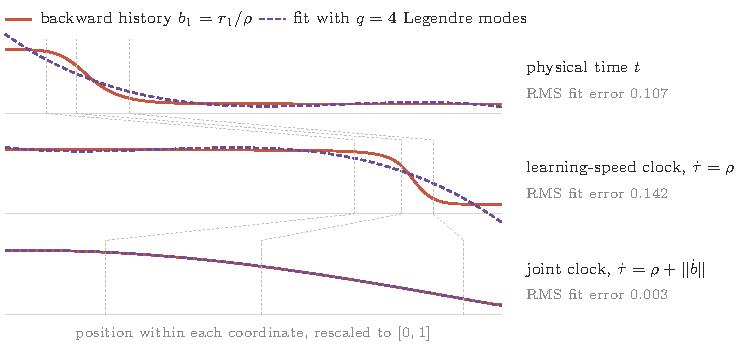
\includegraphics[width=0.92\textwidth]{figures/clocks.pdf}
 \caption{\textbf{Why the clock matters, on a toy signal.}  Two residuals
 decay at different rates, $r_1=e^{-4t}$ and $r_2=0.05\,e^{-t/2}$, so the
 normalized backward signal $b=r/\rho$ switches direction late, when the loss
 is already small.  Its first component is drawn in physical time, in the
 learning-speed clock and in the joint clock, each rescaled to $[0,1]$, with a
 least-squares fit by four Legendre modes; dotted lines join the same physical
 instants.  The learning-speed clock compresses the late phase and sharpens the
 switch; the joint clock spreads it out.  The three fit errors are measured in
 three different coordinates, so they illustrate how smooth the history is in
 each, not a common-metric comparison of closure errors; the joint closure
 itself uses the residual-weighted projection with a Gram matrix.}
 \label{fig:clock}
\end{figure}

\paragraph{Construction.}
Let $\Psi$ be the concatenation over $\ell\ge2$ and $a$ of the forward and
residual-weighted backward responses $(h^{(\ell-1)}_a,b^{(\ell)}_a)$, so that the
clock \eqref{eq:new-clock} reads $\dot\tau=g=\rho+\norm{\dot\Psi}_2$ and
$\norm{\dd\Psi/\dd\tau}\le1$.  History is placed at $\xi=\tau(s)$ with mass
$\rho(s)\dd s$, while the prefix $[0,1]$ carries Lebesgue mass and constant
initial responses; the resulting measure $\mu_t$ satisfies $\dd\mu_t\le\dd\xi$.
With $p=(p_0,\ldots,p_{q-1})^\top$ evaluated at $\xi/\tau$, $e=(1,\ldots,1)^\top$,
and the triangular matrix $\mathsf T_{kk}=k$, $\mathsf T_{kj}=2j+1$ for $j<k$
(zero above the diagonal), the state consists of the moment matrices
$\bar h^{(\ell-1)}_a=\int h^{(\ell-1)}_a(\xi)\,p^\top\dd\mu_t$,
$\bar\delta^{(\ell)}_a=\int b^{(\ell)}_a(\xi)\,p^\top\dd\mu_t$ and one shared
Gram matrix $G=\int pp^\top\dd\mu_t$, which evolve by
\begin{align}
 \widehat W^{(\ell)}&=W_0^{(\ell)}-\frac{2}{nm}\sum_a
 \bigl(\bar\delta^{(\ell)}_aG^{-1}(\bar h^{(\ell-1)}_a)^\top
 -b^{(\ell)}_a(0)\,h^{(\ell-1)}_a(0)^\top\bigr),\nonumber\\
 \dot{\bar h}^{(\ell-1)}_a&=\rho\,h^{(\ell-1)}_ae^\top-(g/\tau)\,\bar h^{(\ell-1)}_a\mathsf T^\top,
 \qquad
 \dot{\bar\delta}^{(\ell)}_a=r_a\delta_a^{(\ell)}e^\top-(g/\tau)\,\bar\delta^{(\ell)}_a\mathsf T^\top,
 \nonumber\\
 \dot G&=\rho\,ee^\top-(g/\tau)(\mathsf TG+G\mathsf T^\top),     \label{eq:new-ode}
\end{align}
with $G(0)=\diag(1,\tfrac13,\ldots,\tfrac1{2q-1})$, only the zeroth moment
columns nonzero initially, and the prefix product subtracted so that
$\widehat W^{(\ell)}(0)=W_0^{(\ell)}$.  With $h^{(\ell-1)*}_a=\bar h^{(\ell-1)}_aG^{-1}e$
and $b^{(\ell)*}_a=\bar\delta^{(\ell)}_aG^{-1}e$, differentiating the
reconstruction cancels every $g/\tau$ term and gives the defect
$E_\ell=\frac{2\rho}{nm}\sum_a(b^{(\ell)}_a-b^{(\ell)*}_a)(h^{(\ell-1)}_a-h^{(\ell-1)*}_a)^\top$,
of the same product form as \eqref{eq:defect}.

\paragraph{Step 1: a lower bound on the dense residual.}
Assume $\rho_0>0$ as stated, and use the compact physical ball $\mathcal B$ from
\Cref{app:proof-old}.  Retain the constants
$\alpha_\ell,\beta_\ell,\varrho,S,\mathsf A,V,\Lambda_F$ from the proof of \Cref{thm:old}.  On
this ball the output map has a finite Lipschitz constant $c_f$: prediction and
residual RMS change by at most $c_f\norm{\theta-\theta'}$.  Along dense flow,
\[
 |\dot\rho_{\rm dense}|\le c_f\norm{F(\theta)}
 \le c_fV\rho_{\rm dense}.
\]
Consequently
\begin{equation}
 \rho_{\rm dense}(t)\ge
 \mu:=\rho_0e^{-c_fVT}>0,\qquad 0\le t\le T.          \label{eq:dense-rho-lower}
\end{equation}

\paragraph{Step 2: an exact weighted projection energy.}
Consider the maximal regular closure interval stopped before either its
physical state leaves $\mathcal B$ or its residual reaches $\mu/2$.  We first
derive a clock bound on this stopped interval without assuming small projection
error.  For any inserted vector history $f$, let
\[
 D_f=\norm{f-\Pi_t f}_{L^2(\mu_t)}^2
 =\int\norm f^2\dd\mu_t-\operatorname{tr}(B_fG^{-1}B_f^\top).
\]
Differentiating $G^{-1}G=I$ gives
\[
 \frac{\dd}{\dd t}G^{-1}
 =-\rho G^{-1}ee^\top G^{-1}
 +(g/\tau)(G^{-1}\mathsf T+\mathsf T^\top G^{-1}).
\]
Together with \eqref{eq:new-ode}, this cancels every dilation term and yields
\begin{equation}
 \dot D_f=\rho\norm{f-f^*}^2,\qquad
 D_f(t)=\int_0^t\rho\norm{f-f^*}^2\dd s.             \label{eq:new-energy}
\end{equation}
The initial error is zero because every prefix is constant.  Thus
\eqref{eq:defect-energy} holds with the weighted errors in
\eqref{eq:new-energy}.

\paragraph{Step 3: order-independent coarse bounds.}
Put
\[
 Q=m\sum_{\ell=2}^L(\alpha_{\ell-1}^2+\beta_\ell^2),
 \qquad C_0=\frac{\mathsf A Q}{nm}.
\]
The total mass of $\mu_t$ is at most $\mathsf A=1+S$.  Projection error is no
larger than raw history energy, including the matching prefixes.  Applying
$2\sqrt{uv}\le u+v$ in the defect estimate gives the order-independent bounds
\begin{equation}
 \int_0^t\norm E\dd s\le C_0,\qquad
 \int_0^t\norm{\dot{\widehat\theta}}\dd s
 \le VS+C_0.                                         \label{eq:coarse-new}
\end{equation}
The second inequality uses $\dot{\widehat\theta}=F(\widehat\theta)+E$ and
$\int_0^t\norm F\dd s\le V\int_0^t\rho\dd s\le VS$.  This total-variation
estimate is stronger than bounded physical position, and it is obtained before
any clock bound.

\paragraph{Step 4: a clock bound without a cap.}
It remains to control the derivative of the normalized response map.  Let
$\tilde r=r/\rho\in\R^m$.  Then
\begin{equation}
 \norm{\tilde r}^2=m,\qquad
 D\tilde r[v]=
 \left(I-\frac{\tilde r\tilde r^\top}{m}\right)\frac{Dr[v]}{\rho}. \label{eq:normalized-residual-derivative}
\end{equation}
The matrix in parentheses is an orthogonal projector, and $\rho\ge\mu/2$ on the
stopped interval.  Differentiating the forward and backward recurrences uses
only bounded physical weights and bounded first two activation derivatives on
compact preactivation intervals; the first layer uses only $\phi'$.  Hence
there is a finite, $q$-independent constant $J$ such that
\[
 \norm{D\Psi(\vartheta)}_{\rm op}\le J
\]
throughout the stopped tube.  The stated local smoothness also makes this
derivative locally Lipschitz.  Since
$\dot\Psi=D\Psi(\widehat\theta)\dot{\widehat\theta}$, \eqref{eq:coarse-new}
now gives
\begin{equation}
 \tau_q(t)=1+\int_0^t(\rho+\norm{\dot\Psi})\dd s
 \le\mathsf A+J(VS+C_0)=:\Lambda_T.                 \label{eq:new-clock-bound}
\end{equation}
No clock cap has been assumed or inserted.

\paragraph{Step 5: the sharp joint approximation estimate.}
We can now use the sharper approximation estimate.  The entire concatenated
history $\overline\Psi(\xi)$ is constant on the prefix, continuous at its join
and, on the physical history,
\[
 \norm{\partial_\xi\overline\Psi}
 =\frac{\norm{\dot\Psi}}{\rho+\norm{\dot\Psi}}\le1.
\]
Therefore $\int_0^{\tau_q}\norm{\overline\Psi'}^2\dd\xi\le \tau_q-1$.  The weighted
projection is a best approximation in $L^2(\mu_t)$, and $\dd\mu_t\le\dd\xi$, so
comparison with the ordinary Legendre projection and \Cref{lem:legendre} give
the joint bound
\begin{equation}
 \sum_{\ell,a}(D_{h,\ell,a}+D_{b,\ell,a})
 \le\frac{\tau_q^2(\tau_q-1)}{4q(q+1)}
 \le\frac{\Lambda_T^2(\Lambda_T-1)}{4q(q+1)}.       \label{eq:new-joint-tail}
\end{equation}
This is one estimate for the concatenated path; it does not introduce a
separate dimension factor per unit or layer.

\paragraph{Step 6: feedback and continuation.}
Combining \eqref{eq:defect-energy}, \eqref{eq:new-clock-bound},
\eqref{eq:new-joint-tail} and $2\sqrt{uv}\le u+v$ yields
\begin{equation}
 \int_0^t\norm E\dd s
 \le\frac{\Gamma_{\mathrm{JF}}}{q(q+1)},\qquad
 \Gamma_{\mathrm{JF}}=\frac{\Lambda_T^2(\Lambda_T-1)}{4nm}.     \label{eq:new-sharp-defect}
\end{equation}
Subtracting the dense flow and applying the Lipschitz constant $\Lambda_F$ and Gronwall's
inequality gives
\begin{equation}
 \norm{\widehat\theta_q(t)-\theta(t)}
 \le\frac{\Gamma_{\mathrm{JF}}e^{\Lambda_FT}}{q(q+1)}.                  \label{eq:new-feedback}
\end{equation}

Choose $q_0(T)$ so that, for every $q\ge q_0(T)$,
\begin{equation}
 \frac{\Gamma_{\mathrm{JF}}e^{\Lambda_FT}}{q(q+1)}\le\frac12,\qquad
 c_f\frac{\Gamma_{\mathrm{JF}}e^{\Lambda_FT}}{q(q+1)}\le\frac\mu4.      \label{eq:new-order-condition}
\end{equation}
The first inequality rules out physical exit, because the dense path stays at
distance one from $\partial\mathcal B$.  The second, together with
\eqref{eq:dense-rho-lower}, gives $\widehat\rho\ge3\mu/4>\mu/2$, ruling out
residual exit.

Finally, the matching prefix supplies, at every fixed $q$,
\begin{equation}
 G(t)\succeq\int_0^1p(\xi/\tau_q(t))p(\xi/\tau_q(t))^\top\dd\xi. \label{eq:prefix-gram}
\end{equation}
The right side is positive definite, since a zero quadratic form would make a
nonzero polynomial vanish on an interval.  Its entries vary continuously with
$\tau_q$, so on $1\le \tau_q\le\Lambda_T$ its least eigenvalue has a positive minimum
$\gamma_{q,T}$; this minimum need not be uniform in $q$.  The moment integral
representations, finite history mass, bounded responses and bounded
fixed-order polynomials then bound every raw coordinate.  Together with the
physical, residual, clock and Gram bounds, the full state lies in a compact
subset of its locally Lipschitz domain.  A finite maximal endpoint therefore
extends, which proves continuation through $T$ and completes the theorem,
with implied constant $\Gamma_{\mathrm{JF}}e^{\Lambda_FT}$. \qed

\subsection*{Implementation of the joint clock}
\label{app:joint-impl}

Equation \eqref{eq:new-clock} appears implicit only because $\dot\Psi$ is
written compactly; no nonlinear solve for $g$ is needed.  The internal
velocities do not depend on $g$, so they can be computed first.  Begin with
$G^{-1}e$, the endpoint fits $h^*,b^*$, and the internal velocities
\begin{equation}
 V_\ell=\dot{\widehat W}^{(\ell)}=-\frac{2\rho}{nm}\sum_a
 \left[b^{(\ell)}_a(h^{(\ell-1)*}_a)^\top+
 b^{(\ell)*}_a(h^{(\ell-1)}_a-h^{(\ell-1)*}_a)^\top\right]. \label{eq:internal-velocity}
\end{equation}
These expressions contain no $g$.  Next compute $V_1=F_1$ and $V_w=F_w$, and run
a directional forward pass,
\[
 \dot z_a^{(1)}=V_1x_a/\sqrt d,\qquad
 \dot z_a^{(\ell)}=V_\ell h_a^{(\ell-1)}+
 \widehat W^{(\ell)}\dot h_a^{(\ell-1)},\qquad
 \dot h_a^{(\ell)}=\phi'(z_a^{(\ell)})\od\dot z_a^{(\ell)},
\]
which gives $\dot r$ and $\dot\rho$.  A reverse directional pass then
differentiates the backward recurrence, using $\phi''$ for $\ell\ge2$, and
yields
\[
 \dot b^{(\ell)}_a=\frac{\dot r_a\delta_a^{(\ell)}+
 r_a\dot\delta_a^{(\ell)}}{\rho}-b^{(\ell)}_a\frac{\dot\rho}{\rho}.
\]
Only then do we evaluate $g=\rho+\norm{\dot\Psi}$ and, finally,
\eqref{eq:new-ode}.  Matrix and transpose actions use the same reconstructed
operator.  In practice one factors $G$ and solves linear systems; an explicit
inverse is unnecessary.

The joint clock is more regular in approximation coordinates, but it is not
automatically better at low order.  At $q=1$ the polynomial space consists of
constants, so changing the coordinate alone leaves the physical constant-mode
closure unchanged.  Higher orders pay for Gram solves and derivative passes,
and the theoretical constants can be large.

\section{Exact compression in a deep linear benchmark}
\label{app:exact}

Take one datum $x=1$, a label $y$, three linear hidden layers with order-one
initialization, mobilities $(n\kappa,\kappa,\kappa,n\kappa)$, and the normalized
factors $u=W^{(1)}/\sqrt n$, $v=W^{(4)}/\sqrt n$, so that
$f_n=v^\top W^{(3)}W^{(2)}u$.  Packing the four factors into the cyclic block
matrix $\mathcal C_n$ with blocks $v^\top,u,W^{(2)},W^{(3)}$ below and above the
diagonal gives $f_n=\tfrac14\operatorname{Tr}\mathcal C_n^4$, and the feature
derivative of $\mathcal C_n$ is $(\mathcal C_n^\top)^3$.

\begin{theorem}[Exact operator closure]
\label{thm:operator}
There are a separable Hilbert space, a bounded initialized source $\mathcal C_0$
and a unique global trace-class increment $Q(t)$ with
\[
 \mathcal C=\mathcal C_0+Q,\qquad f=\tfrac14\operatorname{Tr}\mathcal C^4,\qquad
 \dot Q=-2\kappa(f-y)(\mathcal C_0^*+Q^*)^3,\qquad Q(0)=0 .
\]
The kernel is $K=\operatorname{Tr}[\mathcal C^3(\mathcal C^*)^3]$, the residual
obeys $\dot r=-2\kappa rK$, and $\norm{Q(t)}_1\le2|y|\sqrt{\kappa t}$.  For every
fixed $T$, finite gradient flow, and gradient descent for every step sequence
tending to zero, converge in probability to $(f,K,\cL)$ uniformly on $[0,T]$.
\end{theorem}

The proof builds $\mathcal C_0$ as the limit of initialized word statistics on a
colored Fock space, obtains global existence from trace-norm control, passes to
the width limit through finite-word Picard iterates, and treats gradient descent
as an exact Euler step for $Q$.

\begin{theorem}[Restricted scalar nonclosure]
\label{thm:nonclosure}
In the same model, no encoder formed from a fixed finite list of complete tensor
contractions of $(u,W^{(2)},W^{(3)},v)$ with connected-graph degree bounded
independently of width admits a width-independent polynomial autonomous ODE (or
finite-order local polynomial PDE) and a polynomial output readout reproducing
the output dynamics on a nonempty open set of states for all sufficiently large
widths.
\end{theorem}

The $(2j-1)$st feature derivative of the output contains the connected
contraction
\[
 u^\top\bigl((W^{(2)})^\top(W^{(3)})^\top W^{(3)}W^{(2)}\bigr)^ju
\]
of degree $4j+2$.  Polynomial operations on a bounded-degree alphabet form only
disjoint unions of connected components already present, and nonisomorphic
contraction graphs are linearly independent at large width, so this term cannot
be synthesized.  The theorem does not exclude arbitrary encoders, unrestricted
fields, or closures tailored to a single initialized trajectory.

\section{Accuracy and resource comparisons: derivations}
\label{app:comparison}
\label{app:size}

All comparisons concern the same dense population predictor $f_\infty$,
with the canonical mobility, data, Gaussian initialization and exactly zero
readout of \Cref{thm:alltime}.  Matching initial predictions alone would
not ensure this agreement.  Moving state means persistent updated scalars;
fixed initialized matrices, coefficient evaluators and temporary workspace
are accounted for separately.  Constants may depend on the fixed task,
including $m,d,L$, the Gram margin, activation bounds and test law.

\begin{definition}[Size at accuracy]
\label{def:size}
For a specified representation and a stated sufficient error certificate,
its size at accuracy $\varepsilon$ is the least moving state obtained by
choosing the representation's resolution parameters to satisfy that
certificate, at the specified horizon and confidence level.  This is a
sufficient representation cost, not an algorithmic lower bound.
\end{definition}

\subsection{The all-time certificate and its quantitative limits}
\label{app:comparison-opt}

For $0<T\le\infty$, use the finite-horizon restriction of
\eqref{eq:test-metric},
\begin{equation}
 E_\mu(g,f;T)=\left[\int\sup_{0\le t\le T}
                  |g(t,x)-f(t,x)|^2\,\mu(\dd x)\right]^{1/2}.
 \label{cmp:test-error}
\end{equation}
The test law has finite second input moment.  This whole-input metric
controls the difference of test RMSEs against any target in $L^2(\mu)$,
uniformly in time; it does not assert that $f_\infty$ generalizes well.
We use $T=\infty$ for the response-memory theorem.  Finite-$T$ certificates
for other methods below remain finite-$T$ comparisons unless an additional
tail estimate extends them to this same all-time metric.

Let $D_n=E_\mu(f_n,f_\infty;\infty)$.  Prediction transfer from the
normalized distance \eqref{eq:normalized-distance}, followed by the
triangle inequality, gives on the common initialization events
\begin{equation}
 E_\mu(\widehat f_{n,q},f_\infty;\infty)
 \le C_\mu\omega(q)+B_{n,\mu}+D_n,
 \qquad
 \omega(q)=q^{-2}\exp\!\left\{K\sqrt{\log(e+q)}\right\}.
 \label{cmp:triangle}
\end{equation}
Here $B_{n,\mu}$ is the closure's dense-carrier transfer remainder after
prediction transfer.  Both $B_{n,\mu}$ and $D_n$ tend to zero in probability;
the theorem supplies no numerical width rate for either.  Their sum is the
order-independent remainder $b_{n,\mu}$ in \Cref{thm:alltime}.
The events and remainders are common to all $q$, so every deterministic
$q_n\to\infty$ gives convergence in the all-time metric without an
interchange of fixed-order limits.

The moving-state counts are
\begin{equation}
 M_{\rm dense}(n)=(L-1)n^2+n(d+1),\qquad
 M_{\rm mem}(n,q)=2(L-1)mnq+n(d+1)+O(1).
 \label{cmp:moving-counts}
\end{equation}
For fixed positive integers $m,d$ and fixed $L\ge2$,
$q_n\to\infty$ and $q_n=o(n)$ imply
$M_{\rm mem}/M_{\rm dense}\to0$, proving \Cref{cor:compression}.
For example, $q_n=\lceil\log\log(e^e+n)\rceil$ already suffices.
This is a convergence and compression statement along the same width
sequence, not a comparison of the narrowest networks attaining a tolerance.

\paragraph{Conditional costs at a fixed confidence.}
An additional quantitative benchmark is
\begin{equation}
 D_n=O_{\Pr}(n^{-1/2}),\qquad
 B_{n,\mu}=O_{\Pr}(n^{-1/2}).
 \label{cmp:root-width-hypotheses}
\end{equation}
The second hypothesis does not follow from the first: controlling dense
predictions need not quantify the empirical transfer of dense backward
carriers.  Neither follows merely from a fixed-program population limit or
the perturbative fluctuation calculation of \citet{bordelon2023finite}.
These hypotheses are needed in the same all-time metric and probability
convention.  In particular, convergence in probability in
\Cref{thm:alltime} is not an unconditional RMS rate.

Under \eqref{cmp:root-width-hypotheses}, at any fixed confidence one may take
$n=O(\varepsilon^{-2})$ with a sufficiently large constant and choose $q$
so that $C_\mu\omega(q)\le\varepsilon/2$.  Writing $z=\log q$ gives
$\log\omega(q)=-2z+K\sqrt z+o(1)$, hence a sufficient order satisfies
\begin{equation}
 \log q=\tfrac12\log(1/\varepsilon)
                  +O\!\left(\sqrt{\log(1/\varepsilon)}\right),\qquad
 q=\varepsilon^{-1/2+o(1)}.
 \label{cmp:near-quadratic-order}
\end{equation}
The constant in the $O(\sqrt{\log(1/\varepsilon)})$ correction is chosen
sufficiently large to enforce the error inequality.
Consequently, for fixed $m,d,L$,
\begin{equation}
 M_{\rm mem}=O\!\left(\varepsilon^{-5/2+o(1)}\right),\qquad
 M_{\rm dense}=O(\varepsilon^{-4}).
 \label{cmp:conditional-cost}
\end{equation}
These are sufficient costs from the two certificates; no optimality or
lower bound is asserted.  Without \eqref{cmp:root-width-hypotheses},
\Cref{cor:compression} still holds, but \eqref{cmp:conditional-cost} is
not a proved accuracy-cost law.

For reference, a pure-power certificate
$A n^{-1/2}+Bq^{-p}\le\varepsilon$, $p>0$, leads to the continuous
allocation problem $\min u^{-2}(\varepsilon-u)^{-1/p}$, where
$u=A/\sqrt n$.  Its logarithmic derivative is
$-2/u+1/[p(\varepsilon-u)]$, with positive derivative, and its objective
diverges at both endpoints.  Thus
\begin{equation}
 u_*=\frac{2p\varepsilon}{2p+1},\qquad
 n_*=\frac{(2p+1)^2A^2}{4p^2\varepsilon^2},\qquad
 q_* =\left(\frac{(2p+1)B}{\varepsilon}\right)^{1/p}.
 \label{cmp:allocation}
\end{equation}
Upward rounding preserves feasibility.  The near-quadratic theorem has a
subpower correction and an unquantified width remainder, so the exact
$p=2$ allocation is not its unconditional optimum.

The original residual-speed implementation permits full-batch arithmetic
per right-hand-side evaluation
\begin{equation}
 C_{\rm dense}=O(Lmn^2+mnd),\qquad
 C_{\rm mem}=O(Lmn^2+Lm^2nq+Lmnq+mnd).
 \label{cmp:response-work}
\end{equation}
The terms account for initialized matrix actions, learned-factor actions,
moment updates and first-layer work.  The closure also retains
$(L-1)n^2$ initialized hidden entries as fixed data; activation workspace
is $O(Lmn)$.
The theorem therefore compresses evolving state, without an automatic
improvement of total storage or arithmetic at a prescribed accuracy.

\subsection{A matched tangent hierarchy}
\label{app:comparison-nth}

For sufficiently differentiable activations, the canonical mobility
$\mathcal D_n=\diag(nI,I,\ldots,I,nI)$ defines
\begin{align*}
 K^{(2)}(x,z)&=\nabla_\theta f(x)^\top\mathcal D_n\nabla_\theta f(z),\\
 K^{(j+1)}(x_1,\ldots,x_{j+1})&=
 (\nabla_\theta K^{(j)}(x_1,\ldots,x_j))^\top
 \mathcal D_n\nabla_\theta f(x_{j+1}).
\end{align*}
The chain rule gives the exact matched hierarchy
\begin{equation}
 \dot f(x)=-\frac{2}{m}\sum_a r_aK^{(2)}(x,x_a),\qquad
 \dot K^{(j)}=-\frac{2}{m}\sum_a r_aK^{(j+1)}(\ldots,x_a).
 \label{cmp:nth-flow}
\end{equation}
Truncation through order $q\ge2$ retains exact initial coefficients and
freezes $K^{(q)}$.  A population implementation additionally needs limiting
initial coefficients and a valid limiting hierarchy for this mobility.
The $C^{1,1}$ activation class of \Cref{thm:alltime} alone does not supply
the higher derivatives needed to define arbitrary orders.

\paragraph{A conditional finite-time certificate.}
Suppose on $[0,T]$ that $|K^{(j)}|\le B_j$ when the first argument ranges
over the training inputs and a controlled test set, and all other arguments
are training inputs.  Set $R=1+\sup_{t,a}|r_a(t)|$ and stop the truncated
flow at predictor error one.  Its residuals are then bounded by $R$.
For the corresponding supremum predictor and kernel errors,
\begin{align}
 e_q(t)&\le2RB_{q+1}t,\nonumber\\
 e_j(t)&\le\int_0^t(2Re_{j+1}+2B_{j+1}e_f)\dd s
                  \quad(2\le j<q),\nonumber\\
 e_f(t)&\le\int_0^t(2Re_2+2B_2e_f)\dd s.
 \label{cmp:nth-recursion}
\end{align}
Successive substitution integrates the top forcing $q$ times.  The feedback
kernels are
\[
 2B_{k+2}\frac{(2R(t-s))^k}{k!},\qquad 0\le k\le q-2.
\]
Bounding these at $T$ and applying Gronwall yields
\begin{equation}
 \sup_{t\le T}e_f(t)\le
 B_{q+1}\frac{(2RT)^q}{q!}\exp(\Lambda_{q,T}T),\qquad
 \Lambda_{q,T}=2\sum_{k=0}^{q-2}B_{k+2}\frac{(2RT)^k}{k!}.
 \label{cmp:nth-bound}
\end{equation}
If this bound is below one, it rules out first exit, while the triangular
integral equations bound all training tensors and ensure continuation.
It controls \eqref{cmp:test-error} for a test law supported on the controlled
set; an unbounded test law needs an integrable envelope.  Random coefficients
and their approximation errors need the same probability convention as the
compared predictor.

For example, the additional factorial-growth and stability conditions
$B_j\le UV^{j-2}(j-2)!$ and $\chi=2RVT<1$ give
$\Lambda_{q,T}\le2U/(1-\chi)$ and error at most $D\chi^q/q$, where
$D=(U/V)\exp\{2UT/(1-\chi)\}$.  For this certificate, with
$\lambda_\chi=\log(1/\chi)$,
\begin{equation}
 q_\varepsilon=\max\left\{2,\left\lceil
 \frac{W(\lambda_\chi D/\varepsilon)}{\lambda_\chi}
 \right\rceil\right\},\qquad
 M_{\rm NTH}=\sum_{j=1}^{q_\varepsilon-1}m^j
 =\frac{m^{q_\varepsilon}-m}{m-1}\quad(m\ge2).
 \label{cmp:nth-memory}
\end{equation}
Here $W(z)e^{W(z)}=z$.  The fixed top tensor and direct work each have
order $m^{q_\varepsilon}$.  At fixed $m\ge2$ and $\chi$ the moving count
is of order
$[D/(\varepsilon\log(D/\varepsilon))]^{\log m/\lambda_\chi}$.
The exponent depends on a certified $\chi$; a universal $\log_2m$ exponent
does not follow.  Analyticity of $\tanh$ by itself does not establish these
bounds, and $\chi\ge1$ makes this particular certificate inconclusive.
Population use needs resource-independent constants and access to the
initial mixed test-input kernels.  No all-time conclusion follows from
this finite-$T$ argument.

\paragraph{What the published NTH theorem supplies.}
In their native NTK parameterization,
\citet[Theorem~2.6]{huang2020nth} prove, after exchanging width/sample symbols,
\begin{align}
 \frac{\norm{f(t)-\widetilde f(t)}_2}{\sqrt m}
 &\lesssim\frac{(1+t)t^{q-1}}{n^{q/2}}\min\{t,m/\lambda\},\nonumber\\
 t&\le\min\left\{\frac{c\sqrt{\lambda n/m}}{(\log n)^C},
 \frac{n^{q/[2(q+1)]}}{(\log n)^{C'}}\right\}.
 \label{cmp:published-nth}
\end{align}
This assumes their initialization, even $q$, bounded activation derivatives
through $2q+1$, bounded nondegenerate inputs with uniformly independent
subsets through size $2q+1$, and an initial kernel eigenvalue gap.
Loss normalization only rescales time by a constant.  The estimate concerns
training RMS in that parameterization; it supplies neither a whole-input
all-time bound for the canonical feature-learning target nor the factorial
and stability hypotheses above.

For whole-function queries the matched hierarchy has a finite coefficient
representation.  Set $u_a=-2\widetilde r_a/m$, $I_\varnothing=1$ and
$\dot I_{a_1\cdots a_k}=u_{a_1}I_{a_2\cdots a_k}$, with zero initial
values for nonempty words.  Repeated integration gives
\begin{equation}
 \widetilde f_q(t,x)=f_0(x)+\sum_{k=1}^{q-1}\sum_{a_1,\ldots,a_k}
 K_0^{(k+1)}(x,x_{a_1},\ldots,x_{a_k})I_{a_1\cdots a_k}(t).
 \label{cmp:signature}
\end{equation}
The moving count agrees with \eqref{cmp:nth-memory}; query work additionally
includes the fixed mixed-kernel evaluators.  For $m=1$, all coefficients
are $I_k=s^k/k!$ with $\dot s=u$, so one moving scalar suffices.  Thus the
direct tensor count is a representation cost, not a universal lower bound.

\subsection{A specified streamed DMFT solver and stored histories}
\label{app:comparison-dmft}

The self-consistency solver of
\citet[Appendix~B, Algorithm~1]{bordelon2022dmft} stores covariance and
response kernels indexed by input and time pairs.  Matching scales requires
$\gamma=\sqrt n$, internal coordinates $U^{(\ell)}=\sqrt nW^{(\ell)}$,
and the same readout law and loss normalization.  A fixed-program Tensor
Programs limit \citep[Algorithm~1, Theorem~7.4]{yang2021tensor} does not
itself prescribe a convergent numerical solver or quantify its error.

For $N_t$ time steps, $S$ sampled paths and $I$ self-consistency sweeps,
factoring a dense covariance costs $O((mN_t)^3)$ per layer.  Streaming one
path and its full response Jacobian while accumulating kernel averages gives
the implementable upper bounds
\begin{equation}
 M_{\rm D}=O(Lm^2N_t^2),\qquad
 C_{\rm D,total}=O(IL(S+1)m^3N_t^3),\qquad
 C_{\rm D,step}=O(IL(S+1)m^3N_t^2).
 \label{cmp:dmft-cost}
\end{equation}
Memory includes kernel and Jacobian workspace; the last cost is amortized.
Mixed kernels and test paths must also be available for test prediction.
These are costs for this solver, not lower bounds for TP or DMFT.

A sufficient stability certificate would be a discrete self-consistency map
$\mathcal F$ that is a $\kappa$-contraction, $\kappa<1$, in a norm
controlling test outputs.  If its sampled approximation differs uniformly
by $\zeta$ and a computed point has residual at most $\eta_0$, then
\[
 \norm{\widehat z-z_*}\le\eta_0+\zeta+
       \kappa\norm{\widehat z-z_*}
 \quad\Longrightarrow\quad
 \norm{\widehat z-z_*}\le\frac{\eta_0+\zeta}{1-\kappa}.
\]
With a Lipschitz output map, uniform sampling control and a stable
order-$\sigma$ time discretization, this would yield, at the specified
confidence and finite horizon,
\begin{equation}
 E_\mu(g_{S,N_t},f_\infty;T)
 \le A_{\rm D}S^{-1/2}+B_{\rm D}(T/N_t)^\sigma+\eta.
 \label{cmp:dmft-error}
\end{equation}
The constants include stability amplification.  Grid-uniform Monte Carlo
control, a certified numerical order, self-consistency stability and
whole-input output control are additional hypotheses, not consequences of
the cited limiting descriptions.  An all-time comparison further requires
a certified treatment of the remaining time tail.

Conditionally on \eqref{cmp:dmft-error} for a fixed $\sigma$, assigning fixed
fractions of $\varepsilon$ to the three terms gives
$S=O(\varepsilon^{-2})$, $N_t=O(T\varepsilon^{-1/\sigma})$ and
$M_{\rm D}=O(Lm^2T^2\varepsilon^{-2/\sigma})$.
Streaming moves the sampling cost into work; it does not eliminate it.
One cannot improve this exponent by declaring arbitrarily high numerical
order without the corresponding regularity, stability, constants and stage
costs.  There is no certified universal DMFT accuracy exponent here.

A separate finite-network baseline stores every Euler update:
\[
 W^{(\ell)}_k=W^{(\ell)}_0-\frac{2\Delta}{nm}
 \sum_{j<k,a}r_{a,j}\delta^{(\ell)}_{a,j}
                          (h^{(\ell-1)}_{a,j})^\top.
\]
Its moving memory is $O(LmnN_t)$, fixed memory $O(Ln^2)$ and late-step
work $O(Lmn^2+Lm^2nN_t)$.  A specified method with a fixed number of
stages has the same storage order.  If it also has a matched certificate
$A/\sqrt n+D_{\rm h}(T/N_t)^\sigma$, \eqref{cmp:allocation} gives
sufficient moving state
$O(LmA^2T D_{\rm h}^{1/\sigma}\varepsilon^{-(2+1/\sigma)})$.
This conditional finite-$T$ calculation stores finite-network updates;
it is distinct from sampling a population response system.  Its numerical
order and horizon dependence need their own certificates.

The resource formulas identify what each representation stores and which
additional estimates would make accuracy comparisons quantitative.  Only
\Cref{thm:alltime,cor:compression} supply the all-time response-memory
convergence claim used here; none of the conditional exponents establishes
a universal ordering or an optimal complexity theorem.


\clearpage
\section{Supplementary fitted functions on the sphere}
\label{app:sphere-endpoints}

Figure~\ref{fig:sphere-orders} adds a three-dimensional-input, four-hidden-layer
example.  The sphere RMS discrepancies from dense are $0.02193$, $0.01280$,
and $0.00454$ for $q=1,2,3$.  Dense and the three closures reach training
RMS $\leq0.01$ at times $60$, $75.5$, $63.25$, and $60$, respectively.
This is supplementary fitted-function evidence outside the smooth-activation
theorems: ReLU is nonsmooth, and the endpoints are individually fitted.
Rendering the saved predictions does not independently reproduce training.

\begin{figure}[!htbp]
  \centering
  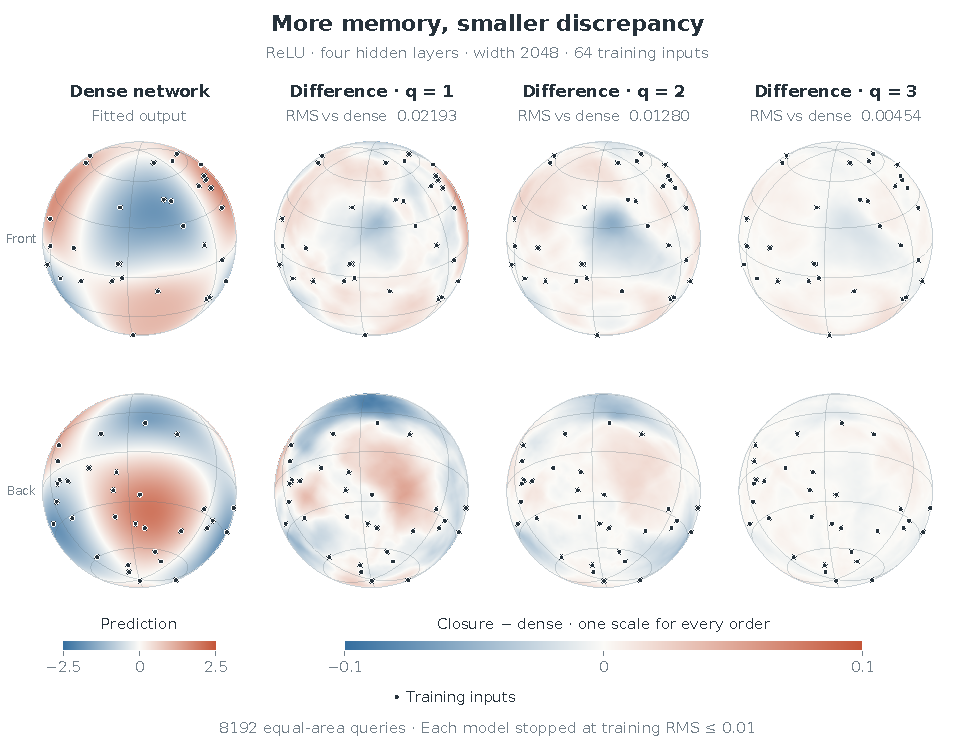
\includegraphics[width=\textwidth]{figures/sphere_orders.pdf}
  \caption{Saved fitted functions on the unit sphere for the target
  $\sqrt{105}\,x_1x_2x_3$, with four hidden ReLU layers of width $2048$ and
  $64$ training inputs.  The first column shows the dense output; the remaining
  columns show signed closure-minus-dense differences for $q=1,2,3$.
  Rows show complementary hemispheres, and black dots mark training inputs.
  Output colors use $[-2.5,2.5]$; every error panel uses $[-0.1,0.1]$.
  Surface colors interpolate saved queries on a triangular mesh; RMS values
  use the original $8192$ equal-area query values before interpolation.
  Models are compared at their individual training-RMS $\leq0.01$ endpoints,
  using one network seed and float32 Euler steps of $1/128$.
  The order trend is specific to this one-seed comparison.  These are
  fitted-function discrepancies, without a common-time trajectory comparison
  or a continuous-gradient-flow refinement certificate.}
  \label{fig:sphere-orders}
\end{figure}


\clearpage
\section{Supplementary two-hidden-layer circle gallery}
\label{app:circle-gallery}

\Cref{fig:shallow} shows the full two-hidden-layer task gallery, and
\Cref{tab:circle} collects the whole-circle RMS discrepancies of both depths
(the three-hidden-layer gallery is \Cref{fig:deep} in the main text).

\begin{table}[t]
\centering
\small
\caption{Whole-circle RMS difference between response memory and dense
training at individually fitted endpoints. Left: two hidden tanh layers,
width $2048$ (\Cref{fig:shallow}). Right: three hidden tanh layers,
width $4096$ (\Cref{fig:deep}).}
\label{tab:circle}
\begin{tabular}{lrrr@{\qquad}rrr}
\toprule
 & \multicolumn{3}{c}{two layers} & \multicolumn{3}{c}{three layers}\\
Task & $q=1$ & $q=3$ & $q=7$ & $q=1$ & $q=2$ & $q=3$\\
\midrule
Two outliers, alternating & 0.236 & 0.0730 & 0.00466 & 0.108 & 0.0238 & 0.0315\\
Quadrant, alternating & 0.341 & 0.0456 & 0.00155 & 0.275 & 0.0284 & 0.0585\\
Quadrant, paired & 0.0193 & 0.00282 & 0.00012 & 0.0122 & 0.00371 & 0.00121\\
Quadrant, center/edges & 0.0456 & 0.00488 & 0.00131 & 0.0790 & 0.0257 & 0.00725\\
Equally spaced, mixed & 0.0124 & 0.00053 & $4\times10^{-6}$ & 0.0150 & 0.00241 & 0.00028\\
\bottomrule
\end{tabular}
\end{table}

\begin{figure}[!htbp]
 \centering
 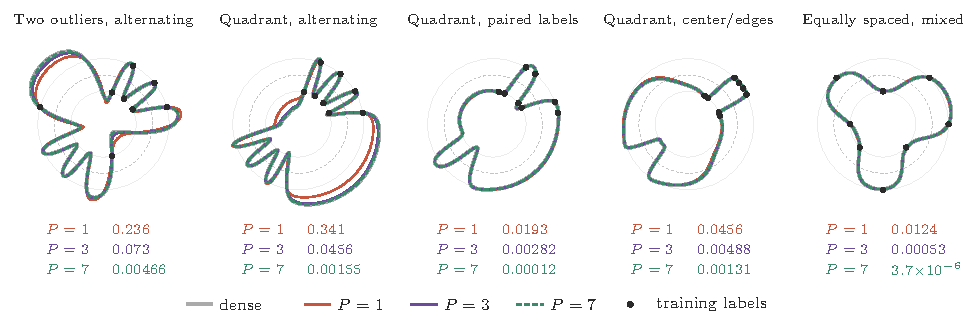
\includegraphics[width=\textwidth]{figures/circles_shallow.pdf}
 \caption{Fitted circle predictions for two hidden tanh layers, width $2048$,
 and response-memory orders $q=1,3,7$, using the dense references in
 \Cref{tab:circle}. Models are evaluated at their individual training-MSE
 $10^{-3}$ endpoints. Angle is input direction and radius is $3+f(\theta)$;
 rings, training labels and RMS values follow \Cref{fig:deep}. RMS is measured
 on $8192$ uniform circle points.}
 \label{fig:shallow}
\end{figure}

\section{Supplementary experimental figures}
\label{app:supp-figs}

\begin{figure}[!htbp]
 \centering
 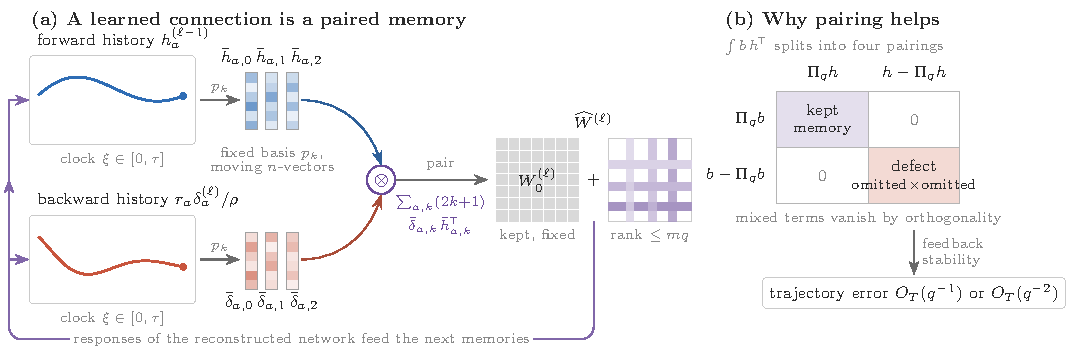
\includegraphics[width=\textwidth]{figures/mechanism.pdf}
 \caption{\textbf{A learned connection is a paired memory.}  (a)~For each
 hidden link and training sample, the forward response $h_a^{(\ell-1)}$ and the
 residual-weighted backward response $b_a=r_a\delta_a^{(\ell)}/\rho$ are
 recorded in the learning clock and projected onto the first $q$ shifted
 Legendre polynomials ($q=3$ shown).  The polynomial coordinates are fixed; the
 moment vectors $\bar h_{a,k},\bar\delta_{a,k}\in\R^n$ keep moving.  Pairing
 them gives a correction of rank at most $mq$, added to the fixed
 initialization $W_0^{(\ell)}$, and the responses of the reconstructed network
 feed the next memories.  (b)~Splitting each history into its projection
 $\Pi_q$ and remainder, the exact interaction $\int b\,h^\top$ is a sum of four
 pairings; the mixed ones vanish by orthogonality, so the memory misses only
 the product of the two omitted parts.}
 \label{fig:mechanism}
\end{figure}

\Cref{fig:mechanism} sketches the paired memory and the product form of its defect; \Cref{fig:moments} shows what Legendre moments retain of recorded response
histories; \Cref{fig:trajectory-rms} shows the RMS discrepancies behind
\Cref{fig:trajectory} at every shared time; \Cref{fig:order} shows the
three-hidden-layer order trends of \Cref{tab:circle} next to their numerical
sensitivity and the movement of the hidden features; \Cref{fig:mnist} shows
the MNIST predictions and residuals summarized in \Cref{sec:experiments}.

\begin{figure}[!htbp]
 \centering
 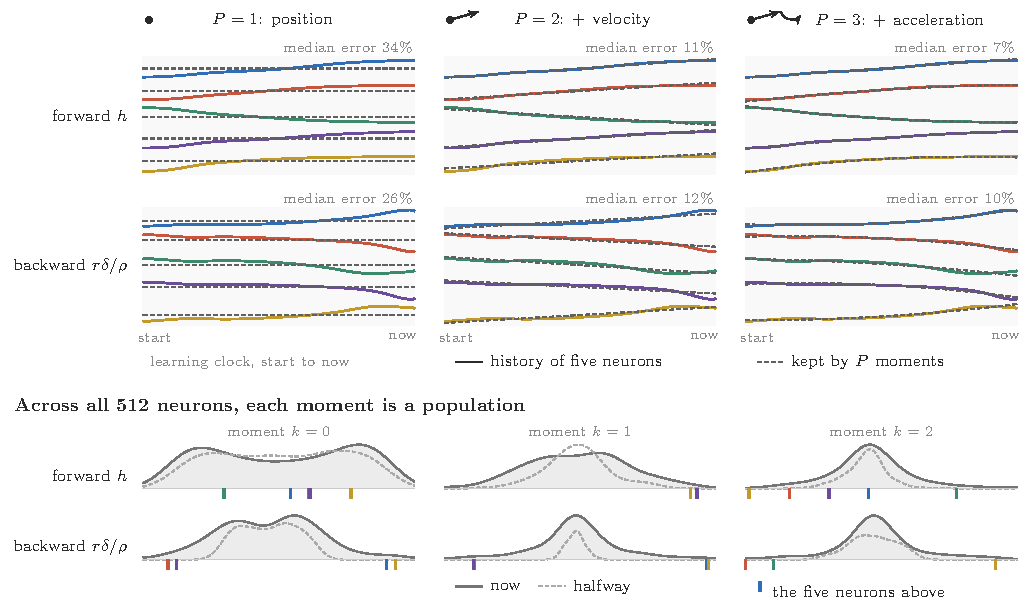
\includegraphics[width=\textwidth]{figures/moments.pdf}
 \caption{\textbf{What Legendre moments retain of a history.}  A network with
 two hidden tanh layers of width $512$ is trained by gradient descent on eight
 circle points, and the forward responses $h$ of one training input are
 recorded.  Top: three neurons over the whole of training in the
 learning-speed clock, with their projections onto $q=1,2,3$ Legendre modes
 (mean, linear trend, quadratic shape).  These are projections fitted
 afterwards to the recorded dense histories, not trajectories of the closure.
 Above each panel, the median over all $512$ neurons of the RMS projection
 error divided by the range of that neuron's history; for the backward
 histories $r\delta/\rho$ the same numbers are $26\%$, $12\%$ and $10\%$.
 Bottom: the plotted quantities are the normalized Legendre coefficients
 $(2k+1)\bar h_k/\tau$ of the fitted projection, not the stored moments
 $\bar h_k$; across neurons each coefficient is a population, shown for the
 history up to the midpoint of the learning clock and for the whole history,
 with the three neurons above marked.}
 \label{fig:moments}
\end{figure}

\begin{figure}[!htbp]
 \centering
 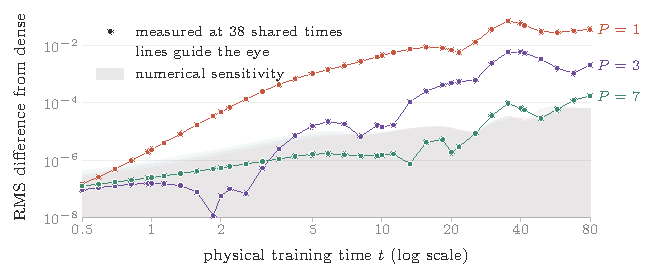
\includegraphics[width=0.8\textwidth]{figures/trajectory_rms.pdf}
 \caption{\textbf{Discrepancy from dense training at common physical times.}
 The paired-label task of \Cref{fig:trajectory}: RMS difference between
 response memory and the finer dense replay on $2048$ circle queries at the
 $38$ positive shared times, on a logarithmic time axis; the common
 initialization at $t=0$ is omitted.  Dots are measured; thin lines guide the
 eye.  Light shading extends from the axis floor to each order's coarse/fine
 sensitivity scale, obtained by summing the dense and closure prediction
 changes between the two integration tolerances; it is a numerical
 diagnostic, not a confidence interval or a certified error bound, and the
 smallest discrepancies of $q=3$ and $q=7$ lie at that scale.}
 \label{fig:trajectory-rms}
\end{figure}

\begin{figure}[!htbp]
 \centering
 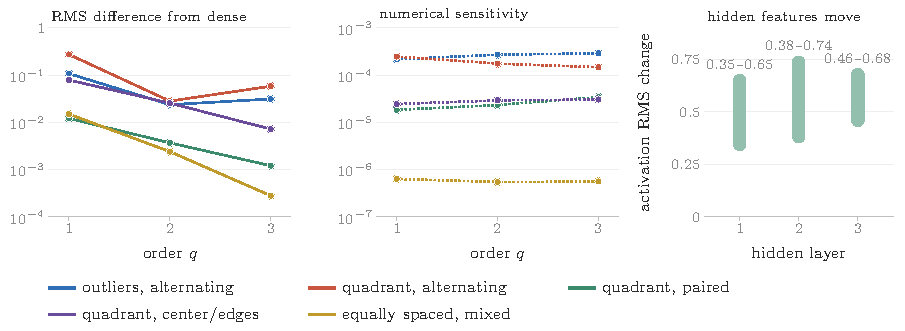
\includegraphics[width=\textwidth]{figures/orders.pdf}
 \caption{\textbf{Measured order trends and substantial feature movement.}
 Three-hidden-layer circle experiments, width $4096$, at individually fitted
 MSE $0.001$ endpoints. Left: discrepancies on $8192$ angles. Middle: sums of
 dense and closure coarse/fine prediction RMS changes, shown on a separate
 scale; these are numerical diagnostics, not confidence intervals or certified
 bounds. Right: ranges of absolute training-activation RMS changes from
 initialization across the 20 finest runs. Neither the endpoint comparisons
 nor the three tested orders establish a temporal tracking exponent.}
 \label{fig:order}
\end{figure}

\begin{figure}[!htbp]
 \centering
 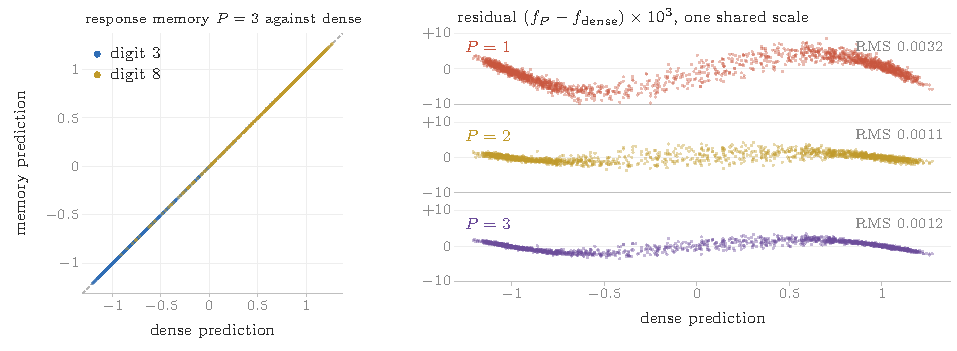
\includegraphics[width=\textwidth]{figures/mnist.pdf}
 \caption{\textbf{Agreement and its residual structure on MNIST.} Digits 3
 versus 8, 100 training images, two hidden tanh layers of width $4096$.
 Left: memory $q=3$ versus dense predictions on all $1984$ held-out images.
 Right: signed differences $f_q-f_{\mathrm{dense}}$, displayed in units of
 $10^{-3}$ with one vertical scale for all orders. RMS differences are
 $0.003248$, $0.001084$ and $0.001199$. Each model is evaluated at its own
 training-MSE $0.001$ endpoint. These are function discrepancies, not label RMSE.}
 \label{fig:mnist}
\end{figure}

\clearpage
\section{Frozen-kernel and same-rank controls}
\label{app:factors}

The frozen control uses the empirical tangent kernel of the same initialized
finite network, including the learning-rate metric. If $J_0(x)$ is its row
parameter Jacobian and $D$ has block mobilities $(n,1,n)$, then
$K_0(x,x')=J_0(x)D J_0(x')^\top$. For the training list $X$ and unhalved mean
squared loss, $\dot f(X,t)=-(2/m)K_0(X,X)(f(X,t)-y)$. Writing
$K_0(X,X)=V\diag(\lambda_j)V^\top$, the test prediction is
\[
 f_{\mathrm{NTK}}(x,t)=f_0(x)+K_0(x,X)V
 \diag\!\left(\frac{1-e^{-2\lambda_jt/m}}{\lambda_j}\right)
 V^\top(y-f_0(X)).
\]
We evaluate this expression directly and locate the training-MSE $0.001$
crossing by bisection, without ridge regularization or discarded eigenmodes.
For the equally spaced odd task, the four-representative antipodal quotient
removes exact redundancy and preserves the original eight-input mean loss.
Kernel blocks are checked against automatic differentiation, and the spectral
solution against a matrix exponential and training cross-kernel predictions.
The center/edges kernel is ill-conditioned (condition number $2.29\times10^9$);
the two training-prediction formulas agree within $2.1\times10^{-8}$.

\Cref{fig:samerank-summary,fig:factors} retain the compact and detailed
comparisons with direct factor training. \Cref{fig:controls-gallery} adds
the frozen kernel on all five tasks, keeping $q=3$ and both factor seeds
throughout. Memory is closest to the dense endpoint in every row. These are
fitted-function comparisons at individual stopping times; the kernel is that
of this feature-learning parameterization, rather than a separately scaled
infinite-width lazy model. All source predictions, kernel calculations, and
reproduction commands are retained with the figure scripts.

\begin{figure}[!htbp]
 \centering
 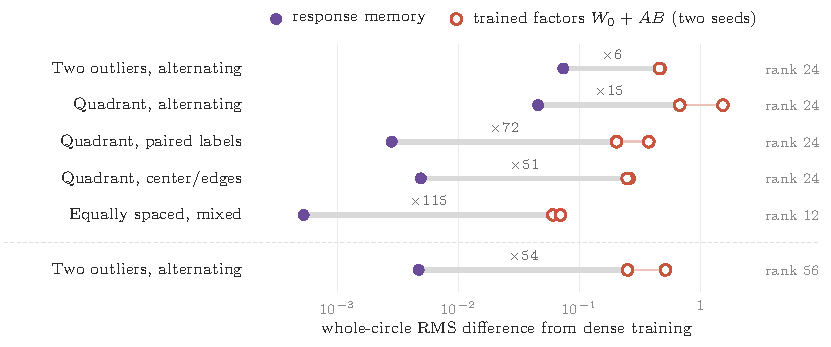
\includegraphics[width=0.9\textwidth]{figures/same_rank.pdf}
 \caption{\textbf{Same rank, different dynamics.} Whole-circle RMS difference
 from dense training for response memory and for a directly trained correction
 $W_0+AB$ of the middle matrix with the same rank (two factor seeds), two
 hidden tanh layers, width $2048$. Rank $24$ corresponds to $q=3$, rank $12$
 to $q=3$ on the four-representative antipodal quotient, and rank $56$ to $q=7$;
 labels give the smaller of the two ratios. Matched-loss endpoint comparisons
 against this specific factor baseline, not against every low-rank method;
 all ranks and the fitted functions are in \Cref{fig:factors}.}
 \label{fig:samerank-summary}
\end{figure}

\begin{figure}[!htbp]
 \centering
 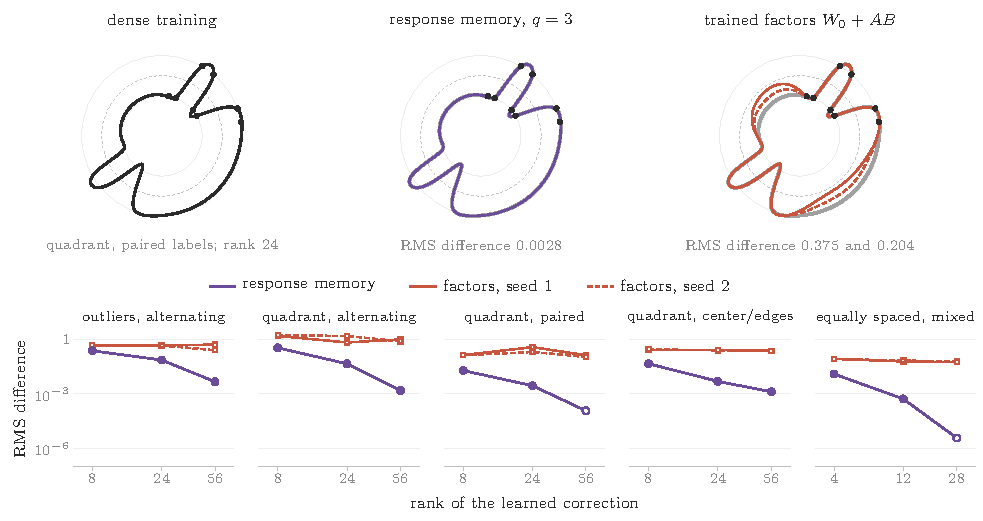
\includegraphics[width=\textwidth]{figures/factors.pdf}
 \caption{\textbf{Same correction rank, different fitted functions.} Two hidden
 tanh layers of width $2048$. Top: paired-label task, memory $q=3$ and both
 factor seeds at rank $24$, with the dense reference in black. Bottom: all
 five tasks at rank bounds $8,24,56$ (or $4,12,28$ for the exact antipodal
 quotient). Every model is shown at its own MSE $0.001$ endpoint; RMS uses
 $8192$ angles. Factors use $W_2=W_0+AB$, $A(0)=0$, independent
 $B_{ij}(0)\sim N(0,1/\mathrm{rank})$, and unit factor mobilities. Both outer
 layers have their canonical mobilities. Equal rank matches the factor-array
 budget, not total state or runtime. One capped comparison is omitted;
 hollow memory points have limited numerical precision.}
 \label{fig:factors}
\end{figure}

\clearpage
\begin{figure}[p]
 \centering
 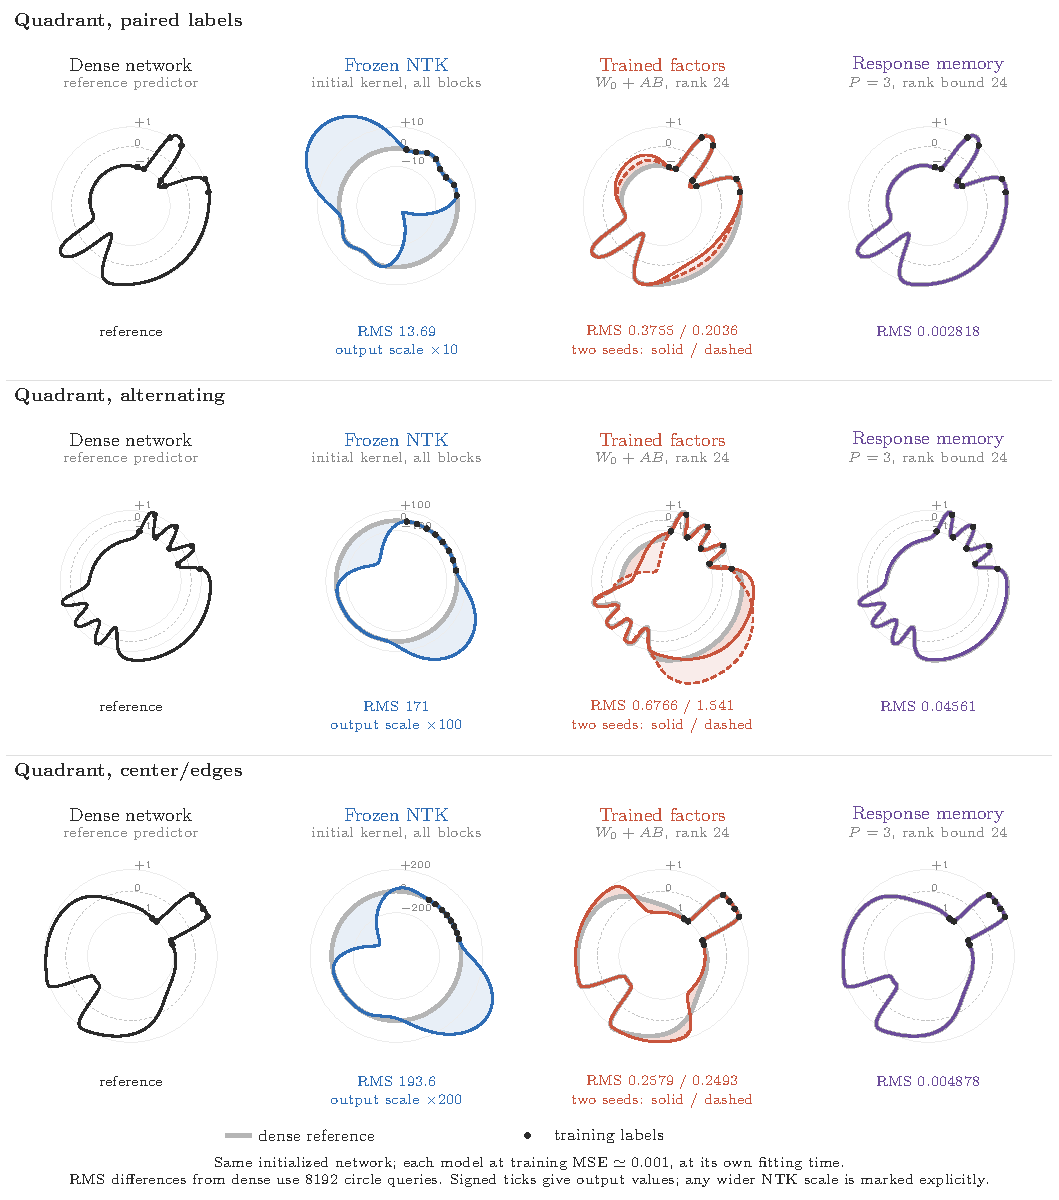
\includegraphics[width=\textwidth,height=0.78\textheight,keepaspectratio]{figures/learning_controls_gallery_a.pdf}
 \caption{\textbf{Four training descriptions on five circle tasks, part one.}
 Paired-label, alternating-label, and center/edges quadrant tasks. Columns
 show dense, frozen NTK, both directly trained factor seeds, and memory
 $q=3$. The latter two have correction rank bound $24$. Each model is at its
 own training-MSE $0.001$ endpoint. The NTK output scale is wider by the marked
 factor; signed ticks and RMS retain original output units. Gray is the dense
 reference, black dots are training labels, and RMS uses $8192$ circle queries.
 The next page continues with the remaining two tasks.}
 \label{fig:controls-gallery}
\end{figure}

\begin{figure}[p]
 \ContinuedFloat
 \centering
 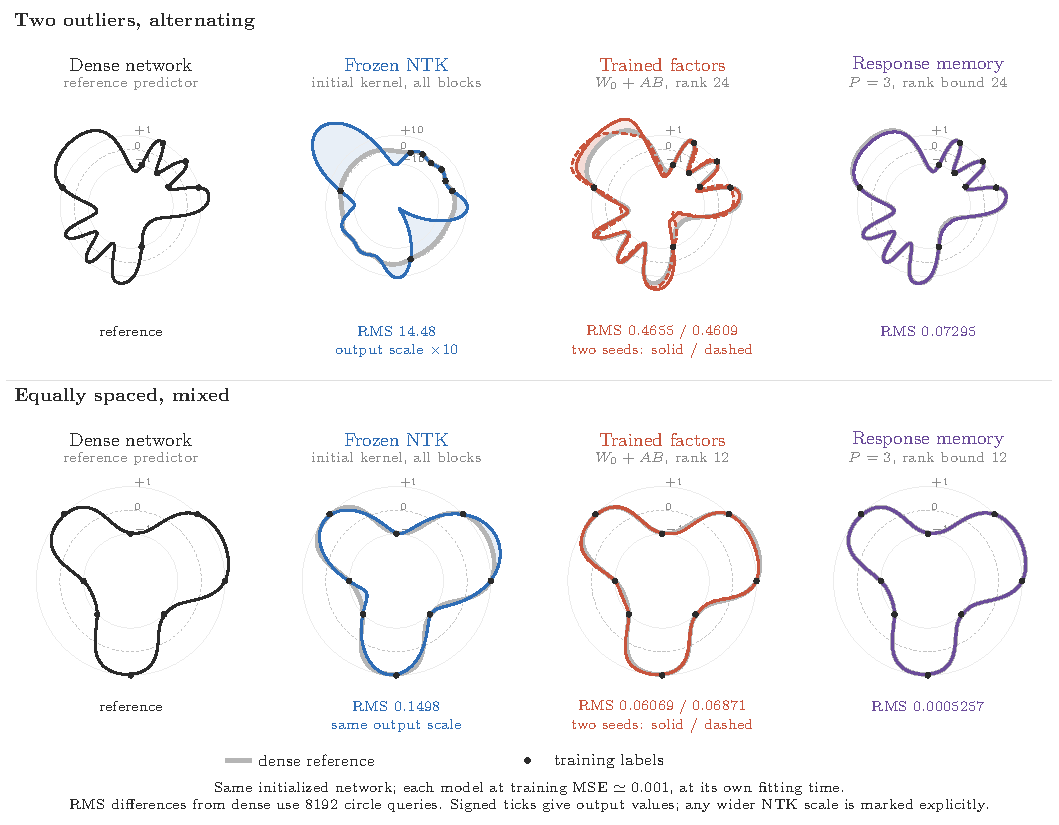
\includegraphics[width=\textwidth,height=0.78\textheight,keepaspectratio]{figures/learning_controls_gallery_b.pdf}
 \caption{\textbf{Four training descriptions on five circle tasks, continued.}
 Two-outlier alternating labels and equally spaced mixed labels. The latter
 uses four antipodal representatives and correction rank $12$; the former
 uses rank $24$. All eight physical training inputs are displayed. NTK uses
 a ten-times wider output scale for the outlier task and the same scale as
 the other methods for the equally spaced task. Models, endpoints, seeds,
 colors and RMS definitions follow the preceding page.}
\end{figure}

\end{document}
